\documentclass[a4paper]{scrartcl}

\usepackage[
fancytheorems,
fancyproofs,
noindent
]{adam}

\usepackage{tikz}
\usetikzlibrary{cd}
\usetikzlibrary{calc}
\usetikzlibrary{decorations.pathreplacing}

\newcommand{\charr}{\operatorname{char}}
\newcommand{\Gal}{\operatorname{Gal}}
\newcommand{\Tr}{\operatorname{Tr}}
\newcommand{\Nm}{\operatorname{N}}
\newcommand{\Frac}{\operatorname{Frac}}
\newcommand{\Disc}{\operatorname{Disc}}
\newcommand{\Frob}{\operatorname{Frob}}
\newcommand{\cbrt}[1]{\sqrt[3]{#1}}
\newcommand{\contra}{\raisebox{0.15ex}{\(\Rightarrow\!\Leftarrow\)}}

\title{Galois Theory}
\author{Adam Kelly (\texttt{ak2316@cam.ac.uk})}
\date{\today}

\allowdisplaybreaks

\begin{document}

\maketitle

Galois theory is the study of the symmetries of the solutions of polynomial equations. The central discovery of the subject -- and it really is one of the most beautiful discoveries in all of mathematics -- is that the messy analytic question `can I write down the roots of this polynomial using $+, -, \times, \div$ and $\sqrt[n]{\phantom{x}}$?' is exactly equivalent to a clean, finite, combinatorial question about a group. Galois' insight was to stop looking at the roots one at a time, and instead to look at the group of symmetries that permutes them without disturbing any of the algebra they satisfy.

Modern treatments phrase all of this in terms of \emph{field extensions}, and the heart of the course is a dictionary -- the \emph{Galois correspondence} -- translating between the subfields of a field extension and the subgroups of its symmetry group. Once we have that dictionary in hand, an enormous amount falls out: the impossibility of trisecting an angle, the classification of finite fields, the constructibility of the regular $17$-gon, the fundamental theorem of algebra, and of course the insolubility of the general quintic.

This article constitutes my notes for the `Galois Theory' course, held in Michaelmas 2021 at Cambridge. These notes are \emph{not a transcription of the lectures}, and differ significantly in quite a few areas. Still, all lectured material should be covered.

\tableofcontents

\section{Introduction}

\subsection{A Bit of History}

Historically the subject arose from looking at solutions to polynomial equations in one variable over $\C$. The question arose as to whether polynomials could be solved by a formula involving the coefficients and taking roots (`soluble by radicals'). From school, we know that we can solve quadratics in this way, with
$$x = \frac{-b \pm \sqrt{b^2 - 4ac}}{2a}.$$
For a long time it has been known that cubics and quartics have similar, albeit rather more complicated, formulae for their roots. These were studied by Lagrange in the 1770s, who was the first to notice that what really mattered was how certain expressions in the roots behaved when the roots were permuted.

In 1799 Ruffini claimed that there was no general formula in the case of quintics, however there was a gap in his proof. It wasn't until Abel in 1824 that there was a complete accepted proof, using permutations of roots of polynomials. This was the start of group theory.

Galois gave the first explanation of \emph{when} a quintic was soluble by radicals or not in 1831, using the structure of a group of permutations of the roots, and in particular the importance of normal subgroups. Galois' work was not known until Liouville published his papers in 1846. Liouville realised the connection with Cauchy's work on permutations, but didn't realise the importance of the group-theoretic structure, and in fact few of the contemporary mathematicians did so.

Galois entered his papers for various competitions and also for the entrance process for the \'Ecole Polytechnique in Paris. He didn't get in however, and went to another university in Paris, where he got involved in politics and was eventually killed in a duel at the age of twenty. The night before the duel he left a $6\frac{1}{2}$ page manuscript setting out his ideas about the future development of the theory. His papers have been carefully studied by Peter Neumann, in \emph{The Mathematical Writings of \'Evariste Galois} (History of European Mathematics, European Mathematical Society).

There is a historical introduction in I. Stewart's \emph{Galois Theory}, which is very readable but doesn't quite cover the syllabus. Other books worth looking at are Artin's \emph{Galois Theory}, Van der Waerden's \emph{Modern Algebra}, Lang's \emph{Algebra}, and Kaplansky's \emph{Fields and Rings}.

\subsection{Solving Cubics and Quartics}

Before we get going, it is worth reminding ourselves what these classical formulae actually look like, because the shape of the answer will turn out to be a very good guide to the shape of the theory.

Consider a cubic $f(x) = x^3 + ax^2 + bx + c$. Substituting $x \mapsto x - a/3$ (which is legitimate provided $\charr K \neq 3$) we may assume $a = 0$, so
$$f(x) = x^3 + px + q.$$
Cardano's trick is to write a root as $x = u + v$. Then
$$x^3 = u^3 + v^3 + 3uv(u+v) = u^3 + v^3 + 3uvx,$$
so $x$ is a root of $f$ provided that $u^3 + v^3 = -q$ and $3uv = -p$. But then $u^3$ and $v^3$ are two numbers with known sum $-q$ and known product $-p^3/27$, so they are the roots of a \emph{quadratic},
$$t^2 + qt - \frac{p^3}{27} = 0.$$
Solving that quadratic and taking cube roots gives the roots of $f$. What we should notice here is the intrusion of an auxiliary quadratic -- the \vocab{resolvent} -- and the fact that solving a cubic requires taking a square root and then a cube root, in that order. The quartic behaves similarly: an auxiliary \emph{cubic} appears, and the whole thing unravels into a chain of extractions of roots. The whole point of the course will be to explain \emph{why} such a chain must exist for degrees $2, 3, 4$, and why no such chain can exist for degree $5$.

\subsection{Notation and Revision}

Everything we do will take place inside rings and fields, and we will lean quite heavily on the Groups, Rings and Modules course. Let us fix our conventions and remind ourselves of what we need.

In this course a \vocab{ring} always means a commutative ring with a $1$, and ring homomorphisms are required to send $1 \mapsto 1$. A \vocab{field} is a ring in which every non-zero element is a unit, for instance $\Q, \R, \C$ and $\F_p = \Z/p\Z$ for $p$ prime. For a ring $R$ we write $R^\times$ for its group of units, so if $K$ is a field then $K^\times = K \setminus \{0\}$.

We write $R[x]$ for the ring of polynomials in an indeterminate $x$ with coefficients in $R$, that is, the set of formal sums $\sum_{i \geq 0} r_i x^i$ with all but finitely many $r_i$ equal to zero.\footnote{It is a good exercise to check that if $R$ is an integral domain then so is $R[x]$, and that in that case $\deg(fg) = \deg f + \deg g$.} If $K$ is a field, then $K(x)$ denotes the \vocab{field of fractions} of $K[x]$, whose elements are equivalence classes of formal quotients $f/g$ with $g \neq 0$, where $f/g = r/s$ exactly when $fs = gr$. Its elements are called \vocab{rational functions}.

The single most important fact we import from Groups, Rings and Modules is that polynomial rings over a field are as well-behaved as we could possibly hope.

\begin{theorem}[Division Algorithm]
	Let $K$ be a field and let $a, b \in K[x]$ with $b \neq 0$. Then there exist $q, r \in K[x]$ with
	$$a = qb + r, \qquad \deg r < \deg b.$$
	In other words, $K[x]$ is a Euclidean domain.
\end{theorem}

Everything else we need is a formal consequence.

\begin{corollary}
	Let $K$ be a field. Then:
	\begin{enumerate}[label=(\roman*)]
		\item $K[x]$ is a principal ideal domain;
		\item $K[x]$ is a unique factorisation domain;
		\item for $f \in K[x]$ non-constant, $f$ is irreducible $\iff$ $f$ is prime $\iff$ $(f)$ is maximal $\iff$ $K[x]/(f)$ is a field;
		\item for $a, b \in K[x]$, the ideal $(a) + (b)$ equals $(g)$ for some $g$, and this $g$ is a greatest common divisor of $a$ and $b$, unique up to a unit. In particular $\gcd(a,b) = pa + qb$ for some $p, q \in K[x]$;
		\item if $f \in K[x] \setminus \{0\}$ then $f$ has at most $\deg f$ roots in $K$.\footnote{As usual, $\alpha$ is a \vocab{root} of $f$ if $f(\alpha) = 0$, and by the division algorithm this happens if and only if $(x - \alpha) \mid f$.}
	\end{enumerate}
\end{corollary}

\begin{proof}
	All of these were proved in Groups, Rings and Modules; (i) follows by taking a non-zero element of least degree in an ideal and dividing, (ii) follows since every PID is a UFD, (iii) is the standard characterisation of irreducibles in a PID, (iv) is immediate from (i), and (v) follows from (ii) together with the factor theorem.
\end{proof}

The point of (iii) that we will use again and again is the following: \emph{if $f \in K[x]$ is irreducible, then $K[x]/(f)$ is a field}. This is the engine that manufactures new fields out of old ones, and it is where the whole subject starts.

We will also want the standard irreducibility criteria from Groups, Rings and Modules, namely Gauss's lemma (a primitive polynomial in $\Z[x]$ is irreducible in $\Z[x]$ if and only if it is irreducible in $\Q[x]$) and Eisenstein's criterion.

\section{Field Extensions}

\subsection{Extensions and Degree}

The basic object of the course is not a field but a \emph{pair} of fields, one sitting inside the other.

\begin{definition}[Field Extension]
	If $K \subseteq L$ where $L$ is a field and $K$ is a subring of $L$ which is itself a field, then we say $L$ is an \vocab{extension} of $K$, and write $L/K$.\footnote{The notation $L/K$ has nothing whatsoever to do with quotients. It is unfortunate, but universal.}
\end{definition}

For example $\C/\R$, $\R/\Q$ and $K(x)/K$ are all field extensions, as is $L/K$ where $L = K[x]/(f)$ for $f \in K[x]$ irreducible (here we regard $K$ as sitting inside $L$ as the constant polynomials).

Now here is the observation that makes the whole theory work. If $L/K$ is a field extension, then $L$ is in particular a vector space over $K$: we can add elements of $L$, and we can multiply them by scalars from $K$, and all of the vector space axioms are instances of the field axioms in $L$. So we may bring the whole of linear algebra to bear.

\begin{definition}[Degree]
	The \vocab{degree} of a field extension $L/K$ is
	$$[L : K] = \dim_K L,$$
	the dimension of $L$ as a $K$-vector space. If $[L:K] < \infty$ we say $L/K$ is a \vocab{finite} extension, and otherwise an \vocab{infinite} extension.
\end{definition}

For instance $[\C : \R] = 2$, since $\{1, i\}$ is an $\R$-basis of $\C$. On the other hand $[\R : \Q] = \infty$, and $[K(x) : K] = \infty$ since $1, x, x^2, \dots$ are linearly independent over $K$.

Before going further, let us record the smallest subfield that any field contains.

\begin{definition}[Characteristic]
	Let $K$ be a field. There is a unique ring homomorphism $\Z \to K$, sending $1 \mapsto 1$. If it is injective then $K$ contains a copy of $\Q$ and we say $K$ has \vocab{characteristic} zero, written $\charr K = 0$. Otherwise its kernel is a non-zero prime ideal $(p)$, so that $\underbrace{1 + 1 + \dots + 1}_{p} = 0$ in $K$; then $K$ contains a copy of $\F_p$ and we say $\charr K = p$.
\end{definition}

The kernel must be prime because its quotient embeds in the integral domain $K$. In either case the image of $\Z \to K$ generates a smallest subfield of $K$, called the \vocab{prime subfield}, which is $\Q$ or $\F_p$ accordingly. For instance $\charr \F_p(x) = p$, since $p \cdot 1 = 0$ already in $\F_p$.

We say $K$ is a \vocab{finite field} if $\#K < \infty$, where $\#K$ denotes the number of elements of $K$. Already we can say something about what sizes are possible.

\begin{lemma}
	If $F$ is a finite field then $\charr F = p$ for some prime $p$, and $\#F = p^n$ where $n = [F : \F_p]$.
\end{lemma}

\begin{proof}
	If $\#F < \infty$ then the map $\Z \to F$ cannot be injective, so $\charr F = p$ for some prime $p$ and $\F_p \subseteq F$. Then $F$ is a vector space over $\F_p$, necessarily finite-dimensional, say of dimension $n$. Choosing a basis gives an isomorphism of $\F_p$-vector spaces $F \cong \F_p^n$, and hence $\#F = p^n$.
\end{proof}

We will see later that, conversely, for every prime $p$ and every $n \geq 1$ there is a field with $p^n$ elements, and that it is unique up to isomorphism.

\subsection{The Tower Law}

Degrees behave exactly as you would want them to in a tower of extensions -- they multiply. This little fact is used constantly, often several times on the same page.

\begin{theorem}[Tower Law]
	Let $M/L/K$ be field extensions. Then $M/K$ is finite if and only if both $M/L$ and $L/K$ are finite, and in that case
	$$[M : K] = [M : L][L : K].$$
\end{theorem}

It is no harder, and rather more useful, to prove the following slightly more general statement about vector spaces.

\begin{proposition}\label{prop:towervs}
	Let $L/K$ be a finite field extension and let $V$ be a vector space over $L$. Then $V$ is finite dimensional over $L$ if and only if it is finite dimensional over $K$, and in that case
	$$\dim_K V = \dim_L V \cdot [L : K].$$
\end{proposition}

\begin{proof}
	Suppose $\dim_L V = d < \infty$, and take an $L$-basis $\alpha_1, \dots, \alpha_d$ of $V$ and a $K$-basis $\ell_1, \dots, \ell_n$ of $L$. We claim that the $nd$ products
	$$\{\ell_i \alpha_j : 1 \leq i \leq n,\ 1 \leq j \leq d\}$$
	form a $K$-basis of $V$.

	They span: any $v \in V$ can be written $v = \sum_{j} \mu_j \alpha_j$ with $\mu_j \in L$, and each $\mu_j = \sum_i \lambda_{ij} \ell_i$ with $\lambda_{ij} \in K$, so $v = \sum_{i,j} \lambda_{ij} \ell_i \alpha_j$.

	They are independent: if $\sum_{i,j} \lambda_{ij} \ell_i \alpha_j = 0$ with $\lambda_{ij} \in K$, then collecting terms gives $\sum_j \left( \sum_i \lambda_{ij}\ell_i \right)\alpha_j = 0$, and the inner brackets lie in $L$, so by $L$-independence of the $\alpha_j$ each $\sum_i \lambda_{ij} \ell_i = 0$, and then by $K$-independence of the $\ell_i$ each $\lambda_{ij} = 0$.

	Hence $\dim_K V = nd = \dim_L V \cdot [L:K] < \infty$.

	Conversely if $\dim_K V < \infty$ then certainly $\dim_L V < \infty$, since a $K$-spanning set is in particular an $L$-spanning set.
\end{proof}

\begin{proof}[Proof of the Tower Law]
	If $L/K$ is infinite then $L \subseteq M$ forces $M/K$ to be infinite, and if $M/L$ is infinite then so is $M/K$ by the same argument applied to a set of elements of $M$ independent over $L$. Otherwise apply Proposition \ref{prop:towervs} with $V = M$.
\end{proof}

It is worth pausing to appreciate how much arithmetic information the tower law encodes. If we can find a subfield of $L$ containing $K$, its degree over $K$ must divide $[L:K]$; contrapositively, if $[L:K]$ is prime then there are no intermediate fields at all. This kind of numerical reasoning is remarkably powerful, and we will use it immediately.

\subsection{Algebraic and Transcendental Elements}

Given a field extension $L/K$ and an element $\alpha \in L$, we write $K[\alpha]$ for the smallest subring of $L$ containing both $K$ and $\alpha$, and $K(\alpha)$ for the smallest subfield. Concretely,
$$K[\alpha] = \left\{ \sum_{i=0}^N r_i \alpha^i : r_i \in K, N \in \N \right\}, \qquad K(\alpha) = \left\{ f/g : f, g \in K[\alpha], g \neq 0 \right\}.$$
More generally we write $K(\alpha_1, \dots, \alpha_n)$ for the smallest subfield of $L$ containing $K$ and all the $\alpha_i$; note that $K(\alpha, \beta) = (K(\alpha))(\beta)$, so we can adjoin elements one at a time.

\begin{example}
	Take $L = \C$, $K = \Q$ and $\alpha = i$. Then
	$$\Q[i] = \{a_0 + a_1 i + a_2 i^2 + \dots + a_n i^n : a_j \in \Q\} = \{a + bi : a, b \in \Q\},$$
	since $i^2 = -1$ lets us collapse all the higher powers. This is already a field, because $(a+bi)^{-1} = (a - bi)/(a^2+b^2)$, and so $\Q(i) = \Q[i]$.
\end{example}

That last coincidence -- that $K[\alpha]$ happened to be a field already -- is not an accident, and understanding exactly when it happens is the content of this subsection. The right way to see it is through the evaluation map.

Fix $\alpha \in L$ and consider the ring homomorphism
$$\phi : K[x] \to L, \qquad x \mapsto \alpha,$$
which is to say $\phi\left(\sum r_i x^i\right) = \sum r_i \alpha^i$. Its image is exactly $K[\alpha]$. There are then precisely two possibilities, according to whether $\phi$ is injective.

\begin{definition}[Algebraic and Transcendental]
	With notation as above, we say $\alpha$ is \vocab{transcendental} over $K$ if $\phi$ is injective, and \vocab{algebraic} over $K$ if $\phi$ is not injective. Equivalently, $\alpha$ is algebraic over $K$ if and only if $f(\alpha) = 0$ for some non-zero $f \in K[x]$.
\end{definition}

Suppose $\alpha$ is algebraic. Then $\ker \phi$ is a non-zero ideal of the PID $K[x]$, so $\ker \phi = (f)$ for some non-zero $f$, unique up to a unit; normalising so that $f$ is monic pins it down completely.

\begin{definition}[Minimal Polynomial]
	Let $\alpha \in L$ be algebraic over $K$. The \vocab{minimal polynomial} of $\alpha$ over $K$ is the unique monic generator $f$ of $\ker(\phi : K[x] \to L)$. Equivalently, it is the monic polynomial of least degree in $K[x]$ having $\alpha$ as a root, and it divides every polynomial in $K[x]$ with $\alpha$ as a root. We write $\deg_K \alpha = \deg f$ for the \vocab{degree} of $\alpha$ over $K$.
\end{definition}

\begin{lemma}
	The minimal polynomial of $\alpha$ over $K$ is irreducible in $K[x]$.
\end{lemma}

\begin{proof}
	Write $f$ for the minimal polynomial, and suppose $f = gh$ with $\deg g, \deg h < \deg f$. Then $g(\alpha)h(\alpha) = f(\alpha) = 0$ in $L$, and $L$ is a field and hence an integral domain, so $g(\alpha) = 0$ or $h(\alpha) = 0$. Either way we have found a non-zero polynomial of smaller degree than $f$ vanishing at $\alpha$, contradicting minimality.
\end{proof}

Notice a small but useful consequence: since $f$ is irreducible and $\deg f \geq 1$, its constant term $a_0$ is non-zero (else $x \mid f$). Writing $f(x) = x^n + a_{n-1}x^{n-1} + \dots + a_0$ and rearranging $f(\alpha) = 0$ gives
$$\alpha \cdot \left( -\frac{1}{a_0}\left(\alpha^{n-1} + a_{n-1}\alpha^{n-2} + \dots + a_1 \right)\right) = 1,$$
so $\alpha^{-1} \in K[\alpha]$. This is the first hint that $K[\alpha]$ is a field whenever $\alpha$ is algebraic; here is the full statement.

\begin{proposition}\label{prop:algebraictfae}
	Let $L/K$ be a field extension and $\alpha \in L$. The following are equivalent:
	\begin{enumerate}[label=(\roman*)]
		\item $\alpha$ is algebraic over $K$;
		\item $[K(\alpha) : K] < \infty$;
		\item $\dim_K K[\alpha] < \infty$;
		\item $K[\alpha] = K(\alpha)$;
		\item $K[\alpha]$ is a field.
	\end{enumerate}
	When these hold, $[K(\alpha) : K] = \deg_K \alpha$, and $1, \alpha, \dots, \alpha^{d-1}$ is a $K$-basis of $K(\alpha)$, where $d = \deg_K \alpha$.
\end{proposition}

\begin{proof}
	Suppose (i), and let $f$ be the minimal polynomial of $\alpha$, of degree $d$. Since $\phi$ has kernel $(f)$, the first isomorphism theorem gives $K[\alpha] \cong K[x]/(f)$, which is a field because $f$ is irreducible; this is (v), and (iv) follows since $K(\alpha)$ is the smallest field containing $K$ and $\alpha$. Moreover $1, \alpha, \dots, \alpha^{d-1}$ span $K[\alpha]$ (divide by $f$ and take the remainder) and are linearly independent (a linear relation would be a polynomial of degree $< d$ killing $\alpha$), so $\dim_K K[\alpha] = d$, giving (iii) and (ii).

	Conversely suppose (iii), so $\dim_K K[\alpha] = m < \infty$. Then $1, \alpha, \dots, \alpha^m$ are $m+1$ elements of an $m$-dimensional space, hence linearly dependent over $K$, and a non-trivial dependence is precisely a non-zero polynomial vanishing at $\alpha$. So (iii) $\Rightarrow$ (i). Since (ii) $\Rightarrow$ (iii) (as $K[\alpha] \subseteq K(\alpha)$) and (v) $\Rightarrow$ (iv) $\Rightarrow$ (i) (if $K[\alpha]$ is a field then $\alpha^{-1} \in K[\alpha]$, so $\alpha^{-1} = \sum r_i \alpha^i$ and hence $\alpha$ satisfies $\sum r_i x^{i+1} - 1 = 0$), all five are equivalent.
\end{proof}

The transcendental case is much less interesting, precisely because there is only one of them.

\begin{proposition}
	$\alpha$ is transcendental over $K$ if and only if $\phi : K[x] \to K[\alpha]$ is an isomorphism, in which case it extends to an isomorphism $K(x) \to K(\alpha)$. In particular, any two simple transcendental extensions of $K$ are $K$-isomorphic, both being isomorphic to the rational function field $K(x)$.
\end{proposition}

\begin{proof}
	The map $\phi$ is surjective onto $K[\alpha]$ by definition, so it is an isomorphism precisely when it is injective, which is the definition of transcendence. An isomorphism of integral domains extends uniquely to their fields of fractions, giving $K(x) \cong K(\alpha)$.
\end{proof}

\begin{remark}
	Both `algebraic' and `transcendental', and the minimal polynomial itself, depend very much on the base field $K$, and it is worth being careful about this.
	\begin{enumerate}[label=(\roman*)]
		\item $2\pi i \in \C$ is algebraic over $\R$, with minimal polynomial $x^2 + 4\pi^2$, but it is transcendental over $\Q$ (this is Lindemann's theorem, and is decidedly not easy).
		\item Let $\alpha = \sqrt{i} = \tfrac{\sqrt 2}{2}(1 + i)$. Over $\Q$ the minimal polynomial of $\alpha$ is $x^4 + 1$, whereas over $\Q(i)$ it is $x^2 - i$. Note that
		$$[\Q(i):\Q] = 2, \quad [\Q(\alpha):\Q(i)] = 2, \quad [\Q(\alpha):\Q] = 4,$$
		which is a first illustration of the tower law in action.
	\end{enumerate}
\end{remark}

\subsection{Working with Degrees}

Combining the tower law with Proposition \ref{prop:algebraictfae} gives a very effective toolkit. Here is the basic divisibility statement.

\begin{corollary}\label{cor:degdivides}
	If $L/K$ is a finite extension and $\alpha \in L$, then $\alpha$ is algebraic over $K$ and $\deg_K \alpha \mid [L:K]$.
\end{corollary}

\begin{proof}
	Since $K \subseteq K(\alpha) \subseteq L$ and $[L:K] < \infty$, we get $[K(\alpha):K] < \infty$, so $\alpha$ is algebraic. The tower law applied to $L/K(\alpha)/K$ gives $[L:K] = [L:K(\alpha)] \cdot \deg_K \alpha$.
\end{proof}

The following picture is the one to keep in mind: an element $\alpha \in L$ interposes an intermediate field, and the two degrees multiply to give the degree of the whole tower.

\begin{center}
	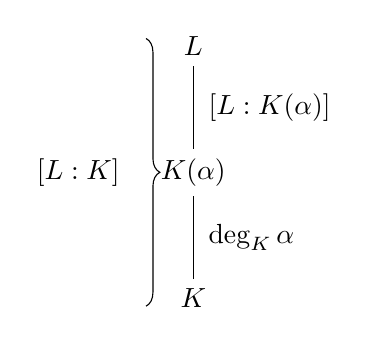
\begin{tikzpicture}[scale=1]
		\node (K) at (0,0) {$K$};
		\node (Ka) at (0,1.6) {$K(\alpha)$};
		\node (L) at (0,3.2) {$L$};
		\draw (K) -- node[right=2pt] {$\deg_K \alpha$} (Ka);
		\draw (Ka) -- node[right=2pt] {$[L : K(\alpha)]$} (L);
		\draw[decorate, decoration={brace, amplitude=5pt, mirror}] (-0.6,-0.1) -- node[left=6pt] {$[L:K]$} (-0.6,3.3);
	\end{tikzpicture}
\end{center}

\begin{example}
	Let us see the toolkit at work.
	\begin{enumerate}[label=(\roman*)]
		\item Suppose $[L:K] = p$ is prime. Then for every $\alpha \in L \setminus K$ we have $L = K(\alpha)$. Indeed $[K(\alpha):K]$ divides $p$, so is $1$ or $p$; it is not $1$ since $\alpha \notin K$; so $[K(\alpha):K] = p$ and hence $[L:K(\alpha)] = 1$.
		\item Every irreducible polynomial $f \in \R[x]$ has degree $1$ or $2$. Granting that $\C$ is algebraically closed, $f$ has a root $\alpha \in \C$, and $\deg f = [\R(\alpha):\R]$ divides $[\C:\R] = 2$.
		\item Let $L = \Q(\sqrt[3]{2}, \sqrt[4]{5})$. We claim $[L:\Q] = 12$. Certainly $L \supseteq \Q(\sqrt[3]2)$, and $x^3 - 2$ is irreducible over $\Q$ by Eisenstein at $2$, so $[\Q(\sqrt[3]2):\Q] = 3$ and hence $3 \mid [L:\Q]$. Similarly $x^4 - 5$ is irreducible by Eisenstein at $5$, so $4 \mid [L:\Q]$, and therefore $12 \mid [L:\Q]$. On the other hand $\sqrt[4]{5}$ satisfies $x^4 - 5$ over $\Q(\sqrt[3]2)$, so $[L : \Q(\sqrt[3]{2})] \leq 4$ and hence $[L:\Q] \leq 12$. So $[L:\Q] = 12$.
		\item Let $p$ be an odd prime, let $\omega = e^{2\pi i/p}$ and let $\alpha = \omega + \omega^{-1} = 2\cos(2\pi/p)$. What is $\deg_\Q \alpha$? Now $\omega$ is a root of
		$$f(x) = 1 + x + \dots + x^{p-1} = \frac{x^p - 1}{x - 1},$$
		which is irreducible over $\Q$: applying Eisenstein at $p$ to $f(x+1)$ does the job, since $f(x+1) = \frac{(x+1)^p - 1}{x} = x^{p-1} + \binom{p}{1}x^{p-2} + \dots + \binom{p}{p-1}$. Hence $[\Q(\omega):\Q] = p - 1$. Clearly $\alpha \in \Q(\omega)$, so $\Q(\omega)/\Q(\alpha)/\Q$ is a tower and $\deg_\Q \alpha \mid p-1$. Now $\alpha \omega = \omega^2 + 1$, so $\omega$ is a root of $x^2 - \alpha x + 1 \in \Q(\alpha)[x]$, giving $[\Q(\omega):\Q(\alpha)] \leq 2$. It is not $1$, since $\alpha \in \R$ but $\omega \notin \R$, so $[\Q(\omega):\Q(\alpha)] = 2$ and hence
		$$\deg_\Q \alpha = \frac{p-1}{2}.$$
	\end{enumerate}
\end{example}

Next, a fact that ought to be surprising: the algebraic elements are closed under all the field operations, even though there is no obvious way to write down the minimal polynomial of a sum.

\begin{corollary}\label{cor:algclosed}
	Let $L/K$ be a field extension.
	\begin{enumerate}[label=(\roman*)]
		\item Elements $\alpha_1, \dots, \alpha_n \in L$ are all algebraic over $K$ if and only if $[K(\alpha_1, \dots, \alpha_n) : K] < \infty$.
		\item If $\alpha, \beta \in L$ are algebraic over $K$ then so are $\alpha \pm \beta$, $\alpha\beta$ and $\alpha/\beta$ (the last provided $\beta \neq 0$).
	\end{enumerate}
\end{corollary}

\begin{proof}
	For (i), suppose first that $[K(\alpha_1, \dots, \alpha_n):K] < \infty$. Each $\alpha_i$ lies in this finite extension, so is algebraic over $K$ by Corollary \ref{cor:degdivides}. Conversely, suppose each $\alpha_i$ is algebraic over $K$. Then $\alpha_n$ is in particular algebraic over the larger field $K(\alpha_1, \dots, \alpha_{n-1})$ (its minimal polynomial over $K$ is still a polynomial there), so
	$$[K(\alpha_1, \dots, \alpha_n) : K(\alpha_1, \dots, \alpha_{n-1})] < \infty,$$
	and the result follows by induction and the tower law, as a product of finitely many finite numbers.

	For (ii), all four elements lie in $K(\alpha, \beta)$, which is a finite extension of $K$ by (i), so all four are algebraic by Corollary \ref{cor:degdivides}.
\end{proof}

\begin{corollary}
	The elements of $L$ which are algebraic over $K$ form a subfield of $L$.
\end{corollary}

It is instructive to see how one might find an explicit polynomial in a simple case -- this is the sort of thing that Galois theory will eventually let us do systematically.

\begin{example}
	Let $a, b \in K$ and let $\alpha = \sqrt a$, $\beta = \sqrt b$ in some extension. Put $\gamma = \alpha + \beta$. We compute, using $\alpha^2 = a$ and $\beta^2 = b$:
	\begin{align*}
		\gamma^2 &= a + b + 2\alpha\beta, \\
		\gamma^4 &= (a+b)^2 + 4\alpha\beta(a+b) + 4ab,
	\end{align*}
	and $2(a+b)\gamma^2 = 2(a+b)^2 + 4\alpha\beta(a+b)$. Subtracting kills the awkward $\alpha\beta$ term:
	$$\gamma^4 - 2(a+b)\gamma^2 = 4ab - (a+b)^2 = -(a-b)^2.$$
	So $\gamma$ is a root of $x^4 - 2(a+b)x^2 + (a-b)^2$.
\end{example}

More generally, if $\deg_K \alpha = m$ and $\deg_{K(\alpha)} \beta = n$, then $K(\alpha,\beta)$ is spanned over $K$ by the $mn$ monomials $\alpha^i \beta^j$ with $0 \leq i < m$, $0 \leq j < n$. So for any $\gamma \in K(\alpha,\beta)$, the $mn+1$ elements $1, \gamma, \dots, \gamma^{mn}$ must be linearly dependent over $K$, which produces a polynomial of degree at most $mn$ satisfied by $\gamma$. Be warned that the polynomial obtained this way is in general \emph{not} the minimal polynomial.

\begin{exercise}
	Show that if $m, n, mn \in \Q$ are all non-squares, then $[\Q(\sqrt m + \sqrt n):\Q] = 4$.
\end{exercise}

\subsection{Algebraic Extensions}

\begin{definition}[Algebraic Extension]
	An extension $L/K$ is an \vocab{algebraic extension} if every $\alpha \in L$ is algebraic over $K$.
\end{definition}

By Corollary \ref{cor:degdivides}, every finite extension is algebraic. The converse fails.

\begin{example}
	Let $\overline{\Q} = \{\alpha \in \C : \alpha \text{ is algebraic over } \Q\}$, the field of \vocab{algebraic numbers} (a field, by Corollary \ref{cor:algclosed}). Then $\overline{\Q}/\Q$ is algebraic by construction, but it is not finite: $\sqrt[n]{2} \in \overline\Q$ has degree $n$ over $\Q$ for every $n$, so $[\overline\Q : \Q] \geq n$ for all $n$.
\end{example}

\begin{proposition}\label{prop:algebraictower}
	\begin{enumerate}[label=(\roman*)]
		\item Every finite extension is algebraic.
		\item If $M/L/K$ are field extensions, then $M/K$ is algebraic if and only if $M/L$ and $L/K$ are algebraic.
	\end{enumerate}
\end{proposition}

\begin{proof}
	Part (i) is Corollary \ref{cor:degdivides}.

	For (ii), suppose first $M/K$ is algebraic. If $\alpha \in M$ then $\alpha$ is algebraic over $K$, hence over the larger field $L$; and $L \subseteq M$, so every element of $L$ is algebraic over $K$ too.

	Conversely suppose $M/L$ and $L/K$ are algebraic, and let $\alpha \in M$. Then $\alpha$ is algebraic over $L$, so
	$$r_0 + r_1\alpha + \dots + r_d\alpha^d = 0$$
	for some $r_0, \dots, r_d \in L$ not all zero. Put $L_0 = K(r_0, \dots, r_d)$. Each $r_j$ is algebraic over $K$ since $L/K$ is algebraic, so $[L_0 : K] < \infty$ by Corollary \ref{cor:algclosed}. Also $\alpha$ is algebraic over $L_0$ by the displayed equation, so $[L_0(\alpha):L_0] < \infty$. By the tower law
	$$[L_0(\alpha) : K] = [L_0(\alpha):L_0][L_0:K] < \infty,$$
	and $\alpha$ lies in this finite extension of $K$, hence is algebraic over $K$.
\end{proof}

In other words, an extension $L/K$ is algebraic exactly when $L$ is a union of subfields each of which is finite over $K$.

\section{Ruler and Compass Constructions}\label{sec:construct}

This section is an interlude, but a very satisfying one. The Greeks asked a number of geometric questions which resisted attack for two thousand years: can we trisect a general angle with ruler and compass? Can we construct a square with the same area as a given circle? Can we construct a cube with double the volume of a given cube? With the tower law in hand, all three become easy.

\subsection{What Is Constructible?}

We begin with two marked points in the plane, which we declare to be \vocab{constructed}. From a set of constructed points we may produce more, as follows: given constructed points we may draw the line through any two of them, and the circle centred at one of them passing through another, and then any point of intersection of two such lines, of two such circles, or of a line and a circle, is again constructed. A point is \vocab{constructible} if it can be obtained from the two initial points by finitely many such steps.

\begin{center}
	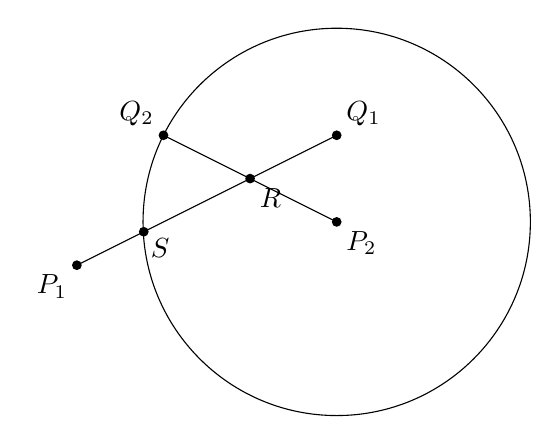
\begin{tikzpicture}[scale=1.1]
		\draw[thin] (2.5,0.3) circle (2.236);
		\draw[thin] (-0.5,-0.2) -- (2.5,1.3);
		\draw[thin] (2.5,0.3) -- (0.5,1.3);
		\fill (-0.5,-0.2) circle (1.6pt) node[below left] {$P_1$};
		\fill (2.5,0.3) circle (1.6pt) node[below right] {$P_2$};
		\fill (0.5,1.3) circle (1.6pt) node[above left] {$Q_2$};
		\fill (2.5,1.3) circle (1.6pt) node[above right] {$Q_1$};
		\fill (1.5,0.8) circle (1.6pt) node[below right] {$R$};
		\fill (0.2725,0.1863) circle (1.6pt) node[below right=-1pt] {$S$};
	\end{tikzpicture}
\end{center}

In the picture, $R$ is the intersection of the lines $P_1Q_1$ and $P_2Q_2$, and $S$ is one of the two intersections of the line $P_1Q_1$ with the circle centred at $P_2$ passing through $Q_2$; both are therefore constructible from $P_1, P_2, Q_1, Q_2$.

There are three standard constructions that we shall use freely, all of which are done in school.

\begin{enumerate}[label=(\roman*)]
	\item Given a constructed point $P$ and a constructed line $\ell$, we may drop or erect the perpendicular to $\ell$ through $P$. (Draw a circle centred at $P$ meeting $\ell$ in two points $A, B$; then circles of equal radius centred at $A$ and $B$ meet in two points, and the line through those two points is the required perpendicular.)
	\item Given a constructed point $P$ and a constructed line $\ell$, we may draw the line through $P$ parallel to $\ell$: erect the perpendicular $m$ to $\ell$ through $P$, then the perpendicular to $m$ through $P$.
	\item Given constructed points $a, b$ and a constructed point $P$ on a constructed line $\ell$, we may mark off the length $|ab|$ along $\ell$ starting from $P$: this is what a compass is for.
\end{enumerate}

As a consequence of (i) and (ii) we may set up Cartesian coordinates, declaring our two initial points to be $(0,0)$ and $(1,0)$, and constructing the two coordinate axes.

\begin{definition}[Constructible Number]
	A real number $\lambda$ is \vocab{constructible} if $|\lambda|$ is the distance between two constructible points.
\end{definition}

\begin{lemma}
	A point $P = (a,b)$ is constructible if and only if $a$ and $b$ are constructible real numbers.
\end{lemma}

\begin{proof}
	If $P$ is constructible, drop perpendiculars from $P$ onto the two axes; the feet are constructible points, at distances $|a|$ and $|b|$ from the origin. Conversely, given constructible $a$ and $b$, mark off $a$ along the $x$-axis and $b$ along the $y$-axis, erect perpendiculars there, and take their intersection.
\end{proof}

\subsection{Constructible Numbers Form a Field}

\begin{proposition}
	The set of constructible real numbers is a subfield of $\R$, closed moreover under taking square roots of positive elements.
\end{proposition}

\begin{proof}
	Let $a, b$ be constructible. Then $a + b$ and $-a$ are constructible by marking off lengths along a line, so we have an additive subgroup containing $\Q$.

	For products and quotients we use similar triangles. Draw two rays from a point $O$. Along the first mark points $U$ and $A$ at distances $1$ and $a$; along the second mark $B$ at distance $b$. Draw the line $UB$, and then the line through $A$ parallel to it, meeting the second ray at $C$. By similarity $|OC|/|OB| = |OA|/|OU|$, that is $|OC| = ab$.

	\begin{center}
		\begin{tikzpicture}[scale=1.05]
			\coordinate (O) at (0,0);
			\coordinate (U) at (1.1,0);
			\coordinate (A) at (3.3,0);
			\coordinate (B) at (0.85,1.36);
			\coordinate (C) at (2.55,4.08);
			\draw[thin] (O) -- (4.1,0);
			\draw[thin] (O) -- node[pos=0.5, above left=-2pt] {$b$} (B)
			              -- node[pos=0.5, above left=-2pt] {$ab$} (C) -- (2.9,4.64);
			\draw[thin] (U) -- (B);
			\draw[thin] (A) -- (C);
			\fill (O) circle (1.5pt) node[below left] {$O$};
			\fill (U) circle (1.5pt) node[below] {$U$};
			\fill (A) circle (1.5pt) node[below] {$A$};
			\fill (B) circle (1.5pt) node[right=2pt] {$B$};
			\fill (C) circle (1.5pt) node[right=2pt] {$C$};
			\node at (0.55,0.18) {$1$};
			\draw[decorate, decoration={brace, amplitude=4pt, mirror}] (0,-0.45) -- node[below=4pt] {$a$} (3.3,-0.45);
		\end{tikzpicture}
	\end{center}

	Exactly the same picture read backwards gives $a/b$ for $b \neq 0$: mark $b$ and $1$ on the first ray and $a$ on the second.

	Finally, suppose $a > 0$ is constructible. Mark off a segment of length $a$ followed by a segment of length $1$ along a line, giving a segment $XZ$ of length $a+1$ with the intermediate point $Y$. Draw the semicircle on $XZ$ as diameter, and erect the perpendicular to $XZ$ at $Y$, meeting the semicircle at $W$. The angle $XWZ$ is a right angle (angle in a semicircle), so the triangles $XYW$ and $WYZ$ are similar, giving $|YW|^2 = |XY||YZ| = a$, so $|YW| = \sqrt a$.

	\begin{center}
		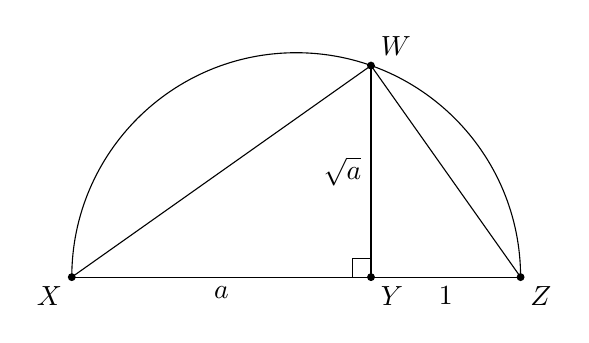
\begin{tikzpicture}[scale=0.95]
			\draw[thin] (0,0) -- node[below] {$a$} (4,0);
			\draw[thin] (4,0) -- node[below] {$1$} (6,0);
			\draw[thin] (3,0) ++(0:3) arc (0:180:3);
			\draw[thin] (4,0) -- node[left] {$\sqrt a$} (4,2.828);
			\draw[thin] (0,0) -- (4,2.828) -- (6,0);
			\draw (4,0) rectangle (3.75,0.25);
			\fill (0,0) circle (1.5pt) node[below left] {$X$};
			\fill (4,0) circle (1.5pt) node[below right] {$Y$};
			\fill (6,0) circle (1.5pt) node[below right] {$Z$};
			\fill (4,2.828) circle (1.5pt) node[above right] {$W$};
		\end{tikzpicture}
	\end{center}
	\vspace{-1em}
\end{proof}

That is the easy half. The point of the theory is the other half: nothing else is constructible.

\begin{theorem}\label{thm:construct}
	A real number $\lambda$ is constructible if and only if there is a chain of subfields
	$$\Q = F_0 \subseteq F_1 \subseteq \dots \subseteq F_n = F \subseteq \R$$
	with $\lambda \in F$, where for each $j$ we have $F_{j+1} = F_j(\sqrt{r_j})$ for some $r_j \in F_j$ with $r_j > 0$.
\end{theorem}

\begin{proof}
	If such a chain exists, then every element of $F$ is constructible by the previous proposition (each stage only requires the field operations and one square root).

	Conversely, suppose $\lambda$ is constructible, via a sequence of constructions producing points $P_1, P_2, \dots, P_N$. We build the chain inductively, maintaining the invariant that the coordinates of $P_1, \dots, P_k$ all lie in $F_{j(k)}$ for some field in the chain. Initially the two starting points have coordinates in $\Q = F_0$. At each step, a new point arises in one of three ways.
	\begin{itemize}
		\item As the intersection of two lines through points with coordinates in $F$: solving two simultaneous linear equations with coefficients in $F$ gives coordinates in $F$, so no extension is needed.
		\item As an intersection of a line and a circle, or of two circles, with all data in $F$. Subtracting the two circle equations reduces the second case to the first, and substituting the equation of the line into that of the circle gives a quadratic over $F$. Its roots lie in $F(\sqrt r)$, where $r \in F$ is the discriminant, which is non-negative because the intersection is assumed to exist.
	\end{itemize}
	So each construction step either keeps us in the current field or extends it by one square root, and after finitely many steps we obtain the desired chain.
\end{proof}

\begin{corollary}\label{cor:construct}
	If $\lambda \in \R$ is constructible then $\lambda$ is algebraic over $\Q$, and $\deg_\Q \lambda = 2^m$ for some $m \geq 0$.
\end{corollary}

\begin{proof}
	Each step of the chain has $[F_{j+1}:F_j] \in \{1,2\}$, so by the tower law $[F:\Q] = 2^k$ for some $k$. Since $\lambda \in F$, Corollary \ref{cor:degdivides} gives $\deg_\Q \lambda \mid 2^k$.
\end{proof}

\subsection{The Classical Impossibilities}

\begin{example}[Duplicating the cube]
	It is impossible to construct a cube of volume $2$ from a cube of volume $1$; that would require constructing $\sqrt[3]{2}$, and $\deg_\Q \sqrt[3]{2} = 3$, which is not a power of $2$.
\end{example}

\begin{example}[Trisecting the angle]
	It is impossible to trisect a general angle. It suffices to exhibit one angle that cannot be trisected. We can certainly construct $60^\circ$, since $\cos 60^\circ = 1/2 \in \Q$. If we could trisect it we could construct $20^\circ$ and hence $\alpha = \cos 20^\circ$. But the triple angle formula $\cos 3\theta = 4\cos^3\theta - 3\cos\theta$ with $\theta = 20^\circ$ gives
	$$8\alpha^3 - 6\alpha - 1 = 0.$$
	The cubic $8x^3 - 6x - 1$ has no rational root (by the rational root test the only candidates are $\pm 1, \pm\frac12, \pm\frac14, \pm\frac18$, and none work), so it is irreducible over $\Q$, and $\deg_\Q \alpha = 3$ is not a power of $2$.
\end{example}

\begin{example}[Squaring the circle]
	It is impossible to construct a square of the same area as a given circle, since this requires constructing $\sqrt \pi$ and hence $\pi$, which is transcendental over $\Q$ by Lindemann's theorem -- unless of course you are in Indiana in 1897.
\end{example}

\begin{example}[Regular polygons]
	A regular $p$-gon, for $p$ an odd prime, is constructible only if $p - 1$ is a power of $2$. Constructing the polygon is the same as constructing $\cos(2\pi/p)$, which we computed above to have degree $(p-1)/2$ over $\Q$; for this to be a power of $2$ we need $p-1$ to be a power of $2$.
\end{example}

Notice that Corollary \ref{cor:construct} gives a necessary condition, not a sufficient one -- being of degree $2^m$ over $\Q$ does not obviously produce a chain of quadratic extensions. Remarkably, once we have the Galois correspondence we will be able to prove the converse in the cases of interest, and settle exactly which regular polygons are constructible. That is Gauss's theorem, which we will reach in Section \ref{sec:cyclotomic}.

\section{Splitting Fields and Normal Extensions}

\subsection{Adjoining a Root}

We now start manufacturing extensions. Let $f \in K[x]$ be irreducible. Then $(f)$ is maximal, so
$$K_f \coloneqq K[x]/(f)$$
is a field, and $K_f/K$ is a field extension (identifying $K$ with the constant polynomials). Write $\alpha = x + (f)$ for the image of $x$. If $d = \deg f$, then $1, \alpha, \dots, \alpha^{d-1}$ is a $K$-basis of $K_f$, and
$$f(\alpha) = f(x) + (f) = 0 \text{ in } K_f,$$
so $\alpha$ is a root of $f$ in $K_f$ and $K_f = K(\alpha)$. We say that $K_f$ is obtained from $K$ by \vocab{adjoining a root of $f$}.

This is a genuinely magical construction: it produces a root of $f$ out of nothing, by fiat. The price is that the root we get is not canonical -- and understanding exactly how non-canonical it is turns out to be the whole of Galois theory.

To speak precisely about this we need a notion of a map that respects the base field.

\begin{definition}[$K$-homomorphism]
	Let $L/K$ and $M/K$ be extensions of the same field $K$. A \vocab{$K$-homomorphism} is a field homomorphism $\phi : L \to M$ with $\phi(a) = a$ for all $a \in K$. We write $\aut(L/K)$ for the group of $K$-isomorphisms $L \to L$.
\end{definition}

Recall that any homomorphism of fields is automatically injective, since its kernel is an ideal not containing $1$, and the only such ideal is $\{0\}$. For instance complex conjugation $\C \to \C$ is an $\R$-homomorphism but not a $\C$-homomorphism.

The following observation, though it takes only a few lines to prove, is the technical heart of the first half of the course. We shall refer to it as the Key Lemma.

\begin{lemma}[Key Lemma]\label{lem:key}
	Let $L/K$ be a field extension and let $f \in K[x]$ be irreducible. Then there is a bijection
	$$\{K\text{-homomorphisms } \phi : K_f \to L\} \longleftrightarrow \{\tilde\alpha \in L : f(\tilde\alpha) = 0\},$$
	given by $\phi \mapsto \phi(\alpha)$ where $\alpha = x + (f)$.
\end{lemma}

\begin{proof}
	Giving a $K$-homomorphism $K[x]/(f) \to L$ is the same as giving a ring homomorphism $\psi : K[x] \to L$ with $\psi|_K = \mathrm{id}$ and $\ker \psi \supseteq (f)$. Such a $\psi$ is determined by $\psi(x)$, since $\psi(\sum r_i x^i) = \sum r_i \psi(x)^i$; conversely any choice of $\psi(x) \in L$ determines such a $\psi$. Note that this formula says exactly that $\psi(g) = g(\psi(x))$ for every $g \in K[x]$.

	So $\ker\psi \supseteq (f)$ if and only if $\psi(f) = 0$, that is $f(\psi(x)) = 0$, that is $\psi(x)$ is a root of $f$ in $L$. (And in that case $\ker\psi = (f)$, since $(f)$ is maximal and $\ker \psi \neq K[x]$.) The bijection sends $\phi$ to $\phi(\alpha) = \psi(x)$, and distinct roots evidently give distinct homomorphisms.
\end{proof}

In particular the number of $K$-homomorphisms $K_f \to L$ is finite and equal to the number of \emph{distinct} roots of $f$ in $L$, which is at most $\deg f$. The possibility that $f$ has repeated roots is exactly what will later be ruled out by \emph{separability}, and the possibility that $f$ has no roots at all in $L$ is exactly what will be ruled out by \emph{normality}. Those two conditions together will define a Galois extension.

\begin{corollary}\label{cor:sameminpoly}
	Let $L/K$ be an extension and let $\alpha, \beta \in L$ be algebraic over $K$. Then $\alpha$ and $\beta$ have the same minimal polynomial over $K$ if and only if there is a $K$-isomorphism $K(\alpha) \to K(\beta)$ with $\alpha \mapsto \beta$.
\end{corollary}

\begin{proof}
	Let $f$ be the minimal polynomial of $\alpha$, so that we have a $K$-isomorphism $K_f \xrightarrow{\sim} K(\alpha)$ sending $x + (f) \mapsto \alpha$. If $\beta$ has the same minimal polynomial then likewise $K_f \xrightarrow{\sim} K(\beta)$, and composing one with the inverse of the other gives the required $K$-isomorphism.

	Conversely, if $\theta : K(\alpha) \to K(\beta)$ is a $K$-isomorphism with $\theta(\alpha) = \beta$, then applying $\theta$ to $f(\alpha) = 0$ gives $f(\beta) = 0$, so the minimal polynomial $g$ of $\beta$ divides $f$. Applying the same argument to $\theta^{-1}$ gives $f \mid g$, and both are monic, so $f = g$.
\end{proof}

\begin{example}
	Let $f(x) = x^3 - 2 \in \Q[x]$, which is irreducible by Eisenstein. Let $\alpha = \sqrt[3]2$ be the real cube root and $\omega = e^{2\pi i /3}$, so that the roots of $f$ in $\C$ are $\alpha, \omega\alpha, \omega^2\alpha$. By the corollary there is a $\Q$-isomorphism
	$$\Q(\alpha) \xrightarrow{\ \sim\ } \Q(\omega\alpha), \qquad \alpha \mapsto \omega\alpha,$$
	even though $\Q(\alpha) \subseteq \R$ while $\Q(\omega\alpha) \not\subseteq \R$. This is not a contradiction: an isomorphism of fields sees only the internal algebraic structure, and knows nothing about how the fields happen to sit inside $\C$. In particular this isomorphism is wildly discontinuous.
\end{example}

\subsection{Splitting Fields}

Adjoining one root of $f$ need not produce all of them. The right object is the following.

\begin{definition}[Splitting Field]
	Let $f \in K[x]$ be non-constant. A \vocab{splitting field} for $f$ over $K$ is an extension $L/K$ such that
	\begin{enumerate}[label=(\roman*)]
		\item $f$ splits into linear factors in $L[x]$, say $f = c(x-\alpha_1)\cdots(x-\alpha_d)$; and
		\item $L = K(\alpha_1, \dots, \alpha_d)$.
	\end{enumerate}
	Equivalently, (ii) says that $f$ does not split in any proper subfield of $L$ containing $K$.
\end{definition}

\begin{example}
	Take $K = \Q$.
	\begin{enumerate}[label=(\roman*)]
		\item $f = x^2 + 1 = (x+i)(x-i)$, so $\Q(i)$ is a splitting field for $f$.
		\item $f = x^3 - 2$. A splitting field is $\Q(\alpha, \omega\alpha) = \Q(\alpha, \omega)$, where $\alpha = \sqrt[3]2$ and $\omega = e^{2\pi i /3}$. Its degree is divisible by $[\Q(\alpha):\Q] = 3$ and by $[\Q(\omega):\Q] = 2$, hence by $6$; and it is at most $6$ since $\{1,\omega\}\{1,\alpha,\alpha^2\}$ spans. So $[\Q(\alpha,\omega):\Q] = 6$. Note in particular that adjoining a \emph{single} root of $f$ gives only a degree $3$ extension, which is therefore not a splitting field.
		\item The splitting field of any quadratic is obtained by adjoining a single root, since if $x^2+bx+c = (x-\alpha)(x-\alpha')$ then $\alpha' = -b-\alpha$ lies in $K(\alpha)$ automatically.
		\item $f = \frac{x^p-1}{x-1}$ with $\omega = e^{2\pi i /p}$. The roots are $\omega, \omega^2, \dots, \omega^{p-1}$, all of which lie in $\Q(\omega)$, so $\Q(\omega)$ is a splitting field.
	\end{enumerate}
\end{example}

\begin{theorem}[Existence of splitting fields]\label{thm:splitexist}
	Let $K$ be a field and $f \in K[x]$ non-constant. Then a splitting field for $f$ over $K$ exists, and $[L:K] \leq (\deg f)!$.
\end{theorem}

\begin{proof}
	We induct on $\deg f$, the statement being for all fields simultaneously. If $\deg f = 1$ then $f$ is already linear and $L = K$ works. Otherwise let $g$ be an irreducible factor of $f$ and put $K_1 = K_g = K(\alpha)$, so that $g(\alpha) = 0$ and hence $f(\alpha) = 0$ in $K_1$, with $[K_1 : K] = \deg g \leq \deg f$. Then in $K_1[x]$ we may write $f(x) = (x-\alpha)f_1(x)$ with $\deg f_1 = \deg f - 1$. By induction $f_1$ has a splitting field $L = K_1(\alpha_2, \dots, \alpha_d)$ over $K_1$ with $[L:K_1] \leq (\deg f - 1)!$. Then $f$ splits in $L$ as $(x-\alpha)(x-\alpha_2)\cdots(x-\alpha_d)$ (up to the leading coefficient), and $L = K(\alpha, \alpha_2, \dots, \alpha_d)$, so $L$ is a splitting field for $f$ over $K$. The degree bound follows from the tower law.
\end{proof}

Uniqueness is more delicate, and more interesting. Splitting fields are unique up to isomorphism, but -- crucially -- \emph{not up to a unique isomorphism}. Here is a very concrete illustration.

\begin{example}
	Take $K = \R$ and let us build $\C$. On the one hand $f(x) = x^2+1$ gives $\R_f = \R[x]/(x^2+1)$, with a distinguished element $i$, the image of $x$. On the other hand $g(y) = y^2 + 2y + 2 = (y+1-i)(y+1+i)$ gives $\R_g = \R[y]/(y^2+2y+2)$, with its own distinguished element, the image of $y$. There are two $\R$-isomorphisms $\R_g \to \R_f$, given by $y \mapsto -1 + i$ and $y \mapsto -1 - i$, and there is absolutely no reason to prefer one over the other. The fields are isomorphic; the isomorphism is not canonical.
\end{example}

The following theorem does uniqueness and, at the same time, counts the isomorphisms -- and it is that count which we will later turn into the order of the Galois group.

\begin{theorem}[Uniqueness of splitting fields]\label{thm:splituniq}
	Let $L$ be a splitting field for $f \in K[x]$ over $K$, and let $\phi : K \to M$ be a field homomorphism such that $\phi(f)$ splits into linear factors in $M[x]$. Then:
	\begin{enumerate}[label=(\roman*)]
		\item $\phi$ extends to a homomorphism $\overline\phi : L \to M$;
		\item the number of such extensions is at most $[L:K]$, with equality if $f$ has no repeated roots in $M$;
		\item if $M$ is a splitting field for $\phi(f)$ over $\phi(K)$, then every such $\overline\phi$ is an isomorphism.
	\end{enumerate}
	In particular any two splitting fields for $f$ over $K$ are $K$-isomorphic.
\end{theorem}

\begin{center}
	\begin{tikzcd}[row sep=large, column sep=large]
		L \arrow[r, dashed, "\overline\phi"] & M \\
		K \arrow[u, hook] \arrow[ur, "\phi"'] &
	\end{tikzcd}
\end{center}

\begin{proof}
	We induct on $[L:K]$. If $[L:K] = 1$ then $L = K$ and there is exactly one extension, namely $\phi$ itself, so (i) and (ii) hold.

	Otherwise choose a root $\alpha \in L \setminus K$ of $f$, and let $g \in K[x]$ be the minimal polynomial of $\alpha$ over $K$, so that $g \mid f$ and $\deg g = [K(\alpha):K] > 1$. Since $\phi(f)$ splits in $M$ and $\phi(g) \mid \phi(f)$, the polynomial $\phi(g)$ also splits in $M$. By the Key Lemma applied to $\phi$ (that is, regarding $M$ as an extension of $\phi(K) \cong K$), the extensions of $\phi$ to $K(\alpha)$ correspond bijectively to the roots of $\phi(g)$ in $M$; there are at most $\deg g = [K(\alpha):K]$ of them, with equality if $\phi(g)$ has no repeated roots.

	Now fix one such extension $\tilde\phi : K(\alpha) \to M$. Since $L$ is a splitting field for $f$ over $K(\alpha)$ as well, and $[L : K(\alpha)] < [L:K]$, the inductive hypothesis says that $\tilde\phi$ extends to $\overline\phi : L \to M$, in at most $[L:K(\alpha)]$ ways, with equality when there are no repeated roots. Multiplying up and using the tower law, the total number of extensions of $\phi$ to $L$ is at most
	$$[L:K(\alpha)] \cdot [K(\alpha):K] = [L:K],$$
	with equality when $f$ has no repeated roots. This proves (i) and (ii).

	For (iii), suppose $M$ is a splitting field for $\phi(f)$, say $M = \phi(K)(\beta_1, \dots, \beta_d)$ where the $\beta_j$ are the roots of $\phi(f)$. If $\alpha_1, \dots, \alpha_d$ are the roots of $f$ in $L$, then $\overline\phi(\alpha_1), \dots, \overline\phi(\alpha_d)$ are roots of $\phi(f)$ in $M$, and they are distinct since $\overline\phi$ is injective; so they are exactly $\beta_1, \dots, \beta_d$. Since $L = K(\alpha_1, \dots, \alpha_d)$, the image $\overline\phi(L)$ contains $\phi(K)$ and all the $\beta_j$, hence is all of $M$. So $\overline\phi$ is surjective, and it is injective as it is a field homomorphism.

	Finally, taking $\phi$ to be the inclusion $K \hookrightarrow M$ where $M$ is another splitting field gives the last statement.
\end{proof}

We record the count separately, since we will use it constantly.

\begin{corollary}\label{cor:countaut}
	If $L$ is a splitting field for $f$ over $K$, then $\#\aut(L/K) \leq [L:K]$, with equality if $f$ has no repeated roots in $L$.
\end{corollary}

\begin{proof}
	Apply Theorem \ref{thm:splituniq} with $M = L$ and $\phi$ the inclusion; every extension $\overline\phi : L \to L$ is an isomorphism by part (iii).
\end{proof}

\subsection{Normal Extensions}

Splitting fields are characterised by an intrinsic property, which does not mention any particular polynomial.

\begin{definition}[Normal Extension]
	An algebraic extension $L/K$ is \vocab{normal} if for every $\alpha \in L$, the minimal polynomial of $\alpha$ over $K$ splits into linear factors in $L[x]$.
\end{definition}

In other words: if an irreducible polynomial over $K$ has \emph{one} root in $L$, it has \emph{all} of them. For instance $\Q(\sqrt[3]2)/\Q$ is not normal, since $x^3-2$ has one root in $\Q(\sqrt[3]2) \subseteq \R$ but its other two roots are not real. On the other hand any extension of degree $2$ is normal, by the quadratic case above.

\begin{theorem}\label{thm:normalsplit}
	Let $L/K$ be a finite extension. Then $L/K$ is normal if and only if $L$ is a splitting field over $K$ for some $f \in K[x]$.
\end{theorem}

\begin{proof}
	Suppose $L/K$ is normal. Since $L/K$ is finite we may write $L = K(\alpha_1, \dots, \alpha_n)$. Let $f_i$ be the minimal polynomial of $\alpha_i$ over $K$; by normality each $f_i$ splits in $L$. Then $f = f_1 \cdots f_n$ splits in $L$, and $L$ is generated over $K$ by some of its roots, hence by all of them. So $L$ is a splitting field for $f$.

	Conversely suppose $L$ is a splitting field for $f \in K[x]$. Let $\alpha \in L$ with minimal polynomial $g$, and let $M \supseteq L$ be a splitting field for $g$ over $L$; take $\beta \in M$ a root of $g$. We must show $\beta \in L$.

	By Corollary \ref{cor:sameminpoly} there is a $K$-isomorphism $\theta : K(\alpha) \to K(\beta)$ with $\alpha \mapsto \beta$. Now $L$ is a splitting field for $f$ over $K(\alpha)$, and $L(\beta)$ is a splitting field for $f$ over $K(\beta)$. Applying Theorem \ref{thm:splituniq}(iii) to $\theta$, we get an isomorphism $L \to L(\beta)$, so
	$$[L : K(\alpha)] = [L(\beta):K(\beta)].$$
	But $[K(\alpha):K] = [K(\beta):K] = \deg g$, so multiplying up gives $[L:K] = [L(\beta):K]$, whence $[L(\beta):L] = 1$ and $\beta \in L$.
\end{proof}

\begin{corollary}[Normal closure]\label{cor:normalclosure}
	Let $L/K$ be a finite extension. Then there is a finite extension $N/L$ such that $N/K$ is normal, and such that no proper intermediate field $L \subseteq N' \subsetneq N$ is normal over $K$. Moreover any two such $N$ are $L$-isomorphic.
\end{corollary}

\begin{proof}
	Write $L = K(\alpha_1, \dots, \alpha_n)$, let $f_i$ be the minimal polynomial of $\alpha_i$ over $K$ and set $f = f_1\cdots f_n$. Let $N$ be a splitting field for $f$ over $L$. Since the $\alpha_i$ are among the roots of $f$, in fact $N$ is a splitting field for $f$ over $K$, so $N/K$ is normal by Theorem \ref{thm:normalsplit}.

	If $L \subseteq N' \subseteq N$ with $N'/K$ normal, then each $\alpha_i \in N'$, so each $f_i$ splits in $N'$, so $f$ splits in $N'$ and hence $N' \supseteq N$ by minimality of splitting fields; that is $N' = N$. Uniqueness up to $L$-isomorphism is Theorem \ref{thm:splituniq}(iii).
\end{proof}

We call $N$ \emph{the} \vocab{normal closure} of $L/K$; it is the smallest normal extension of $K$ containing $L$.

\section{Separability}

The Key Lemma told us that $K$-homomorphisms out of $K(\alpha)$ correspond to the \emph{distinct} roots of the minimal polynomial of $\alpha$. If that polynomial has repeated roots we lose homomorphisms, and everything we are going to build will collapse. So we must understand when an irreducible polynomial can have a repeated root. Over $\Q$ or $\R$ or $\C$ this never happens, and it takes a little imagination to see how it could -- but in characteristic $p$ it genuinely does.

\subsection{The Derivative Criterion}

The tool is differentiation, but of course we cannot take limits in an abstract field, so we define the derivative formally.

\begin{definition}[Formal Derivative]
	Let $K$ be a field. The \vocab{formal derivative} is the $K$-linear map $\frac{d}{dx} : K[x] \to K[x]$ determined by $x^n \mapsto n x^{n-1}$; that is,
	$$\left(\sum_{i} a_i x^i\right)' = \sum_{i \geq 1} i a_i x^{i-1}.$$
\end{definition}

\begin{proposition}
	For $f, g \in K[x]$ we have $(fg)' = f'g + fg'$ and $(f \circ g)' = (f' \circ g)\cdot g'$.
\end{proposition}

\begin{proof}
	Both sides of each identity are additive in $f$ (and in $g$, for the first), so by linearity it suffices to check them on monomials, where they are immediate from the binomial theorem.
\end{proof}

\begin{lemma}\label{lem:simpleroot}
	Let $L/K$ be a field extension, $f \in K[x]$ and $\alpha \in L$ with $f(\alpha) = 0$. Then $\alpha$ is a simple root of $f$ (that is, $(x-\alpha)^2 \nmid f$ in $L[x]$) if and only if $f'(\alpha) \neq 0$.
\end{lemma}

\begin{proof}
	Write $f(x) = (x-\alpha)g(x)$ in $L[x]$. Then $f'(x) = g(x) + (x-\alpha)g'(x)$, so $f'(\alpha) = g(\alpha)$. Now $\alpha$ is a repeated root exactly when $(x-\alpha) \mid g$, that is $g(\alpha) = 0$.
\end{proof}

\begin{corollary}\label{cor:gcdff}
	A polynomial $f \in K[x]$ has a repeated root in some extension of $K$ if and only if $\deg\gcd(f,f') > 0$.
\end{corollary}

\begin{proof}
	Work in a splitting field $L$ for $f$. If $\alpha$ is a repeated root then $(x-\alpha)$ divides both $f$ and $f'$ by the lemma, so $\gcd(f,f') \neq 1$. (Note that the gcd may be computed in $K[x]$ or in $L[x]$ with the same answer; see Lemma \ref{lem:gcdbasechange} below.) Conversely if $\gcd(f,f')$ has positive degree then it has a root $\alpha$ in $L$, and then $f(\alpha) = f'(\alpha) = 0$, so $\alpha$ is a repeated root of $f$.
\end{proof}

We should check the claim about the gcd, since it is used repeatedly and is a nice illustration of the power of B\'ezout.

\begin{lemma}\label{lem:gcdbasechange}
	Let $L/K$ be a field extension and $f, g \in K[x]$, not both zero. Then $\gcd(f,g)$ is the same whether computed in $K[x]$ or in $L[x]$. Consequently the same is true of $\lcm(f,g) = fg/\gcd(f,g)$.
\end{lemma}

\begin{proof}
	Let $h = \gcd_K(f,g)$ and $h' = \gcd_L(f,g)$, both taken monic. Since $h \mid f$ and $h \mid g$ in $K[x]$, the same divisibilities hold in $L[x]$, so $h \mid h'$. Conversely, by B\'ezout we may write $h = pf + qg$ with $p, q \in K[x]$; since $h' \mid f$ and $h' \mid g$ in $L[x]$, we get $h' \mid h$. As both are monic, $h = h'$.
\end{proof}

\subsection{Separable Polynomials and Perfect Fields}

\begin{definition}[Separable Polynomial]
	A non-constant polynomial $f \in K[x]$ is \vocab{separable} if it has no repeated roots in a splitting field, that is, if it splits into \emph{distinct} linear factors there. Otherwise it is \vocab{inseparable}.
\end{definition}

Equivalently, by Corollary \ref{cor:gcdff}, $f$ is separable if and only if $\gcd(f,f') = 1$. Note that this does not depend on the choice of splitting field, by uniqueness.

\begin{proposition}\label{prop:sepcrit}
	Let $f \in K[x]$ be irreducible.
	\begin{enumerate}[label=(\roman*)]
		\item $f$ is separable if and only if $f' \neq 0$.
		\item If $\charr K = 0$, then $f$ is separable. Indeed every irreducible polynomial over a field of characteristic zero is separable.
		\item If $\charr K = p$, then $f$ is inseparable if and only if $f(x) = g(x^p)$ for some $g \in K[x]$.
	\end{enumerate}
\end{proposition}

\begin{proof}
	(i) We may take $f$ monic. As $f$ is irreducible, $\gcd(f,f')$ is $1$ or $f$, since it divides $f$. If $f' = 0$ then $\gcd(f,f') = f$, which has positive degree, so $f$ is inseparable. If $f' \neq 0$ then $\deg f' < \deg f$, so $\gcd(f,f') \neq f$ and hence equals $1$, so $f$ is separable.

	(ii) Write $f = \sum a_i x^i$ with $\deg f = d \geq 1$. If $f' = 0$ then $ia_i = 0$ for all $i \geq 1$; in characteristic zero this forces $a_i = 0$ for all $i \geq 1$, so $f$ is constant, contradicting irreducibility. So $f' \neq 0$ and we are done by (i).

	(iii) As above $f' = 0$ if and only if $ia_i = 0$ for all $i \geq 1$, which in characteristic $p$ says precisely that $a_i = 0$ whenever $p \nmid i$. That is exactly the statement that $f(x) = \sum_j a_{pj}x^{pj} = g(x^p)$ with $g(x) = \sum_j a_{pj}x^j$.
\end{proof}

So inseparability is a characteristic $p$ phenomenon, and even there it takes some work to produce. The reason is the following remarkable map.

\begin{proposition}[Frobenius]\label{prop:frob}
	Let $R$ be a ring with $\charr R = p$ prime. Then
	$$\Frob : R \to R, \qquad x \mapsto x^p$$
	is a ring homomorphism, called the \vocab{Frobenius map}.
\end{proposition}

\begin{proof}
	Clearly $\Frob(1) = 1$ and $\Frob(xy) = \Frob(x)\Frob(y)$. For addition, the binomial theorem gives
	$$(x+y)^p = x^p + \binom{p}{1}x^{p-1}y + \dots + \binom{p}{p-1}xy^{p-1} + y^p,$$
	and $p \mid \binom{p}{i}$ for $1 \leq i \leq p-1$ (the numerator $p!$ contains a factor $p$ which is not cancelled by $i!(p-i)!$), so all the middle terms vanish.
\end{proof}

In particular, if $K$ is a field of characteristic $p$ then $\Frob : K \to K$ is injective, so it is an automorphism as soon as $K$ is finite. Fields where it is surjective are exactly the ones with no inseparability.

\begin{definition}[Perfect Field]
	A field $K$ is \vocab{perfect} if $\charr K = 0$, or if $\charr K = p$ and every element of $K$ is a $p$th power.
\end{definition}

\begin{proposition}\label{prop:perfect}
	$K$ is perfect if and only if every irreducible polynomial in $K[x]$ is separable. In particular every finite field is perfect, and so is every field of characteristic zero.
\end{proposition}

\begin{proof}
	Characteristic zero is Proposition \ref{prop:sepcrit}(ii), so suppose $\charr K = p$.

	Suppose $K$ is perfect and $f \in K[x]$ is irreducible but inseparable. By Proposition \ref{prop:sepcrit}(iii), $f(x) = \sum_j a_j x^{pj}$. Write $a_j = b_j^p$, possible by perfection. Then
	$$f(x) = \sum_j b_j^p x^{pj} = \left(\sum_j b_j x^j\right)^p$$
	by the Frobenius homomorphism applied in $K[x]$, contradicting irreducibility.

	Conversely, suppose $b \in K$ is not a $p$th power, and consider $f(x) = x^p - b$. Let $\alpha$ be a root of $f$ in a splitting field, so $\alpha^p = b$ and
	$$x^p - b = x^p - \alpha^p = (x-\alpha)^p,$$
	using Frobenius again. So $f$ is very far from separable. It remains to see that $f$ is irreducible. If not, then some monic factor $(x-\alpha)^m$ with $0 < m < p$ lies in $K[x]$; expanding, its coefficient of $x^{m-1}$ is $-m\alpha \in K$, and $m \neq 0$ in $K$, so $\alpha \in K$ and hence $b = \alpha^p$ is a $p$th power, a contradiction.

	Finally, a finite field $K$ of characteristic $p$ is perfect because $\Frob$ is an injective map from the finite set $K$ to itself, hence surjective.
\end{proof}

\begin{example}
	The smallest imperfect field is $K = \F_p(t)$, the field of rational functions over $\F_p$. Here $t$ is not a $p$th power in $K$ (a $p$th power in $\F_p(t)$ is a ratio of polynomials in $t^p$), so $x^p - t$ is irreducible and inseparable, and
	$$\F_p(t^{1/p}) / \F_p(t)$$
	is a degree $p$ extension in which the minimal polynomial of the generator has a single root of multiplicity $p$. This is a genuinely strange extension: by the Key Lemma there is exactly one $K$-homomorphism $K(t^{1/p}) \to K(t^{1/p})$, namely the identity, even though the extension has degree $p$.
\end{example}

\subsection{Separable Extensions and the Separable Degree}

\begin{definition}[Separable Element and Extension]
	Let $L/K$ be an extension and $\alpha \in L$ algebraic over $K$. We say $\alpha$ is \vocab{separable} over $K$ if its minimal polynomial over $K$ is separable. An algebraic extension $L/K$ is \vocab{separable} if every $\alpha \in L$ is separable over $K$.
\end{definition}

So by Proposition \ref{prop:perfect}, every algebraic extension of a perfect field -- in particular of $\Q$, of $\C$, or of any finite field -- is separable. The reader who is content to work in characteristic zero may safely read `separable' as `no condition at all'.

The right way to organise the theory is to count homomorphisms.

\begin{definition}[Separable Degree]
	Let $L/K$ be a finite extension and let $N$ be a normal extension of $K$ containing $L$ (for instance a normal closure). The \vocab{separable degree} $[L:K]_s$ is the number of $K$-homomorphisms $L \to N$.
\end{definition}

\begin{proposition}\label{prop:sepdeg}
	With notation as above:
	\begin{enumerate}[label=(\roman*)]
		\item $[L:K]_s$ does not depend on the choice of $N$;
		\item $[K(\alpha):K]_s$ is the number of distinct roots of the minimal polynomial of $\alpha$ over $K$, and so $[K(\alpha):K]_s = [K(\alpha):K]$ if and only if $\alpha$ is separable over $K$;
		\item $[L:K]_s \leq [L:K]$;
		\item if $M/L/K$ are finite extensions then $[M:K]_s = [M:L]_s[L:K]_s$.
	\end{enumerate}
\end{proposition}

\begin{proof}
	(ii) is the Key Lemma \ref{lem:key}, once we note that the minimal polynomial of $\alpha$ splits in $N$ by normality.

	For (iv), let $N$ be normal over $K$ containing $M$. Each $K$-homomorphism $\sigma : L \to N$ has image in $N$, and $N$ is normal over $\sigma(L)$ too, so by Theorem \ref{thm:splituniq}(i) (applied to $M$, which is generated over $L$ by finitely many algebraic elements, so is contained in a splitting field over $L$) each $\sigma$ extends to $M$. The number of extensions of a given $\sigma$ is $[M:L]_s$: transporting along the isomorphism $L \cong \sigma(L)$, this is the number of $\sigma(L)$-homomorphisms $\sigma(M) \to N$. Since every $K$-homomorphism $M \to N$ restricts to some $\sigma$ on $L$, the count is $[M:L]_s[L:K]_s$.

	Now (iii) follows by writing $L = K(\alpha_1, \dots, \alpha_n)$, applying (iv) repeatedly, and using (ii) together with the fact that the number of distinct roots of a polynomial is at most its degree.

	Finally (i): the count in (ii) does not depend on $N$, and the multiplicativity in (iv) then determines $[L:K]_s$ from a chain of simple extensions.
\end{proof}

\begin{theorem}\label{thm:sepiffdeg}
	A finite extension $L/K$ is separable if and only if $[L:K]_s = [L:K]$.
\end{theorem}

\begin{proof}
	Suppose $[L:K]_s = [L:K]$ and let $\alpha \in L$. By multiplicativity,
	$$[L:K(\alpha)]_s[K(\alpha):K]_s = [L:K(\alpha)][K(\alpha):K],$$
	and each separable degree is at most the corresponding degree, so we must have equality in each; in particular $[K(\alpha):K]_s = [K(\alpha):K]$, so $\alpha$ is separable by Proposition \ref{prop:sepdeg}(ii).

	Conversely suppose $L/K$ is separable and write $L = K(\alpha_1, \dots, \alpha_n)$. Set $K_i = K(\alpha_1, \dots, \alpha_i)$. Each $\alpha_i$ is separable over $K$, so its minimal polynomial over $K$ is separable; the minimal polynomial over $K_{i-1}$ divides it, so is separable too. Hence $[K_i : K_{i-1}]_s = [K_i:K_{i-1}]$ for each $i$, and multiplying up gives the result.
\end{proof}

\begin{corollary}\label{cor:septower}
	\begin{enumerate}[label=(\roman*)]
		\item If $\alpha$ is separable over $K$ then $K(\alpha)/K$ is a separable extension.
		\item If $M/L$ and $L/K$ are finite separable extensions then so is $M/K$.
		\item If $L/K$ is finite and $L = K(\alpha_1, \dots, \alpha_n)$ with each $\alpha_i$ separable over $K$, then $L/K$ is separable.
	\end{enumerate}
\end{corollary}

\begin{proof}
	All three are immediate from Theorem \ref{thm:sepiffdeg} and the multiplicativity of both the degree and the separable degree; for (i) and (iii) use the argument in the second paragraph of that proof.
\end{proof}

One further small lemma will be needed when we assemble separable polynomials.

\begin{lemma}\label{lem:lcmsep}
	The lowest common multiple of finitely many separable polynomials is separable.
\end{lemma}

\begin{proof}
	By Lemma \ref{lem:gcdbasechange} we may compute the lcm in any extension we like, so pass to a field in which all the polynomials split. There each is a product of distinct linear factors, and the lcm is the product of the distinct linear factors occurring in any of them, which is again separable.
\end{proof}

\subsection{The Primitive Element Theorem}

We now come to a genuinely useful structural theorem: a finite separable extension is always generated by a \emph{single} element. This is not at all obvious, and the proof is a pretty piece of trickery.

\begin{theorem}[Primitive Element Theorem]\label{thm:pet}
	Let $L = K(\alpha_1, \dots, \alpha_n, \beta)$ be a finite extension of $K$ in which $\alpha_1, \dots, \alpha_n$ are separable over $K$ (and $\beta$ is arbitrary). Then $L = K(\gamma)$ for some $\gamma \in L$. Such a $\gamma$ is called a \vocab{primitive element}.
\end{theorem}

\begin{proof}
	First suppose $K$ is finite. Then $L$ is finite too, so $L^\times$ is a cyclic group (Proposition \ref{prop:cyclic} below, whose proof does not use this theorem), and taking $\gamma$ to be a generator gives $L = K(\gamma)$ immediately.

	So suppose $K$ is infinite. By induction on $n$ it suffices to treat the case $L = K(\alpha, \beta)$ with $\alpha$ separable over $K$; indeed, once we know $K(\alpha_1, \beta) = K(\beta_1)$ for some $\beta_1$, we may write $K(\alpha_1,\alpha_2,\beta) = K(\alpha_2, \beta_1)$ and continue.

	We shall show that for all but finitely many $c \in K$, the element $\gamma = \beta + c\alpha$ generates $L$. It is enough to show $\alpha \in K(\gamma)$, since then $\beta = \gamma - c\alpha \in K(\gamma)$ as well and so $K(\gamma) = L$.

	Let $f, g \in K[x]$ be the minimal polynomials of $\alpha, \beta$ respectively, and let $M$ be a splitting field for $fg$ over $L$, in which
	$$f(x) = (x-\alpha_1)\cdots(x-\alpha_m), \qquad g(x) = (x-\beta_1)\cdots(x-\beta_k),$$
	with $\alpha = \alpha_1$ and $\beta = \beta_1$. Since $\alpha$ is separable, the $\alpha_i$ are distinct.

	Now consider
	$$h(x) = g(\gamma - cx) \in K(\gamma)[x].$$
	We have $h(\alpha) = g(\gamma - c\alpha) = g(\beta) = 0$, and also $f(\alpha) = 0$, so $(x-\alpha)$ divides $\gcd(f,h)$ in $M[x]$. Suppose we can arrange that
	$$\gcd(f,h) = x - \alpha.$$
	By Lemma \ref{lem:gcdbasechange} this gcd may be computed in $K(\gamma)[x]$, so $x - \alpha \in K(\gamma)[x]$ and hence $\alpha \in K(\gamma)$, as required.

	So we need $h(\alpha_i) \neq 0$ for $i = 2, \dots, m$. Now $h(\alpha_i) = 0$ if and only if $\gamma - c\alpha_i = \beta_j$ for some $j$, that is, since $\gamma = \beta + c\alpha$,
	$$\beta_j - \beta = c(\alpha_i - \alpha).$$
	As $\alpha_i \neq \alpha$ for $i \geq 2$, this says
	$$c = \frac{\beta_j - \beta}{\alpha_i - \alpha}$$
	for some $i \geq 2$ and some $j$. There are only finitely many such values, and $K$ is infinite, so we may choose $c \in K$ avoiding them all.
\end{proof}

\begin{corollary}
	Every finite separable extension is simple. In particular, if $\charr K = 0$ and $L/K$ is finite then $L = K(\gamma)$ for some $\gamma$.
\end{corollary}

\begin{example}
	Take $K = \Q(i, \sqrt[3]2)$, so $[K:\Q] = 6$. In the notation of the proof, $\beta_1 = i$, $\beta_2 = -i$, and $\alpha_1 = \sqrt[3]2$, $\alpha_2 = \omega\sqrt[3]2$, $\alpha_3 = \omega^2\sqrt[3]2$ where $\omega = e^{2\pi i /3}$. The bad values of $c$ are the numbers
	$$\frac{\pm i - i}{\sqrt[3]{2}(\omega^{\pm 1} - 1)},$$
	none of which is a non-zero rational. So $K = \Q(i + c\sqrt[3]2)$ for \emph{every} non-zero rational $c$. As one would expect, most elements of $K$ generate it; for instance $i\sqrt[3]2$ works too.
\end{example}

\begin{example}
	Separability really is needed. Let $K = \F_p(x,y)$ and $L = K(x^{1/p}, y^{1/p})$, so $[L:K] = p^2$. We claim that $L$ is not simple. Indeed, if $\gamma \in L$ then we may write $\gamma = \sum_{i,j} a_{ij}x^{i/p}y^{j/p}$ with $a_{ij} \in K$ and $0 \leq i,j < p$, and applying Frobenius,
	$$\gamma^p = \sum_{i,j} a_{ij}^p x^i y^j \in K.$$
	So $\gamma$ satisfies $t^p - \gamma^p \in K[t]$, whence $[K(\gamma):K] \leq p < p^2 = [L:K]$, and $K(\gamma) \neq L$.
\end{example}

\section{Finite Fields}

We already know that a finite field has $p^n$ elements for some prime $p$ and $n \geq 1$. In this section we prove the converse -- for each such $q = p^n$ there is exactly one field with $q$ elements -- and work out its subfields. Everything hinges on one polynomial, $x^q - x$.

\subsection{The Multiplicative Group}

\begin{proposition}\label{prop:cyclic}
	Let $K$ be a field and let $G \leq K^\times$ be a finite subgroup. Then $G$ is cyclic.
\end{proposition}

\begin{proof}
	$G$ is a finite abelian group, so by the structure theorem
	$$G \cong \Z/m_1 \times \Z/m_2 \times \dots \times \Z/m_r$$
	with $m_1 \mid m_2 \mid \dots \mid m_r$, and $\#G = m_1m_2\cdots m_r$. Every element of each factor is killed by $m_r$, so every $\alpha \in G$ satisfies $\alpha^{m_r} = 1$, that is, every element of $G$ is a root of $x^{m_r}-1$. But a polynomial of degree $m_r$ over a field has at most $m_r$ roots, so
	$$m_1m_2\cdots m_r = \#G \leq m_r,$$
	forcing $m_1 = \dots = m_{r-1} = 1$. Hence $G \cong \Z/m_r$ is cyclic.
\end{proof}

\begin{example}
	$\F_7^\times = \langle 3 \rangle$, since the powers of $3$ are $3, 2, 6, 4, 5, 1$. Note that there is no canonical generator, and correspondingly no canonical isomorphism $\F_q^\times \cong \Z/(q-1)$; finding a generator (a `primitive root') for a given $p$ is, as you saw in Number Theory, a genuinely awkward computational problem.
\end{example}

\begin{lemma}[Fermat's Little Theorem]\label{lem:fermat}
	Let $K$ be a finite field with $\#K = q$. Then every $\alpha \in K$ satisfies $\alpha^q = \alpha$. Consequently
	$$x^q - x = \prod_{\alpha \in K}(x - \alpha)$$
	in $K[x]$; in particular $x^q - x$ splits into distinct linear factors over $K$.
\end{lemma}

\begin{proof}
	This is clear for $\alpha = 0$. Otherwise $\alpha \in K^\times$, a group of order $q-1$, so $\alpha^{q-1} = 1$ by Lagrange, and hence $\alpha^q = \alpha$. So every one of the $q$ elements of $K$ is a root of the degree $q$ polynomial $x^q - x$, which therefore factors as claimed.
\end{proof}

So a finite field $K$ with $q$ elements is precisely a splitting field for $x^q - x$ over $\F_p$: it contains all $q$ roots, and is generated by them since they are everything. That immediately gives uniqueness, by uniqueness of splitting fields. For existence we must construct the splitting field of $x^q-x$ and check it has the right size -- which is where separability earns its keep.

\subsection{Existence, Uniqueness and Subfields}

\begin{theorem}[Classification of finite fields]\label{thm:finitefields}
	Let $p$ be prime, $n \geq 1$ and $q = p^n$. Then:
	\begin{enumerate}[label=(\roman*)]
		\item there exists a field $\F_q$ with exactly $q$ elements, namely the splitting field of $x^q-x$ over $\F_p$;
		\item any two fields with $q$ elements are isomorphic;
		\item $\F_q$ contains a subfield with $p^k$ elements if and only if $k \mid n$, and then that subfield is unique.
	\end{enumerate}
\end{theorem}

\begin{proof}
	(i) Let $K$ be a splitting field for $f(x) = x^q - x$ over $\F_p$, and let
	$$S = \{\alpha \in K : \alpha^q = \alpha\}$$
	be the set of roots. We claim $S$ is a subfield. Indeed the map $\alpha \mapsto \alpha^q$ is the $n$-fold composite $\Frob^n$ of the Frobenius homomorphism, hence is itself a ring homomorphism, and $S$ is exactly the set where it agrees with the identity; so $S$ is closed under $+, -, \times$, contains $0$ and $1$, and is closed under inverses since $(\alpha^{-1})^q = (\alpha^q)^{-1} = \alpha^{-1}$. Since $K$ is generated over $\F_p$ by $S$, and $S$ is a field, $K = S$.

	It remains to check that $\#S = q$. Now $f' (x)= qx^{q-1} - 1 = -1$, because $q = p^n = 0$ in characteristic $p$. So $\gcd(f,f') = 1$ and $f$ is separable, hence has exactly $q$ distinct roots in $K$. So $\#K = \#S = q$.

	(ii) If $\#K = q$ then by Lemma \ref{lem:fermat} $K$ is a splitting field for $x^q-x$ over its prime subfield $\F_p$, so any two such are isomorphic by Theorem \ref{thm:splituniq}.

	(iii) If $K \subseteq \F_q$ is a subfield with $p^k$ elements, then $[\F_q:\F_p] = [\F_q:K][K:\F_p]$ gives $k \mid n$.

	Conversely suppose $k \mid n$, say $n = k\ell$. We claim $x^{p^k}-x$ divides $x^{p^n}-x$. First, for integers $a, b \geq 1$ with $a \mid b$ we have $y^a - 1 \mid y^b - 1$, since $y^{a} - 1$ divides $(y^{a})^{b/a} - 1$ by the factorisation $z^m - 1 = (z-1)(z^{m-1}+\dots+1)$. Applying this with $y = p$, $a = k$, $b = n$ gives $p^k - 1 \mid p^n-1$; applying it again with $y = x$ gives $x^{p^k-1}-1 \mid x^{p^n-1}-1$, and multiplying by $x$ gives the claim.

	Hence every root of $x^{p^k}-x$ lies in $\F_q$, and $\{\alpha \in \F_q : \alpha^{p^k} = \alpha\}$ is a subfield with exactly $p^k$ elements by the argument in (i). It is unique, since any subfield of order $p^k$ consists of roots of $x^{p^k}-x$, of which there are only $p^k$ in total.
\end{proof}

The subfield structure is therefore a perfect copy of the divisibility lattice of $n$. Here it is for $n = 12$.

\begin{center}
	\begin{tikzpicture}[scale=1.15]
		\node (a1) at (0,0) {$\F_p$};
		\node (a2) at (-1.1,1.15) {$\F_{p^2}$};
		\node (a3) at (1.1,1.15) {$\F_{p^3}$};
		\node (a4) at (-1.8,2.3) {$\F_{p^4}$};
		\node (a6) at (0.4,2.3) {$\F_{p^6}$};
		\node (a12) at (-0.7,3.45) {$\F_{p^{12}}$};
		\draw (a1) -- (a2); \draw (a1) -- (a3);
		\draw (a2) -- (a4); \draw (a2) -- (a6);
		\draw (a3) -- (a6);
		\draw (a4) -- (a12); \draw (a6) -- (a12);
	\end{tikzpicture}
\end{center}

Note that $\F_{p^4}$ and $\F_{p^6}$ are incomparable, as $4 \nmid 6$ and $6 \nmid 4$; and their intersection is $\F_{p^2}$, matching $\gcd(4,6) = 2$.

\begin{example}
	Let us do the two smallest interesting cases explicitly, over $\F_2$.
	\begin{itemize}
		\item $q = 4$: $x^4 - x = x(x-1)(x^2+x+1)$, and $x^2+x+1$ is irreducible over $\F_2$ (it has no root in $\F_2$), so
		$$\F_4 = \F_2[x]/(x^2+x+1).$$
		\item $q = 8$: over $\F_2$ we have
		$$x^8-x = x(x+1)(x^3+x+1)(x^3+x^2+1),$$
		and the two cubics are precisely the irreducible cubics over $\F_2$. So the six elements of $\F_8 \setminus \F_2$ split into two classes of three, according to which cubic they satisfy. Taking $\beta$ with $\beta^3 = \beta + 1$, we get $\F_8 = \F_2(\beta)$ with basis $1, \beta, \beta^2$.
	\end{itemize}
	Note that $[\F_8:\F_2] = 3$ and $[\F_4:\F_2] = 2$, and $2 \nmid 3$, so $\F_4 \not\subseteq \F_8$ -- despite $4 < 8$.
\end{example}

\subsection{Irreducible Polynomials over $\F_p$}

The same divisibility yields a clean description of the irreducible polynomials over a finite field.

\begin{proposition}\label{prop:irredfp}
	Let $f \in \F_p[x]$ be monic irreducible of degree $d$, and let $q = p^n$. Then
	$$f \mid x^q - x \iff d \mid n.$$
	Consequently $x^{p^n}-x$ is the product of all monic irreducible polynomials in $\F_p[x]$ whose degree divides $n$, each occurring exactly once.
\end{proposition}

\begin{proof}
	Let $K = \F_p[x]/(f) = \F_p(\alpha)$, a field with $p^d$ elements. If $d \mid n$ then $K$ embeds in $\F_q$ by Theorem \ref{thm:finitefields}(iii), so $\alpha \in \F_q$ satisfies $\alpha^q = \alpha$, and $f$, being the minimal polynomial of $\alpha$, divides $x^q-x$.

	Conversely if $f \mid x^q - x$ then $\alpha$ is a root of $x^q-x$ in some extension, so $\F_p(\alpha)$ is contained in a field with $q$ elements, and $d = [\F_p(\alpha):\F_p]$ divides $n$.

	For the last statement, $x^q-x$ is separable so has no repeated factors, and every monic irreducible factor has degree dividing $n$ by the above; conversely every monic irreducible of degree dividing $n$ divides it.
\end{proof}

Counting degrees in the last statement gives the pretty identity
$$p^n = \sum_{d \mid n} d \cdot N_d,$$
where $N_d$ is the number of monic irreducible polynomials of degree $d$ over $\F_p$; M\"obius inversion then gives $N_n = \frac{1}{n}\sum_{d\mid n}\mu(n/d)p^d$, which is positive for all $n$. In particular irreducible polynomials of every degree exist over $\F_p$ -- though notice how much easier it was to construct $\F_q$ as a splitting field than to write down an irreducible polynomial of degree $n$ by hand.

\section{Algebraic Closure}

We have been rather carefully constructing splitting fields one polynomial at a time. It is natural to ask for a single field in which \emph{every} polynomial splits.

\begin{definition}[Algebraically Closed]
	A field $K$ is \vocab{algebraically closed} if every non-constant $f \in K[x]$ has a root in $K$ (and hence, by induction, splits into linear factors in $K[x]$). An \vocab{algebraic closure} of $K$ is an algebraic extension $\overline K/K$ with $\overline K$ algebraically closed.
\end{definition}

\begin{lemma}
	For a field $K$ the following are equivalent:
	\begin{enumerate}[label=(\roman*)]
		\item $K$ is algebraically closed;
		\item whenever $L/K$ is an extension and $\alpha \in L$ is algebraic over $K$, we have $\alpha \in K$;
		\item the only algebraic extension of $K$ is $K$ itself.
	\end{enumerate}
\end{lemma}

\begin{proof}
	(i) $\Rightarrow$ (ii): the minimal polynomial of $\alpha$ is irreducible over $K$, but every irreducible polynomial over an algebraically closed field is linear, so $\alpha \in K$. (ii) $\Rightarrow$ (iii) is immediate, and (iii) $\Rightarrow$ (i) follows since for non-constant $f$ the extension $K_g/K$ is algebraic, where $g$ is an irreducible factor of $f$, so $K_g = K$ and $g$ is linear.
\end{proof}

Two examples we know: $\C$ is algebraically closed (we will prove this in Section \ref{sec:further} using Galois theory), and hence so is $\overline\Q = \{\alpha \in \C : \alpha \text{ algebraic over } \Q\}$, which is therefore an algebraic closure of $\Q$. Here is a more hands-on construction.

\begin{example}[An algebraic closure of $\F_p$]
	Choose integers $r_1 \mid r_2 \mid r_3 \mid \cdots$ such that every $n \in \N$ divides some $r_i$ -- for instance $r_i = i!$. By Theorem \ref{thm:finitefields} we may choose embeddings
	$$\F_{p^{r_1}} \hookrightarrow \F_{p^{r_2}} \hookrightarrow \F_{p^{r_3}} \hookrightarrow \cdots$$
	and set $\overline{\F}_p = \bigcup_i \F_{p^{r_i}}$, which is a field since the union is increasing. It is algebraic over $\F_p$ since each $\F_{p^{r_i}}$ is finite over $\F_p$.

	It is algebraically closed: given non-constant $f \in \overline\F_p[x]$, its finitely many coefficients all lie in some $\F_{p^{r_i}}$, and a splitting field for $f$ over $\F_{p^{r_i}}$ is a finite field $\F_{p^N}$ with $r_i \mid N$. Choosing $j$ with $N \mid r_j$, we may embed $\F_{p^N}$ into $\F_{p^{r_j}} \subseteq \overline\F_p$ over $\F_{p^{r_i}}$, so $f$ splits in $\overline\F_p$.
\end{example}

The general case works the same way, but the induction has to be transfinite.

\begin{theorem}
	Every field $K$ has an algebraic closure $\overline K$. Moreover if $L_1, L_2$ are two algebraic closures of $K$ then there is a $K$-isomorphism $L_1 \to L_2$, though it is very far from unique.
\end{theorem}

\begin{proof}[Proof sketch]
	One way to organise the construction is as follows. Consider the polynomial ring $R = K[x_f : f \in K[x] \text{ monic irreducible}]$ in one indeterminate for each monic irreducible polynomial, and let $I \leq R$ be the ideal generated by all $f(x_f)$. One checks that $I \neq R$ (a relation $\sum g_i f_i(x_{f_i}) = 1$ involves finitely many $f_i$, and evaluating in a splitting field for $\prod f_i$ gives $1 = 0$), so by Zorn's lemma $I$ is contained in a maximal ideal $\mathfrak m$, and $K_1 = R/\mathfrak m$ is a field in which every monic irreducible polynomial over $K$ acquires a root. Iterating gives a chain $K \subseteq K_1 \subseteq K_2 \subseteq \cdots$, and the union is algebraically closed; the subfield of elements algebraic over $K$ is then an algebraic closure.

	For uniqueness, consider the set of pairs $(M, \phi)$ where $K \subseteq M \subseteq L_1$ and $\phi : M \to L_2$ is a $K$-homomorphism, partially ordered by extension. Every chain has an upper bound (take the union), so by Zorn's lemma there is a maximal element $(M,\phi)$. If $M \neq L_1$, pick $\alpha \in L_1 \setminus M$; its minimal polynomial over $M$ has a root in $L_2$ since $L_2$ is algebraically closed, so by the Key Lemma $\phi$ extends to $M(\alpha)$, contradicting maximality. So $M = L_1$, and $\phi(L_1)$ is algebraically closed and $L_2$ is algebraic over it, so $\phi(L_1) = L_2$.
\end{proof}

We will not use the general existence theorem in what follows; for us `a field in which $f$ splits' is always enough, and that we constructed by hand.

\section{The Galois Correspondence}\label{sec:galois}

Everything so far has concerned a single element $\alpha$ and the maps out of $K(\alpha)$ determined by the roots of its minimal polynomial. We now ask what happens when we look at all the roots at once, and how they interact. The answer is the Galois correspondence, and it is the heart of the course.

\subsection{Automorphism Groups}

Recall that for an extension $L/K$ we write
$$\aut(L/K) = \{\sigma : L \to L \mid \sigma \text{ is a field isomorphism with } \sigma|_K = \mathrm{id}\},$$
which is a group under composition. It measures precisely the failure of uniqueness in our isomorphism theorems: if $\phi : M \to L$ is a $K$-isomorphism and $\sigma \in \aut(L/K)$, then $\sigma\phi$ is another one; and conversely if $\phi_1, \phi_2 : M \to L$ are $K$-isomorphisms then $\phi_1\phi_2^{-1} \in \aut(L/K)$, and it is non-trivial exactly when $\phi_1 \neq \phi_2$.

\begin{lemma}\label{lem:autbasic}
	Let $L/K$ be an extension and $\sigma \in \aut(L/K)$.
	\begin{enumerate}[label=(\roman*)]
		\item If $f \in K[x]$ and $\alpha \in L$ with $f(\alpha) = 0$, then $f(\sigma\alpha) = 0$. So $\sigma$ permutes the roots in $L$ of any polynomial over $K$.
		\item If $L = K(\alpha_1, \dots, \alpha_n)$ and $\sigma\alpha_i = \alpha_i$ for all $i$, then $\sigma = \mathrm{id}$.
		\item If $L$ is a splitting field over $K$ for a polynomial $f$ with roots $\alpha_1, \dots, \alpha_n$, then restriction to $\{\alpha_1,\dots,\alpha_n\}$ gives an injective homomorphism $\aut(L/K) \hookrightarrow S_n$.
	\end{enumerate}
\end{lemma}

\begin{proof}
	(i) Applying $\sigma$ to $\sum a_i \alpha^i = 0$ and using $\sigma(a_i) = a_i$ gives $\sum a_i (\sigma\alpha)^i = 0$.

	(ii) The set of elements fixed by $\sigma$ is a subfield containing $K$ and all the $\alpha_i$, hence is $L$.

	(iii) By (i) each $\sigma$ permutes the roots, giving a homomorphism to $S_n$; by (ii) it is injective since $L = K(\alpha_1,\dots,\alpha_n)$.
\end{proof}

Part (iii) is worth dwelling on, because it is exactly Galois' original point of view: the Galois group of a polynomial is a group of \emph{permutations of its roots}, and in particular is a rather small and concrete object. Let us compute a few.

\begin{example}\label{ex:autexamples}
	\begin{enumerate}[label=(\roman*)]
		\item Let $[L:K] = 2$ with $\charr K \neq 2$, so $L = K(\alpha)$ for any $\alpha \in L\setminus K$, with minimal polynomial $f(x) = x^2+bx+c = (x-\alpha)(x-\alpha')$ in a splitting field. Since $\alpha + \alpha' = -b \in K$, in fact $\alpha' = -b-\alpha \in L$, so $L$ is already a splitting field for $f$. By the Key Lemma there is a $K$-homomorphism $\sigma : L \to L$ with $\alpha \mapsto \alpha'$, which is an isomorphism, and $\sigma \neq \mathrm{id}$ unless $\alpha = \alpha'$, that is $2\alpha = -b$, that is $\alpha = -b/2 \in K$, which is false. So
		$$\aut(L/K) \cong \Z/2.$$
		This covers $\aut(\C/\R)$, $\aut(\Q(i)/\Q)$ and $\aut(\Q(\sqrt 2)/\Q)$. It is worth a warning: $\Q(\sqrt 2) \subseteq \R$, but the non-trivial automorphism $\sqrt 2 \mapsto -\sqrt 2$ is wildly discontinuous for the topology induced from $\R$. We are looking at fields as algebraic objects only.
		\item Let $L = \Q(\sqrt[3]2)$. The minimal polynomial of $\alpha = \sqrt[3]2$ is $x^3-2$, whose other roots $\omega\alpha, \omega^2\alpha$ are not real and hence not in $L$. So by the Key Lemma the only $\Q$-homomorphism $L \to L$ is the identity, and
		$$\aut(L/\Q) = 1,$$
		even though $[L:\Q] = 3$. This is the failure of \emph{normality}.
		\item If $\charr K = p$ and $L = K(t^{1/p})$ with $t \in K$ not a $p$th power, then again $\aut(L/K) = 1$ while $[L:K] = p$. This is the failure of \emph{separability}.
		\item Let $L = K(x)$. Then $\aut(L/K) \cong \PGL_2(K)$, acting by M\"obius substitutions $x \mapsto \frac{ax+b}{cx+d}$. (A pleasant exercise.)
	\end{enumerate}
\end{example}

\begin{example}[Biquadratic extensions]\label{ex:biquad}
	Suppose $\charr K \neq 2$ and $[L:K] = 4$ with $L = K(\alpha,\beta)$, $\alpha^2 = a \in K$, $\beta^2 = b \in K$. Since $L \supseteq K(\alpha)$ and $\beta \notin K(\alpha)$, there is a unique $K(\alpha)$-automorphism $\sigma_\beta$ of $L$ with $\beta \mapsto -\beta$, and similarly $\sigma_\alpha$. These commute, both square to the identity, and neither is trivial, so
	$$\Z/2 \times \Z/2 \leq \aut(L/K).$$
	Conversely any $K$-automorphism must send $\alpha \mapsto \pm\alpha$ and $\beta \mapsto \pm\beta$, and is determined by those choices, so
	$$\aut(L/K) \cong \Z/2\times\Z/2.$$
	The standard example is $L = \Q(i,\sqrt 2)$, with $\sigma_1 : i \mapsto -i$ and $\sigma_2 : \sqrt 2 \mapsto -\sqrt 2$.
\end{example}

\subsection{Artin's Theorem}

We now reverse the point of view. Instead of starting with an extension and forming its automorphism group, we start with a group of automorphisms and form its fixed field.

\begin{definition}[Fixed Field]
	Let $L$ be a field and $G \leq \aut(L)$ a group of automorphisms. The \vocab{fixed field} is
	$$L^G = \{\alpha \in L : \sigma\alpha = \alpha \text{ for all } \sigma \in G\},$$
	which is easily checked to be a subfield of $L$.
\end{definition}

Throughout this subsection, let $G \leq \aut(L)$ be a \emph{finite} group of automorphisms and write $K = L^G$. Everything follows from two lemmas about orbits.

\begin{lemma}\label{lem:orbitminpoly}
	Let $\gamma \in L$ and let $G\gamma = \{\gamma_1, \dots, \gamma_r\}$ be its orbit (with the $\gamma_i$ distinct). Then $\gamma$ is algebraic and separable over $K$, with minimal polynomial
	$$g(x) = \prod_{i=1}^r (x - \gamma_i),$$
	and in particular $\deg_K \gamma = \#G\gamma \leq \#G$.
\end{lemma}

\begin{proof}
	Each $\sigma \in G$ permutes the orbit $G\gamma$, hence permutes the linear factors of $g$, hence fixes each coefficient of $g$. Therefore $g \in L^G[x] = K[x]$. By construction $g(\gamma) = 0$ and $g$ has distinct roots, so $\gamma$ is algebraic and its minimal polynomial $f$ over $K$ divides $g$ and hence is separable too.

	In fact $f = g$, because $g$ is irreducible over $K$: if $g = g_1g_2$ non-trivially in $K[x]$, then over $L$ each $g_i$ is a product of some of the $(x-\gamma_i)$, splitting $G\gamma$ into two non-empty sets $A, B$. But the coefficients of $g_1$ lie in $K$, so $A$ is stable under $G$, which is impossible for a proper non-empty subset of a single orbit.

	Finally $\#G\gamma \leq \#G$ by orbit--stabiliser.
\end{proof}

In particular $L/K$ is a separable extension, and every element of $L$ has degree at most $\#G$ over $K$. That bound is enough to make the primitive element theorem bite.

\begin{lemma}\label{lem:artinfinite}
	With $K = L^G$ as above, $[L:K] \leq \#G < \infty$, and $L = K(\gamma)$ for some $\gamma \in L$.
\end{lemma}

\begin{proof}
	By Lemma \ref{lem:orbitminpoly} every element of $L$ has degree at most $\#G$ over $K$, so we may choose $\gamma \in L$ with $[K(\gamma):K]$ maximal. We claim $K(\gamma) = L$.

	Let $\beta \in L$ be arbitrary. Then $[K(\gamma,\beta):K] \leq [K(\gamma):K][K(\beta):K] < \infty$, and $K(\gamma,\beta)/K$ is separable since $L/K$ is. By the Primitive Element Theorem \ref{thm:pet}, $K(\gamma,\beta) = K(\delta)$ for some $\delta$. But then
	$$[K(\delta):K] \geq [K(\gamma):K],$$
	and by maximality equality holds, so $K(\delta) = K(\gamma)$ and hence $\beta \in K(\gamma)$. So $L = K(\gamma)$, and $[L:K] = \deg_K\gamma \leq \#G$.
\end{proof}

\begin{theorem}[Artin]\label{thm:artin}
	Let $L$ be a field and $G \leq \aut(L)$ a finite group of automorphisms, and put $K = L^G$. Then
	$$[L : K] = \#G \qquad\text{and}\qquad \aut(L/K) = G.$$
\end{theorem}

\begin{proof}
	By Lemma \ref{lem:artinfinite} we have $L = K(\gamma)$ for some $\gamma$, and by Lemma \ref{lem:orbitminpoly},
	$$[L:K] = \deg_K \gamma = \#G\gamma = \frac{\#G}{\#\stab_G(\gamma)}.$$
	But if $\sigma \in \stab_G(\gamma)$ then $\sigma$ fixes $K$ and fixes $\gamma$, hence fixes $K(\gamma) = L$ pointwise, so $\sigma = \mathrm{id}$. Therefore $\stab_G(\gamma)$ is trivial and $[L:K] = \#G$.

	For the second claim, certainly $G \leq \aut(L/K)$ by definition of $K = L^G$. Conversely any $\sigma \in \aut(L/K)$ is determined by $\sigma(\gamma)$, which must be a root of the minimal polynomial of $\gamma$, and there are only $[L:K]$ of those. So
	$$\#G \leq \#\aut(L/K) \leq [L:K] = \#G,$$
	forcing $G = \aut(L/K)$.
\end{proof}

Artin's theorem is a powerful \emph{computational} tool, because it lets us identify fixed fields by a degree count alone.

\begin{example}
	Let $L = \C(y)$ and let $\sigma, \tau \in \aut(L)$ be given by $\sigma(y) = i/y$ and $\tau(y) = -y$ (fixing $\C$). One checks $\sigma^2 = \tau^2 = \mathrm{id}$ and $\sigma\tau = \tau\sigma$, so $G = \langle \sigma,\tau\rangle \cong \Z/2\times\Z/2$. What is $K = L^G$?

	The orbit of $y$ is $Gy = \{y, -y, i/y, -i/y\}$, of size $4$, so by Lemma \ref{lem:orbitminpoly} the minimal polynomial of $y$ over $K$ is
	$$(x-y)(x+y)(x - i/y)(x+i/y) = (x^2-y^2)(x^2 + y^{-2}) = x^4 + (y^{-2} - y^2)x^2 - 1.$$
	So $\eta = y^2 - y^{-2} \in K$, and $[L : \C(\eta)] \leq 4$ since $y$ satisfies a quartic over $\C(\eta)$. But $[L:K] = \#G = 4$ by Artin, and $\C(\eta) \subseteq K$, so
	$$K = \C(y^2 - y^{-2}).$$
\end{example}

\begin{example}\label{ex:frobgen}
	Let $L = \F_{q^n}$ and $K = \F_q$, where $q = p^r$. Let $\varphi : L \to L$ be $\varphi(x) = x^q$, a field automorphism (an iterate of Frobenius). It fixes $K$ pointwise by Fermat's little theorem, so $\varphi \in \aut(L/K)$. Its order is exactly $n$: we have $\varphi^n(x) = x^{q^n} = x$ for all $x$, so the order divides $n$; and if $\varphi^m = \mathrm{id}$ for $m<n$ then every element of $L$ satisfies $x^{q^m} = x$, so $\#L \leq q^m < q^n$, a contradiction. Moreover $L^{\langle\varphi\rangle} = \{x : x^q = x\} = \F_q = K$. So by Artin's theorem
	$$\aut(\F_{q^n}/\F_q) = \langle \varphi \rangle \cong \Z/n,$$
	generated by the Frobenius. This is a complete description of the symmetries of finite fields, and it is very simple: \emph{cyclic, generated by Frobenius}.
\end{example}

\subsection{Galois Extensions}

We saw in Example \ref{ex:autexamples} that $\#\aut(L/K)$ can be much smaller than $[L:K]$. It can never be larger.

\begin{proposition}\label{prop:autdivides}
	Let $L/K$ be a finite extension. Then $\#\aut(L/K)$ divides $[L:K]$.
\end{proposition}

\begin{proof}
	Put $G = \aut(L/K)$, which is finite (it injects into the roots of the minimal polynomial of a primitive element of any simple subextension; more simply, $\#G \leq [L:K]_s \leq [L:K]$). Let $M = L^G$, so $K \subseteq M \subseteq L$. By Artin's theorem $[L:M] = \#G$, and by the tower law
	$$[L:K] = [L:M][M:K] = \#\aut(L/K)\cdot[M:K]. \qedhere$$
\end{proof}

\begin{definition}[Galois Extension]
	A finite extension $L/K$ is a \vocab{Galois extension} if
	$$\#\aut(L/K) = [L:K].$$
	In that case we write $\Gal(L/K) = \aut(L/K)$ and call it the \vocab{Galois group}.
\end{definition}

The following theorem gives four different faces of the same idea, and in practice one uses whichever is most convenient.

\begin{theorem}\label{thm:galoistfae}
	Let $L/K$ be a finite extension. The following are equivalent:
	\begin{enumerate}[label=(\roman*)]
		\item $L/K$ is Galois;
		\item $K = L^G$ for some finite subgroup $G \leq \aut(L)$;
		\item $L$ is a splitting field over $K$ of some separable polynomial in $K[x]$;
		\item $L/K$ is normal and separable.
	\end{enumerate}
\end{theorem}

\begin{proof}
	(i) $\Rightarrow$ (ii). Take $G = \aut(L/K)$ and $M = L^G$. As in the proof of Proposition \ref{prop:autdivides}, $[L:M] = \#G = [L:K]$, so $[M:K] = 1$ and $K = L^G$.

	(ii) $\Rightarrow$ (i). This is Artin's theorem: $[L:K] = \#G = \#\aut(L/K)$.

	(ii) $\Rightarrow$ (iv). Lemma \ref{lem:orbitminpoly} says that for every $\gamma \in L$ the minimal polynomial over $K$ is $\prod_{\delta \in G\gamma}(x - \delta)$, which is separable and splits in $L$. So $L/K$ is separable and normal.

	(iv) $\Rightarrow$ (iii). Write $L = K(\alpha_1,\dots,\alpha_n)$ and let $f_i$ be the minimal polynomial of $\alpha_i$ over $K$. By separability each $f_i$ is separable, and by normality each splits in $L$. Put $f = \lcm(f_1,\dots,f_n)$, which is separable by Lemma \ref{lem:lcmsep} and splits in $L$; and $L$ is generated by its roots since the $\alpha_i$ are among them. So $L$ is a splitting field of the separable polynomial $f$.

	(iii) $\Rightarrow$ (i). This is Corollary \ref{cor:countaut}: if $L$ is a splitting field for $f$ over $K$ and $f$ has no repeated roots, then $\#\aut(L/K) = [L:K]$.
\end{proof}

\begin{corollary}\label{cor:galoisintermediate}
	If $L/K$ is Galois and $K \subseteq M \subseteq L$, then $L/M$ is Galois.
\end{corollary}

\begin{proof}
	Property (iv) of Theorem \ref{thm:galoistfae} passes to $L/M$: the minimal polynomial over $M$ of $\alpha \in L$ divides the minimal polynomial over $K$, hence is separable and splits in $L$.
\end{proof}

\begin{corollary}\label{cor:galoisclosure}
	Every finite separable extension $L/K$ sits inside a Galois extension $N/K$, and there is a smallest such $N$, namely the normal closure of $L/K$.
\end{corollary}

\begin{proof}
	Let $N$ be the normal closure from Corollary \ref{cor:normalclosure}, that is the splitting field of $f = f_1\cdots f_n$ where $f_i$ is the minimal polynomial of a generator $\alpha_i$ of $L$. Replacing $f$ by $\lcm(f_1,\dots,f_n)$ makes it separable without changing the splitting field, so $N/K$ is Galois by Theorem \ref{thm:galoistfae}(iii).
\end{proof}

Note that $M/K$ need \emph{not} be Galois for intermediate $M$: for instance $\Q \subseteq \Q(\sqrt[3]2) \subseteq \Q(\sqrt[3]2,\omega)$, where the big extension is Galois but the middle one is not. Exactly which intermediate fields are Galois over $K$ is the second half of the fundamental theorem.

\subsection{The Fundamental Theorem}

\begin{theorem}[Fundamental Theorem of Galois Theory]\label{thm:ftgt}
	Let $L/K$ be a finite Galois extension with $G = \Gal(L/K)$. Then there are mutually inverse bijections
	$$\{\text{subgroups } H \leq G\} \longleftrightarrow \{\text{fields } M \text{ with } K \subseteq M \subseteq L\},$$
	given by $H \mapsto L^H$ and $M \mapsto \Gal(L/M)$. In particular there are only finitely many intermediate fields. Moreover:
	\begin{enumerate}[label=(\roman*)]
		\item the correspondence is inclusion-reversing: $H \leq H'$ if and only if $L^{H'} \subseteq L^{H}$;
		\item $[L : L^H] = \#H$ and $[L^H : K] = (G : H)$;
		\item $H \normal G$ if and only if $L^H/K$ is a Galois extension, and in that case restriction gives an isomorphism
		$$\Gal(L^H/K) \cong G/H.$$
	\end{enumerate}
\end{theorem}

\begin{proof}
	First, both maps are well defined: $L^H$ is a field between $K$ and $L$, and $\Gal(L/M)$ makes sense because $L/M$ is Galois by Corollary \ref{cor:galoisintermediate}. We check both composites are the identity.

	Starting from a subgroup: $H \mapsto L^H \mapsto \aut(L/L^H) = H$, by Artin's Theorem \ref{thm:artin}.

	Starting from a field: $M \mapsto \Gal(L/M) \mapsto L^{\Gal(L/M)}$. Since $L/M$ is Galois, Theorem \ref{thm:galoistfae}(i) $\Rightarrow$ (ii) (applied with base field $M$) gives $L^{\Gal(L/M)} = M$.

	Statement (i) is immediate from the definitions, in both directions (for the `if', apply the bijection). Statement (ii) is Artin's theorem together with the tower law.

	For (iii), suppose first that $H \normal G$. For $\sigma \in G$, $\eta \in H$ and $\ell \in L^H$ we have
	$$\eta(\sigma \ell) = \sigma(\sigma^{-1}\eta\sigma)(\ell) = \sigma(\eta'\ell) = \sigma\ell,$$
	where $\eta' = \sigma^{-1}\eta\sigma \in H$ by normality. So $\sigma(L^H) \subseteq L^H$, and by applying the same to $\sigma^{-1}$, in fact $\sigma(L^H) = L^H$. Hence restriction gives a homomorphism
	$$\rho : G \to \aut(L^H/K), \qquad \sigma \mapsto \sigma|_{L^H},$$
	whose kernel is $\{\sigma \in G : \sigma|_{L^H} = \mathrm{id}\} = \Gal(L/L^H) = H$. So $G/H \hookrightarrow \aut(L^H/K)$, giving
	$$\#\aut(L^H/K) \geq (G:H) = [L^H:K].$$
	The reverse inequality is Proposition \ref{prop:autdivides}, so we have equality: $L^H/K$ is Galois with $\Gal(L^H/K) \cong G/H$.

	Conversely suppose $M = L^H$ is Galois over $K$. Let $\sigma \in G$ and $\alpha \in M$. The minimal polynomial of $\alpha$ over $K$ splits in $M$ by normality of $M/K$, and $\sigma\alpha$ is one of its roots by Lemma \ref{lem:autbasic}(i), so $\sigma\alpha \in M$. Hence $\sigma(M) = M$ for all $\sigma \in G$. But then for $\eta \in H$ and $\alpha \in M$ we get $\sigma^{-1}\eta\sigma(\alpha) = \sigma^{-1}\sigma\alpha = \alpha$, so $\sigma^{-1}H\sigma$ fixes $M$ pointwise, that is $\sigma^{-1}H\sigma \leq \Gal(L/M) = H$. So $H \normal G$.
\end{proof}

\begin{remark}
	It is worth recording the mnemonic: \emph{big subgroups correspond to small fields}. The whole group $G$ corresponds to $K$, and the trivial subgroup to $L$. A subgroup of index $2$ gives a quadratic subextension of $K$, not of $L$.
\end{remark}

\subsection{Worked Examples}

\begin{example}
	If $\Gal(L/K) \cong \Z/p$ with $p$ prime, then there are no proper intermediate fields, since $\Z/p$ has no proper non-trivial subgroups.
\end{example}

\begin{example}[Finite fields]
	Let $L = \F_{q^n}$ and $K = \F_q$. We saw in Example \ref{ex:frobgen} that $L/K$ is Galois with $\Gal(L/K) = \langle\varphi\rangle \cong \Z/n$. The subgroups of $\Z/n$ are $\langle \varphi^m\rangle$ for $m \mid n$, of order $n/m$, so the intermediate fields are exactly the
	$$L^{\langle\varphi^m\rangle} = \{x : x^{q^m} = x\} = \F_{q^m}, \qquad m \mid n,$$
	recovering Theorem \ref{thm:finitefields}(iii) at a stroke.
\end{example}

\begin{example}
	Let $L = \Q(i,\sqrt2)$ over $K = \Q$. By Example \ref{ex:biquad}, $G = \Z/2\times\Z/2 = \{1,\sigma_1,\sigma_2,\sigma_1\sigma_2\}$ where $\sigma_1 : i \mapsto -i$ and $\sigma_2 : \sqrt2 \mapsto -\sqrt2$. The proper non-trivial subgroups are $\langle\sigma_1\rangle, \langle\sigma_2\rangle, \langle\sigma_1\sigma_2\rangle$, so there are exactly three intermediate fields, namely
	$$L^{\langle\sigma_1\rangle} = \Q(\sqrt 2), \quad L^{\langle\sigma_2\rangle} = \Q(i), \quad L^{\langle\sigma_1\sigma_2\rangle} = \Q(i\sqrt 2).$$
	Since $G$ is abelian all subgroups are normal, so all three are Galois over $\Q$ -- as they must be, being quadratic.
\end{example}

The Galois correspondence also gives a very efficient way to compute minimal polynomials: by Lemma \ref{lem:orbitminpoly}, the minimal polynomial of $\gamma$ over $K$ is $\prod_{\delta \in G\gamma}(x - \delta)$.

\begin{example}
	In $L = \Q(i,\sqrt2)$, take $\gamma = 1 + i + \sqrt 2$. Its orbit under $G$ is $\{1 \pm i \pm \sqrt 2\}$, so its minimal polynomial is
	$$(x-1-i-\sqrt2)(x-1+i-\sqrt2)(x-1-i+\sqrt2)(x-1+i+\sqrt2) \in \Q[x],$$
	which expands to $x^4 - 4x^3 + 4x^2 + 4x - 7$. Doing this by elimination would be painful; knowing the Galois group makes it a two-line computation.
\end{example}

Now let us do the example properly -- the one that is worth committing to memory.

\begin{example}[{The subfields of $\Q(\sqrt[4]{2}, i)$}]\label{ex:biglattice}
	Let $\alpha = \sqrt[4]{2} \in \R$ and $L = \Q(\alpha, i)$. Since $x^4 - 2$ has roots $\pm\alpha, \pm i\alpha$, the field $L$ is a splitting field for $x^4-2$ over $\Q$, hence Galois (characteristic zero, so separability is automatic). Its degree is $8$: indeed $[\Q(\alpha):\Q] = 4$ by Eisenstein, and $i \notin \R \supseteq \Q(\alpha)$ so $[L:\Q(\alpha)] = 2$.

	So $\#G = 8$ where $G = \Gal(L/\Q)$, and $G$ embeds into $S_4$ as permutations of the four roots. Let
	$$r : \alpha \mapsto i\alpha,\ i \mapsto i, \qquad s : \alpha\mapsto\alpha,\ i \mapsto -i.$$
	Then $r$ cycles the roots as $\alpha \to i\alpha \to -\alpha \to -i\alpha$, so has order $4$, while $s$ is complex conjugation, fixing $\pm\alpha$ and swapping $\pm i\alpha$, so has order $2$. One checks $srs^{-1} = r^{-1}$, and so
	$$G = \langle r, s \mid r^4 = s^2 = 1,\ srs = r^{-1}\rangle \cong D_8,$$
	the dihedral group of order $8$ (the symmetries of a square, the square in question having the four roots as its vertices in $\C$).

	Now $D_8$ has exactly ten subgroups: itself, the trivial one, three of order $4$ (namely $\langle r\rangle$, $\langle r^2, s\rangle$ and $\langle r^2, rs\rangle$) and five of order $2$ (namely $\langle r^2\rangle$, $\langle s\rangle$, $\langle r^2s\rangle$, $\langle rs\rangle$ and $\langle r^3 s\rangle$). So $L$ has exactly ten subfields, and we can name them all:
	\begin{align*}
		L^{\langle s\rangle} &= \Q(\alpha), & L^{\langle r^2s\rangle} &= \Q(i\alpha), & L^{\langle r^2\rangle} &= \Q(\sqrt2, i),\\
		L^{\langle rs\rangle} &= \Q((1+i)\alpha), & L^{\langle r^3s\rangle} &= \Q((1-i)\alpha), & L^{\langle r\rangle} &= \Q(i),\\
		L^{\langle r^2,s\rangle} &= \Q(\sqrt 2), & L^{\langle r^2, rs\rangle} &= \Q(\sqrt{-2}). &&
	\end{align*}
	Each is easily verified: for instance $rs$ sends $\alpha \mapsto i\alpha$ and $i \mapsto -i$, so it fixes $(1+i)\alpha \mapsto (1-i)(i\alpha) = (1+i)\alpha$, and $\Q((1+i)\alpha)$ has degree $4$ over $\Q$, matching $[L:L^{\langle rs\rangle}] = 2$.

	Here are the two lattices. The subgroup lattice has been drawn \emph{upside down}, with $G$ at the bottom, so that corresponding objects sit in corresponding places; remember that the correspondence reverses inclusions.

	\begin{center}
		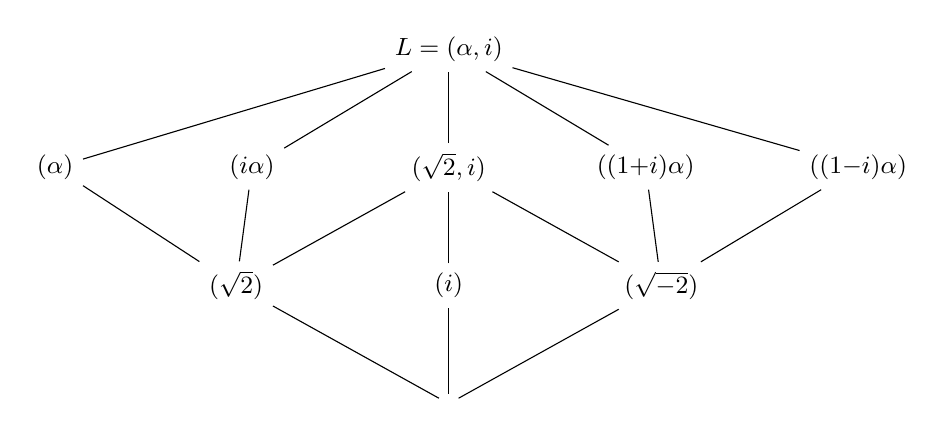
\begin{tikzpicture}[scale=1, every node/.style={font=\small}]
			\node (Q) at (0,0) {$\Q$};
			\node (r2) at (-2.7,1.5) {$\Q(\sqrt2)$};
			\node (i) at (0,1.5) {$\Q(i)$};
			\node (m2) at (2.7,1.5) {$\Q(\sqrt{-2})$};
			\node (A) at (-5.0,3.0) {$\Q(\alpha)$};
			\node (B) at (-2.5,3.0) {$\Q(i\alpha)$};
			\node (C) at (0,3.0) {$\Q(\sqrt2,i)$};
			\node (D) at (2.5,3.0) {$\Q((1{+}i)\alpha)$};
			\node (E) at (5.2,3.0) {$\Q((1{-}i)\alpha)$};
			\node (L) at (0,4.5) {$L = \Q(\alpha,i)$};
			\draw (Q) -- (r2); \draw (Q) -- (i); \draw (Q) -- (m2);
			\draw (r2) -- (A); \draw (r2) -- (B); \draw (r2) -- (C);
			\draw (i) -- (C);
			\draw (m2) -- (C); \draw (m2) -- (D); \draw (m2) -- (E);
			\draw (A) -- (L); \draw (B) -- (L); \draw (C) -- (L);
			\draw (D) -- (L); \draw (E) -- (L);
		\end{tikzpicture}
	\end{center}

	\begin{center}
		\begin{tikzpicture}[scale=1, every node/.style={font=\small}]
			\node (Q) at (0,0) {$D_8$};
			\node (r2) at (-2.7,1.5) {$\langle r^2, s\rangle$};
			\node (i) at (0,1.5) {$\langle r\rangle$};
			\node (m2) at (2.7,1.5) {$\langle r^2, rs\rangle$};
			\node (A) at (-5.0,3.0) {$\langle s\rangle$};
			\node (B) at (-2.5,3.0) {$\langle r^2 s\rangle$};
			\node (C) at (0,3.0) {$\langle r^2\rangle$};
			\node (D) at (2.5,3.0) {$\langle rs\rangle$};
			\node (E) at (5.0,3.0) {$\langle r^3 s\rangle$};
			\node (L) at (0,4.5) {$\{1\}$};
			\draw (Q) -- (r2); \draw (Q) -- (i); \draw (Q) -- (m2);
			\draw (r2) -- (A); \draw (r2) -- (B); \draw (r2) -- (C);
			\draw (i) -- (C);
			\draw (m2) -- (C); \draw (m2) -- (D); \draw (m2) -- (E);
			\draw (A) -- (L); \draw (B) -- (L); \draw (C) -- (L);
			\draw (D) -- (L); \draw (E) -- (L);
		\end{tikzpicture}
	\end{center}

	Reading off part (iii) of the fundamental theorem: the normal subgroups of $D_8$ are $\{1\}$, $\langle r^2\rangle$, the three subgroups of index $2$, and $D_8$ itself. Correspondingly, the subfields Galois over $\Q$ are exactly
	$$\Q, \quad \Q(\sqrt2),\quad \Q(i),\quad \Q(\sqrt{-2}),\quad \Q(\sqrt2,i), \quad L,$$
	and the four degree-$4$ fields $\Q(\alpha), \Q(i\alpha), \Q((1\pm i)\alpha)$ are \emph{not} normal over $\Q$ -- as we can see directly, since for instance $x^4-2$ has only two of its four roots inside $\Q(\alpha)$. Note also that $\langle s\rangle$ and $\langle r^2 s\rangle$ are conjugate in $D_8$ (indeed $r\langle s\rangle r^{-1} = \langle r^2s\rangle$), which matches the fact that $\Q(\alpha)$ and $\Q(i\alpha)$ are abstractly isomorphic fields sitting differently inside $L$.
\end{example}

This example repays study. Almost every phenomenon in the subject is visible in it: non-normal intermediate fields, conjugate subgroups giving isomorphic-but-distinct subfields, and the way that a single degree-$8$ extension can hide ten different fields.

\section{Galois Groups of Polynomials}\label{sec:polys}

We now return to Galois' original setting: a polynomial and the permutations of its roots.

\begin{definition}[Galois Group of a Polynomial]
	Let $f \in K[x]$ be a separable polynomial and let $L$ be a splitting field for $f$ over $K$. Then $L/K$ is Galois, and we write
	$$\Gal(f/K) = \Gal(L/K).$$
	If $f$ has roots $\alpha_1, \dots, \alpha_n$ in $L$, then by Lemma \ref{lem:autbasic} we may regard $\Gal(f/K) \leq S_n$ as a group of permutations of the roots.
\end{definition}

The identification with a subgroup of $S_n$ depends on the ordering of the roots; changing the ordering conjugates the subgroup. So $\Gal(f/K)$ is well defined as a subgroup of $S_n$ only up to conjugacy, which is all we shall ever need.

\begin{proposition}\label{prop:transitive}
	Let $f \in K[x]$ be separable of degree $n$. Then $f$ is irreducible over $K$ if and only if $\Gal(f/K)$ acts transitively on the roots of $f$.
\end{proposition}

\begin{proof}
	Suppose $f$ is irreducible and let $\alpha, \beta$ be roots. By Corollary \ref{cor:sameminpoly} there is a $K$-isomorphism $K(\alpha) \to K(\beta)$ with $\alpha \mapsto \beta$, and by Theorem \ref{thm:splituniq}(i) it extends to $\sigma : L \to L$, which is an automorphism. So the action is transitive.

	Conversely if $f = gh$ non-trivially, then no automorphism can carry a root of $g$ to a root of $h$, by Lemma \ref{lem:autbasic}(i), so the action is not transitive.
\end{proof}

\subsection{Symmetric Polynomials}

The coefficients of a polynomial are symmetric functions of its roots, so any expression in the roots that is invariant under all permutations ought to be expressible in the coefficients. That vague statement has a clean and useful theorem behind it.

Let $R$ be a ring, and let $S_n$ act on $R[z_1,\dots,z_n]$ by permuting the variables, $w \cdot z_i = z_{w(i)}$. The invariant ring $R[z_1,\dots,z_n]^{S_n}$ consists of the \vocab{symmetric polynomials}. Among them are the \vocab{elementary symmetric polynomials}
$$e_1 = \sum_i z_i, \qquad e_2 = \sum_{i<j}z_iz_j, \qquad \dots, \qquad e_n = z_1z_2\cdots z_n.$$

\begin{theorem}[Fundamental Theorem of Symmetric Polynomials]\label{thm:symm}
	The ring homomorphism
	$$R[w_1,\dots,w_n] \to R[z_1,\dots,z_n]^{S_n}, \qquad w_i \mapsto e_i$$
	is an isomorphism. That is, every symmetric polynomial is a polynomial in $e_1,\dots,e_n$, uniquely so.
\end{theorem}

\begin{proof}
	For $\lambda = (\lambda_1,\dots,\lambda_n) \in \N^n$ write $z^\lambda = z_1^{\lambda_1}\cdots z_n^{\lambda_n}$; these monomials form an $R$-basis of $R[z_1,\dots,z_n]$. Order $\N^n$ lexicographically. If $\lambda$ is \emph{decreasing}, meaning $\lambda_1 \geq \lambda_2 \geq \dots \geq \lambda_n$, then $\lambda \geq w\lambda$ for all $w \in S_n$, so every $S_n$-orbit in $\N^n$ contains a unique decreasing element, which is its maximum. It follows that the orbit sums $\sum_{\mu \in S_n\lambda} z^\mu$, indexed by decreasing $\lambda$, form an $R$-basis of the ring of symmetric polynomials.

	\emph{Surjectivity.} Let $f$ be symmetric and non-zero, and let $z^\lambda$ be its lexicographically largest monomial, with coefficient $c$; by symmetry $\lambda$ is decreasing. Consider
	$$E_\lambda = e_1^{\lambda_1-\lambda_2}e_2^{\lambda_2-\lambda_3}\cdots e_{n-1}^{\lambda_{n-1}-\lambda_n}e_n^{\lambda_n}.$$
	Expanding, the lexicographically largest monomial of $e_k$ is $z_1z_2\cdots z_k$, so the lexicographically largest monomial of $E_\lambda$ is
	$$z_1^{\lambda_1-\lambda_2}(z_1z_2)^{\lambda_2-\lambda_3}\cdots(z_1\cdots z_n)^{\lambda_n} = z^\lambda.$$
	Hence $f - cE_\lambda$ is symmetric with strictly smaller leading monomial, and the process terminates by induction (there are finitely many monomials of any given degree).

	\emph{Injectivity.} We induct on $n$; for $n=1$ there is nothing to prove. Suppose $g \in R[w_1,\dots,w_n]$ is non-zero of minimal degree with $g(e_1,\dots,e_n) = 0$. Setting $z_n = 0$ turns $e_i$ into the $i$th elementary symmetric polynomial in $z_1,\dots,z_{n-1}$ for $i < n$, and turns $e_n$ into $0$. So
	$$g(e_1', \dots, e_{n-1}', 0) = 0 \text{ in } R[z_1,\dots,z_{n-1}],$$
	whence by induction $g(w_1,\dots,w_{n-1},0) = 0$ identically, so $w_n \mid g$, say $g = w_n h$. Then $e_n h(e_1,\dots,e_n) = 0$, and $e_n = z_1\cdots z_n \neq 0$ in the integral domain $R[z_1,\dots,z_n]$ (if $R$ is a domain; in general compare coefficients), so $h(e_1,\dots,e_n) = 0$ with $\deg h < \deg g$, contradicting minimality.
\end{proof}

Now let $f \in K[x]$ be monic of degree $n$ with roots $\alpha_1, \dots, \alpha_n$ in a splitting field, so that
$$f(x) = x^n - a_1x^{n-1} + a_2x^{n-2} - \dots + (-1)^n a_n$$
with $a_i = e_i(\alpha_1,\dots,\alpha_n)$. The theorem says that \emph{any} symmetric expression in the roots is a polynomial in the coefficients $a_1,\dots,a_n$, with the same coefficient ring. This is the machine we now use.

\subsection{The Discriminant}

\begin{definition}[Discriminant]
	Let $f \in K[x]$ be monic of degree $n$ with roots $\alpha_1,\dots,\alpha_n$ in a splitting field. The \vocab{discriminant} of $f$ is
	$$\Disc(f) = \prod_{i<j}(\alpha_i - \alpha_j)^2.$$
	We also write $\delta = \prod_{i<j}(\alpha_i - \alpha_j)$, so that $\Disc(f) = \delta^2$.
\end{definition}

\begin{proposition}\label{prop:disc}
	With notation as above, and assuming $\charr K \neq 2$:
	\begin{enumerate}[label=(\roman*)]
		\item $\Disc(f) \in K$, and indeed $\Disc(f)$ is a universal polynomial with integer coefficients in the coefficients of $f$;
		\item $\Disc(f) \neq 0$ if and only if $f$ is separable;
		\item if $f$ is separable, then $\Gal(f/K) \leq A_n$ if and only if $\Disc(f)$ is a square in $K$.
	\end{enumerate}
\end{proposition}

\begin{proof}
	(i) $\Disc(f)$ is a symmetric polynomial in $\alpha_1, \dots, \alpha_n$ with integer coefficients, so by Theorem \ref{thm:symm} it is a polynomial with integer coefficients in $e_1, \dots, e_n$, that is in the coefficients of $f$.

	(ii) is immediate, as $\Disc(f) = 0$ if and only if two roots coincide.

	(iii) Let $G = \Gal(f/K) \leq S_n$. Any $\sigma \in G$ permutes the $\alpha_i$ and hence permutes the factors $(\alpha_i - \alpha_j)$ up to sign, with the sign being $\sign(\sigma)$; that is,
	$$\sigma(\delta) = \sign(\sigma)\delta.$$
	So $G \leq A_n$ if and only if $\sigma\delta = \delta$ for all $\sigma \in G$, which by the Galois correspondence holds if and only if $\delta \in L^G = K$, that is, if and only if $\Disc(f) = \delta^2$ is a square in $K$. (We used $\charr K \neq 2$ to know that $\delta \neq -\delta$.)
\end{proof}

There is a slicker formula for the discriminant in terms of the derivative, which is often the quickest way to compute it.

\begin{proposition}\label{prop:discderiv}
	Let $f$ be monic of degree $n$ with roots $\alpha_1,\dots,\alpha_n$. Then
	$$\prod_{i=1}^n f'(\alpha_i) = (-1)^{n(n-1)/2}\Disc(f).$$
\end{proposition}

\begin{proof}
	Differentiating $f(x) = \prod_j (x-\alpha_j)$ by the product rule gives
	$$f'(x) = \sum_i \prod_{j\neq i}(x-\alpha_j),$$
	and evaluating at $\alpha_i$ kills all the terms but one:
	$$f'(\alpha_i) = \prod_{j \neq i}(\alpha_i - \alpha_j).$$
	Multiplying over $i$ gives $\prod_{i\neq j}(\alpha_i-\alpha_j)$. Pairing off $(i,j)$ with $(j,i)$ introduces a factor $(-1)$ for each of the $\binom{n}{2}$ pairs, giving $(-1)^{n(n-1)/2}\prod_{i<j}(\alpha_i-\alpha_j)^2$.
\end{proof}

\begin{example}
	For a quadratic $f = x^2+bx+c$ we have $\Disc(f) = (\alpha_1-\alpha_2)^2 = (\alpha_1+\alpha_2)^2 - 4\alpha_1\alpha_2 = b^2-4c$, as it should be. Then $\Gal(f/K) \leq A_2 = 1$ if and only if $b^2-4c$ is a square, which is exactly the condition for the roots to lie in $K$.
\end{example}

\begin{example}\label{ex:disccubic}
	For a cubic $f = x^3 + px + q$ we claim
	$$\Disc(f) = -4p^3 - 27q^2.$$
	One can get this cheaply. Since $e_1 = 0$, the discriminant is a polynomial in $e_2 = p$ and $e_3 = -q$ only; and $\Disc$ is homogeneous of degree $6$ in the roots, while $p$ has degree $2$ and $q$ degree $3$, so
	$$\Disc(f) = cp^3 + dq^2$$
	for some integers $c,d$. Taking $f = (x-\alpha)^2(x+2\alpha)$, which has $p = -3\alpha^2$, $q = 2\alpha^3$ and discriminant $0$, gives $-27c\alpha^6 + 4d\alpha^6 = 0$, so $4d = 27c$. Taking $f = x^3 - x$, with roots $0, \pm1$, gives $\Disc = (0-1)^2(0+1)^2(1+1)^2 = 4$, so $-c = 4$; hence $c = -4$ and $d = -27$.
\end{example}

\subsection{Cubics}

Let $f \in K[x]$ be a separable cubic with $\charr K \neq 2, 3$; after substituting $x \mapsto x - a_1/3$ we may take $f = x^3+px+q$. Let $L$ be a splitting field and $G = \Gal(f/K) \leq S_3$.

If $f$ is reducible then $G$ is trivial (three roots in $K$) or $\cong S_2$ (one root in $K$ and an irreducible quadratic factor). So suppose $f$ is irreducible. Then $G$ acts transitively on three points, so $3 \mid \#G$, forcing $G = A_3$ or $G = S_3$; and by Proposition \ref{prop:disc}, $G = A_3$ exactly when $\Disc(f) = -4p^3-27q^2$ is a square in $K$.

The Galois correspondence for the intermediate field $K(\delta) = K(\sqrt{\Disc f})$ then reads as follows.

\begin{center}
	\begin{tikzpicture}[scale=1, every node/.style={font=\small}]
		\node (K) at (0,0) {$K$};
		\node (Kd) at (0,1.6) {$K(\delta) = L^{G \cap A_3}$};
		\node (L) at (0,3.2) {$L = K(\alpha_1,\alpha_2,\alpha_3)$};
		\draw (K) -- node[left=2pt] {$1$ or $2$} (Kd);
		\draw (Kd) -- node[left=2pt] {$3$} (L);
		\node (G) at (5.6,0) {$G$};
		\node (GA) at (5.6,1.6) {$G \cap A_3$};
		\node (one) at (5.6,3.2) {$\{1\}$};
		\draw (G) -- node[right=2pt] {index $1$ or $2$} (GA);
		\draw (GA) -- node[right=2pt] {index $3$} (one);
		\draw[<->, dashed, gray] (3.0,0) -- (4.2,0);
		\draw[<->, dashed, gray] (3.0,1.6) -- (4.2,1.6);
		\draw[<->, dashed, gray] (3.0,3.2) -- (4.2,3.2);
	\end{tikzpicture}
\end{center}

So the splitting field of an irreducible cubic is obtained from $K$ by first adjoining a square root (of the discriminant) and then a cube root -- which is exactly the shape of Cardano's formula. Let us see the cube root appear.

\begin{example}\label{ex:cubicresolvent}
	Suppose $f = x^3+px+q$ is irreducible over $K$, that $\charr K \neq 2,3$, and that $K$ contains $\delta = \sqrt{\Disc f}$ and a primitive cube root of unity $\omega$. Then $G = \Gal(L/K) = A_3 = \langle\sigma\rangle \cong \Z/3$, where we may take $\sigma$ to be the $3$-cycle $\alpha_1 \to \alpha_2 \to \alpha_3 \to \alpha_1$. Define the \vocab{Lagrange resolvents}
	$$\beta = \alpha_1 + \omega\alpha_2+\omega^2\alpha_3, \qquad \gamma = \alpha_1+\omega^2\alpha_2+\omega\alpha_3.$$
	Then $\sigma\beta = \alpha_2 + \omega\alpha_3 + \omega^2\alpha_1 = \omega^{-1}\beta$ and similarly $\sigma\gamma = \omega\gamma$, so $\sigma(\beta^3) = \beta^3$ and $\sigma(\gamma^3) = \gamma^3$; hence $\beta^3, \gamma^3 \in L^G = K$. Also $\alpha_1+\alpha_2+\alpha_3 = 0$, so
	$$\alpha_1 = \tfrac13(\beta+\gamma), \qquad \alpha_2 = \tfrac13(\omega^2\beta+\omega\gamma), \qquad \alpha_3 = \tfrac13(\omega\beta+\omega^2\gamma).$$
	It remains to compute $\beta^3$ and $\gamma^3$. Using $\sum\alpha_i = 0$, $\sum_{i<j}\alpha_i\alpha_j = p$ and $1 + \omega + \omega^2 = 0$:
	$$\beta\gamma = \sum_i \alpha_i^2 + (\omega+\omega^2)\sum_{i<j}\alpha_i\alpha_j = \left(\sum_i\alpha_i\right)^2 - 3\sum_{i<j}\alpha_i\alpha_j = -3p,$$
	so $\beta^3\gamma^3 = -27p^3$. A similar (slightly longer) expansion gives $\beta^3 + \gamma^3 = -27q$. Hence $\beta^3, \gamma^3$ are the roots of
	$$t^2 + 27qt - 27p^3 = 0,$$
	that is $\beta^3 = \tfrac12(-27q + 3\sqrt{-3\Disc f})$, and then $\gamma = -3p/\beta$. This is Cardano's formula, derived rather than guessed.
\end{example}

\subsection{Quartics and the Resolvent Cubic}

Now let $f \in K[x]$ be an irreducible separable quartic, with $\charr K \neq 2,3$, splitting field $L$ and $G = \Gal(f/K) \leq S_4$. Translating, we may assume $\sum\alpha_i = 0$, so
$$f(x) = x^4 + px^2 + qx + r.$$

Since $G$ is transitive, $4 \mid \#G$, and the transitive subgroups of $S_4$ are (up to conjugacy)
$$S_4, \quad A_4, \quad D_8 = \langle (1234), (13)\rangle, \quad \Z/4 = \langle(1234)\rangle,$$
$$V = \{e,(12)(34),(13)(24),(14)(23)\}.$$
The key structural fact is that the Klein four-group $V$ is normal in $S_4$, with $S_4/V \cong S_3$; concretely, $S_4$ acts on the three partitions
$$(12\mid34), \qquad (13\mid24), \qquad (14\mid23)$$
of $\{1,2,3,4\}$ into two pairs, and the kernel of the resulting homomorphism $S_4 \to S_3$ is exactly $V$. Since $\#V \cdot \#S_3 = 24$, the map is surjective.

Under the Galois correspondence, $G \cap V \normal G$ corresponds to an intermediate field $M = L^{G\cap V}$ with $\Gal(M/K) = G/(G\cap V) \hookrightarrow S_4/V \cong S_3$. So $M$ should be the splitting field of a \emph{cubic}, and we can find it.

Put
$$y_{12} = \alpha_1+\alpha_2 = -(\alpha_3+\alpha_4) = -y_{34},$$
and similarly $y_{13}, y_{14}$. Each element of $V$ either fixes $y_{12}$ or sends it to $y_{34} = -y_{12}$, so $y_{12}^2, y_{13}^2, y_{14}^2$ are fixed by $V$ and hence lie in $M$. They are distinct: if $y_{12}^2 = y_{13}^2$ then either $y_{12} = y_{13}$, giving $\alpha_2 = \alpha_3$, or $y_{12} = -y_{13}$, giving $2\alpha_1 + \alpha_2+\alpha_3 = 0$ and hence $\alpha_1 = \alpha_4$; both contradict separability. Finally $S_4$ permutes $\{y_{12}^2, y_{13}^2, y_{14}^2\}$, so their elementary symmetric functions lie in $K$.

\begin{definition}[Resolvent Cubic]
	The \vocab{resolvent cubic} of $f = x^4+px^2+qx+r$ is
	$$g(x) = (x - y_{12}^2)(x-y_{13}^2)(x-y_{14}^2) \in K[x].$$
\end{definition}

\begin{proposition}
	With notation as above, $g(x) = x^3 + 2px^2 + (p^2-4r)x - q^2$, and $M = L^{G\cap V}$ is a splitting field for $g$ over $K$. Moreover $L = M(y_{12}, y_{13})$, and $\alpha_1 = \tfrac12(y_{12}+y_{13}+y_{14})$ with $y_{12}y_{13}y_{14} = -q$.
\end{proposition}

\begin{proof}
	The formula for $g$ is a direct expansion using the symmetric function identities $\sum\alpha_i = 0$, $\sum_{i<j}\alpha_i\alpha_j = p$, $\sum_{i<j<k}\alpha_i\alpha_j\alpha_k = -q$, $\alpha_1\alpha_2\alpha_3\alpha_4 = r$; for instance
	$$y_{12}^2+y_{13}^2+y_{14}^2 = -\big((\alpha_1+\alpha_2)(\alpha_3+\alpha_4)+\dots\big) = -2p.$$
	That $M \supseteq K(y_{12}^2,y_{13}^2,y_{14}^2)$ we have already seen; equality follows from Artin's theorem, since $\aut(L/K(y_{12}^2,y_{13}^2,y_{14}^2)) = G\cap V$ (an automorphism fixing all three squares must preserve each partition, hence lie in $V$).

	For the last statements, $\alpha_1 = \frac12\big((\alpha_1+\alpha_2)+(\alpha_1+\alpha_3)+(\alpha_1+\alpha_4)\big)$ since $\sum\alpha_i = 0$, and $y_{12}y_{13}y_{14} = -q$ by another expansion. Hence $L = K(\alpha_1,\dots,\alpha_4) = M(y_{12},y_{13},y_{14}) = M(y_{12},y_{13})$.
\end{proof}

So a quartic is solved by first solving its resolvent cubic and then extracting two square roots -- and the whole tower is
$$K \subseteq K(\delta) \subseteq M \subseteq L$$
of degrees dividing $2, 3, 4$ respectively. Comparing $G$ with $G \cap A_4$ and $G \cap V$ lets us determine $G$ completely.

\begin{proposition}
	Let $f$ be an irreducible separable quartic over $K$ with resolvent cubic $g$. Then $\Gal(f/K)$ is determined by the following table, where $\delta = \sqrt{\Disc f}$.
	\begin{center}
		\begin{tabular}{lll}
			\hline
			$g$ irreducible over $K$? & $\delta \in K$? & $G$ \\
			\hline
			yes & yes & $A_4$ \\
			yes & no & $S_4$ \\
			no, splits completely & yes & $V$ \\
			no, one root in $K$ & no & $D_8$ or $\Z/4$ \\
			\hline
		\end{tabular}
	\end{center}
\end{proposition}

\begin{proof}
	We have $[M:K] = \#(G/(G\cap V))$, which is the order of the image of $G$ in $S_3$, and this image is $\Gal(g/K)$. Also $\delta \in K$ if and only if $G \leq A_4$. Running through the five transitive subgroups: $G = S_4$ gives image $S_3$ and $\delta\notin K$; $G = A_4$ gives image $A_3$ (so $g$ is irreducible) and $\delta \in K$; $G = V$ gives trivial image, so $g$ splits, and $V \leq A_4$ so $\delta\in K$; $G = D_8$ or $\Z/4$ gives image of order $2$, so $g$ has exactly one root in $K$, and neither is contained in $A_4$.
\end{proof}

Distinguishing $D_8$ from $\Z/4$ requires slightly more work (one asks whether $f$ remains irreducible over $K(\delta)$), and we shall not pursue it.

\subsection{Reduction Modulo a Prime}

For polynomials over $\Z$ there is a beautiful and very practical technique: reduce mod $p$, where finite field theory tells us everything, and transfer the information back.

Recall from Example \ref{ex:frobgen} that $\Gal(\overline f/\F_p)$ is cyclic, generated by Frobenius. Its cycle type is easy to read off.

\begin{proposition}\label{prop:fpcycle}
	Let $\overline f \in \F_p[x]$ be separable of degree $n$ with irreducible factors of degrees $n_1, \dots, n_r$. Then $\Gal(\overline f/\F_p)$ is cyclic, generated by an element of cycle type $(n_1,\dots,n_r)$, and so has order $\lcm(n_1,\dots,n_r)$.
\end{proposition}

\begin{proof}
	Let $L$ be a splitting field. Then $\Gal(L/\F_p) = \langle\varphi\rangle$ with $\varphi(x) = x^p$. If $\alpha$ is a root of the irreducible factor $g_i$, then the roots of $g_i$ are exactly the $\varphi$-orbit of $\alpha$, which therefore has size $\deg g_i = n_i$. So $\varphi$ acts on the $n$ roots as a product of disjoint cycles of lengths $n_1,\dots,n_r$.
\end{proof}

\begin{theorem}[Dedekind]\label{thm:dedekind}
	Let $f \in \Z[x]$ be monic and separable of degree $n$, and let $p$ be a prime such that the reduction $\overline f \in \F_p[x]$ is also separable. Then $\Gal(\overline f/\F_p)$ is (conjugate in $S_n$ to) a subgroup of $\Gal(f/\Q)$.
\end{theorem}

\begin{proof}[Proof sketch]
	Let $L$ be a splitting field for $f$ over $\Q$, with roots $\alpha_1,\dots,\alpha_n$, and put $R = \Z[\alpha_1,\dots,\alpha_n]$. Since $f$ is monic, $R$ is finitely generated as a $\Z$-module. It is torsion-free, so it is free, say $R \cong \Z^M$. Choose a maximal ideal $P \supseteq pR$ of $R$; then $F = R/P$ is a finite field of characteristic $p$, generated by the images $\overline\alpha_i$, and in $F[x]$ we have
	$$\overline f = \prod_i (x - \overline\alpha_i).$$ As $\overline f$ is separable the $\overline\alpha_i$ are distinct, so $F$ is a splitting field for $\overline f$.

	The group $G = \Gal(f/\Q)$ permutes the $\alpha_i$ and hence acts on $R$; let $H = \stab_G(P)$. Then $H$ acts on $F = R/P$, permuting the $\overline\alpha_i$ exactly as it permutes the $\alpha_i$, giving an injection $H \hookrightarrow \Gal(F/\F_p)$. A counting argument using the Chinese remainder theorem on the $G$-orbit of $P$ shows this injection is onto, which gives the result.
\end{proof}

\begin{corollary}\label{cor:dedekind}
	With $f$ and $p$ as above, if $\overline f$ factors into distinct irreducibles of degrees $n_1,\dots,n_r$ over $\F_p$, then $\Gal(f/\Q)$ contains a permutation of cycle type $(n_1,\dots,n_r)$.
\end{corollary}

\begin{example}
	Let $f = x^4 - 3x+1$.
	\begin{itemize}
		\item Mod $2$: $\overline f = x^4+x+1$, which has no root in $\F_2$ and is not divisible by $x^2+x+1$ (the only irreducible quadratic), so it is irreducible. Hence $\Gal(f/\Q)$ contains a $4$-cycle.
		\item Mod $5$: $\overline f = (x+1)(x^3-x^2+x+1)$, a product of an irreducible linear and an irreducible cubic. Hence $\Gal(f/\Q)$ contains a $3$-cycle.
	\end{itemize}
	So $12 \mid \#\Gal(f/\Q)$, and $\Gal(f/\Q) \leq S_4$, so it is $A_4$ or $S_4$. But a $4$-cycle is odd, so it is not in $A_4$. Hence $\Gal(f/\Q) = S_4$.
\end{example}

Note also that reduction mod $p$ is a good irreducibility test: if $\overline f$ is irreducible for some $p$ then $f$ is irreducible over $\Z$ and hence over $\Q$. More subtly, a factorisation over $\Z$ must refine to a factorisation over $\F_p$ for every $p$, so if the factorisation shapes mod two different primes are incompatible, $f$ is irreducible. For example $f = x^4+5x^2-2x-3$ factors as $(x^2+x+1)^2$ mod $2$ and as $x(x^3+2x+1)$ mod $3$; a factorisation over $\Z$ would have to have a factor of degree $2$ (from mod $2$) and a factor of degree $1$ (from mod $3$) compatible with each other, which is impossible, so $f$ is irreducible.

\subsection{The Generic Polynomial}

Finally, symmetric functions let us produce a polynomial whose Galois group is as large as possible.

\begin{theorem}\label{thm:generic}
	Let $k$ be a field and let $L = k(z_1,\dots,z_n)$ be the field of rational functions, with $S_n$ acting by permuting the variables. Then
	$$L^{S_n} = k(e_1,\dots,e_n),$$
	and $L/L^{S_n}$ is a Galois extension of degree $n!$ with Galois group $S_n$.
\end{theorem}

\begin{proof}
	Certainly $k(e_1,\dots,e_n)\subseteq L^{S_n}$. Conversely let $\gamma = f/g \in L^{S_n}$ with $f, g \in R = k[z_1,\dots,z_n]$. Put $\mu = \prod_{\sigma\in S_n}\sigma g$, which is symmetric, so $\mu \in R^{S_n} = k[e_1,\dots,e_n]$ by Theorem \ref{thm:symm}. Then
	$$\gamma = \frac{f}{g} = \frac{f \prod_{\sigma\neq 1}\sigma g}{\mu},$$
	whose numerator is $\gamma\mu$, a symmetric element of $R$ (it is symmetric since $\gamma$ and $\mu$ are, and it lies in $R$). So $\gamma \in \Frac(R^{S_n}) = k(e_1,\dots,e_n)$.

	Since $S_n$ acts faithfully on $L$, Artin's Theorem \ref{thm:artin} gives $[L:L^{S_n}] = n!$ with $\Gal(L/L^{S_n}) = S_n$.
\end{proof}

Taking $K = k(e_1,\dots,e_n)$ and $f(x) = x^n - e_1x^{n-1}+\dots+(-1)^ne_n \in K[x]$, we have $f(x) = \prod_i (x - z_i)$ in $L$, so $L$ is a splitting field for $f$ and
$$\Gal(f/K) = S_n.$$
Informally: \emph{the general polynomial of degree $n$ has Galois group $S_n$}. This will be exactly what we need for the insolubility of the quintic.

\begin{corollary}
	Every finite group $G$ occurs as the Galois group of some Galois extension of fields.
\end{corollary}

\begin{proof}
	By Cayley's theorem $G$ embeds in $S_n$ for some $n$ (acting on itself by left multiplication). Take $L = k(z_1,\dots,z_n)$ and apply Artin's theorem to $G \leq S_n \leq \aut(L)$: then $L/L^G$ is Galois with group $G$.
\end{proof}

Whether every finite group occurs as $\Gal(L/\Q)$ is the \vocab{inverse Galois problem}, and it is open. It is known for all soluble groups (Shafarevich) and for most finite simple groups, including -- thanks to Thompson -- the Monster.

\section{Cyclotomic Extensions}\label{sec:cyclotomic}

We now study the extension obtained by adjoining roots of unity. These are the simplest interesting Galois extensions of $\Q$, and they are also the raw material out of which radical extensions are built, so we shall need to understand them thoroughly.

\subsection{Roots of Unity}

Let $K$ be a field and $n \geq 1$ with $n \neq 0$ in $K$ (so $\charr K = 0$, or $\charr K = p \nmid n$). Then $x^n - 1$ has derivative $nx^{n-1}$, and $\gcd(x^n-1, nx^{n-1}) = 1$, so $x^n-1$ is separable. Let $L$ be a splitting field and
$$\mu_n = \{\zeta \in L : \zeta^n = 1\},$$
a group of order exactly $n$ under multiplication. By Proposition \ref{prop:cyclic} it is cyclic.

\begin{definition}[Primitive Root of Unity]
	A generator of $\mu_n$ is called a \vocab{primitive $n$th root of unity}, usually written $\zeta_n$. There are $\phi(n)$ of them, namely $\zeta_n^a$ for $\gcd(a,n)=1$.
\end{definition}

Over $\C$ we can draw the picture: the $n$th roots of unity are the vertices of a regular $n$-gon inscribed in the unit circle, and the primitive ones are those `visible from the origin' in the sense of being $e^{2\pi i a/n}$ with $a$ coprime to $n$. Here is $n = 12$, with the four primitive twelfth roots of unity drawn as solid dots.

\begin{center}
	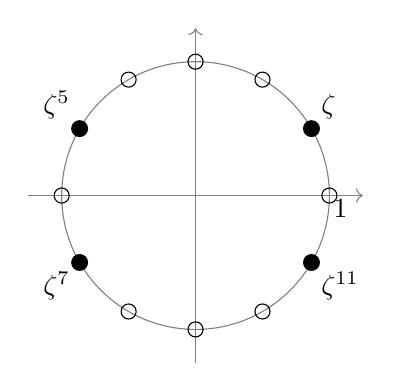
\begin{tikzpicture}[scale=1.7]
		\draw[thin, gray] (0,0) circle (1);
		\draw[->, thin, gray] (-1.25,0) -- (1.25,0);
		\draw[->, thin, gray] (0,-1.25) -- (0,1.25);
		\foreach \k in {0,2,3,4,6,8,9,10} {
			\draw ({cos(30*\k)},{sin(30*\k)}) circle (1.6pt);
		}
		\foreach \k in {1,5,7,11} {
			\fill ({cos(30*\k)},{sin(30*\k)}) circle (1.8pt);
		}
		\node[below right=-2pt] at (1,0) {$1$};
		\node[above right] at ({cos(30)},{sin(30)}) {$\zeta$};
		\node[above left] at ({cos(150)},{sin(150)}) {$\zeta^5$};
		\node[below left] at ({cos(210)},{sin(210)}) {$\zeta^7$};
		\node[below right] at ({cos(330)},{sin(330)}) {$\zeta^{11}$};
	\end{tikzpicture}
\end{center}

\begin{proposition}\label{prop:cycgalois}
	Let $\zeta = \zeta_n$ be a primitive $n$th root of unity in a splitting field $L$ of $x^n-1$ over $K$. Then $L = K(\zeta)$, the extension $L/K$ is Galois, and there is an injective group homomorphism
	$$\chi : \Gal(L/K) \hookrightarrow (\Z/n\Z)^\times.$$
	In particular $\Gal(L/K)$ is abelian.
\end{proposition}

\begin{proof}
	Every $n$th root of unity is a power of $\zeta$, so $L = K(\zeta)$; and $L$ is the splitting field of the separable polynomial $x^n-1$, so $L/K$ is Galois. Any $\sigma \in \Gal(L/K)$ sends $\zeta$ to another root of $x^n-1$, and must send a generator of $\mu_n$ to a generator, so $\sigma(\zeta) = \zeta^{a_\sigma}$ for a unique $a_\sigma \in (\Z/n\Z)^\times$. If $\tau(\zeta) = \zeta^{a_\tau}$ then
	$$\sigma\tau(\zeta) = \sigma(\zeta^{a_\tau}) = \zeta^{a_\sigma a_\tau},$$
	so $\chi(\sigma) = a_\sigma$ is a homomorphism, and it is injective since $\sigma$ is determined by $\sigma(\zeta)$.
\end{proof}

For general $K$ the map $\chi$ need not be surjective -- for instance if $K$ already contains $\zeta$ then $\Gal(L/K)$ is trivial. The whole content of the next subsection is that over $\Q$ it \emph{is} surjective.

\subsection{Cyclotomic Polynomials}

If $d \mid n$ then $x^d - 1$ divides $x^n-1$. Each $\zeta \in \mu_n$ is a primitive $d$th root of unity for exactly one $d \mid n$, namely $d = \ord(\zeta)$. This suggests dividing out all the obvious factors.

\begin{definition}[Cyclotomic Polynomial]
	The $n$th \vocab{cyclotomic polynomial} is
	$$\Phi_n(x) = \prod_{\substack{\zeta \in \mu_n \\ \ord(\zeta) = n}} (x - \zeta) = \prod_{\substack{1 \leq a \leq n\\ \gcd(a,n)=1}}(x - \zeta_n^a),$$
	a monic polynomial of degree $\phi(n)$.
\end{definition}

Partitioning $\mu_n$ by the order of its elements gives
$$x^n - 1 = \prod_{d \mid n}\Phi_d(x), \qquad\text{equivalently}\qquad \Phi_n(x) = \frac{x^n-1}{\prod_{d\mid n,\ d\neq n}\Phi_d(x)},$$
which is an inductive recipe for computing $\Phi_n$.

\begin{proposition}
	$\Phi_n(x) \in \Z[x]$.
\end{proposition}

\begin{proof}
	Induct on $n$. For $n=1$, $\Phi_1 = x-1$. In general $g = \prod_{d\mid n, d\neq n}\Phi_d$ lies in $\Z[x]$ by induction and is monic, so dividing $x^n-1$ by $g$ using the division algorithm in $\Z[x]$ (legitimate as $g$ is monic) gives a quotient in $\Z[x]$; and that quotient must be $\Phi_n$, since the division is the same computed in any larger ring.
\end{proof}

\begin{example}
	The first few are $\Phi_1 = x-1$, $\Phi_2 = x+1$, $\Phi_3 = x^2+x+1$, $\Phi_4 = x^2+1$. For $p$ prime, $\Phi_p = 1 + x + \dots + x^{p-1}$. For $n = 8$ and $n=6$:
	\begin{align*}
		x^8-1 &= \underbrace{(x-1)}_{\Phi_1}\underbrace{(x+1)}_{\Phi_2}\underbrace{(x^2+1)}_{\Phi_4}\underbrace{(x^4+1)}_{\Phi_8},\\
		x^6-1 &= \underbrace{(x-1)}_{\Phi_1}\underbrace{(x+1)}_{\Phi_2}\underbrace{(x^2+x+1)}_{\Phi_3}\underbrace{(x^2-x+1)}_{\Phi_6}.
	\end{align*}
	It is tempting to guess that the coefficients of $\Phi_n$ are always $0, \pm1$. This is true for $n < 105$, and false for $n = 105$.
\end{example}

\begin{theorem}[Gauss, Dedekind]\label{thm:phiirred}
	$\Phi_n$ is irreducible in $\Q[x]$.
\end{theorem}

\begin{proof}
	By Gauss's lemma, since $\Phi_n \in \Z[x]$ is monic, it suffices to show $\Phi_n$ does not factor properly in $\Z[x]$. Suppose $\Phi_n = fg$ with $f, g \in \Z[x]$ monic and $f$ irreducible of positive degree.

	Let $\xi$ be a root of $f$; it is a primitive $n$th root of unity, and every primitive $n$th root of unity is $\xi^a$ with $\gcd(a,n)=1$. Since every such $a$ is a product of primes not dividing $n$, it is enough to prove:
	$$\text{if } f(\xi) = 0 \text{ and } p \text{ is a prime with } p \nmid n, \text{ then } f(\xi^p) = 0.$$
	Granting this, every root of $\Phi_n$ is a root of $f$, so $\deg f = \phi(n)$ and $g$ is constant, as required.

	Suppose not, so $f(\xi^p) \neq 0$. Since $\xi^p$ is a primitive $n$th root of unity, $\Phi_n(\xi^p) = 0$, so $g(\xi^p) = 0$. Thus $\xi$ is a root of both $f(x)$ and $g(x^p)$; as $f$ is irreducible and monic it is the minimal polynomial of $\xi$ over $\Q$, so
	$$f(x) \mid g(x^p) \text{ in } \Z[x]$$
	(the quotient lies in $\Z[x]$ by Gauss's lemma, as $f$ is monic).

	Now reduce modulo $p$, writing $\overline h$ for the image of $h$ in $\F_p[x]$. By the Frobenius homomorphism, $\overline g(x^p) = \overline g(x)^p$. So
	$$\overline f \mid \overline g^{\,p} \text{ in } \F_p[x].$$
	Let $\gamma$ be an irreducible factor of $\overline f$; then $\gamma \mid \overline g$, so $\gamma^2 \mid \overline f\, \overline g = \overline{\Phi_n}$, and hence $\overline{\Phi_n}$ has a repeated root. But $\overline{\Phi_n} \mid x^n-1$ in $\F_p[x]$, and $x^n-1$ is separable over $\F_p$ because $p \nmid n$. This is a contradiction.
\end{proof}

\begin{corollary}\label{cor:cycQ}
	$[\Q(\zeta_n):\Q] = \phi(n)$, and
	$$\chi : \Gal(\Q(\zeta_n)/\Q) \xrightarrow{\ \sim\ } (\Z/n\Z)^\times$$
	is an isomorphism.
\end{corollary}

\begin{proof}
	$\Phi_n$ is the minimal polynomial of $\zeta_n$ over $\Q$ by Theorem \ref{thm:phiirred}, so $[\Q(\zeta_n):\Q] = \phi(n) = \#(\Z/n\Z)^\times$. The map $\chi$ of Proposition \ref{prop:cycgalois} is injective between groups of the same finite order, hence bijective.
\end{proof}

\subsection{Subfields of Cyclotomic Fields}

Since $(\Z/n\Z)^\times$ is abelian, every subgroup is normal, so \emph{every} subfield of $\Q(\zeta_n)$ is Galois over $\Q$ with abelian Galois group. (The converse -- that every abelian extension of $\Q$ lies inside a cyclotomic field -- is the Kronecker--Weber theorem, well beyond this course.) The Galois correspondence therefore turns questions about subfields of $\Q(\zeta_n)$ into questions about subgroups of $(\Z/n\Z)^\times$.

\begin{lemma}\label{lem:realsubfield}
	Let $n \geq 3$. Then the fixed field of complex conjugation in $\Q(\zeta_n)$ is the maximal real subfield
	$$\Q(\zeta_n + \zeta_n^{-1}) = \Q(2\cos(2\pi/n)),$$
	and $[\Q(\zeta_n) : \Q(\zeta_n+\zeta_n^{-1})] = 2$. In particular $2 \mid \phi(n)$.
\end{lemma}

\begin{proof}
	Complex conjugation restricts to an element of $\Gal(\Q(\zeta_n)/\Q)$ corresponding to $-1 \in (\Z/n\Z)^\times$, which is not the identity since $n \geq 3$; so it has order $2$ and its fixed field has index $2$. Now $\eta = \zeta+\zeta^{-1} = 2\cos(2\pi/n)$ is real, so $\Q(\eta)$ lies in that fixed field; and $\zeta$ is a root of $x^2 - \eta x + 1 \in \Q(\eta)[x]$, so $[\Q(\zeta):\Q(\eta)]\leq 2$, with equality since $\zeta\notin\R$. Comparing degrees, $\Q(\eta)$ is exactly the fixed field.
\end{proof}

\begin{remark}
	When $\Gal(\Q(\zeta_n)/\Q)$ is not cyclic there may be several subfields of index $2$; for instance $\Q(\zeta_8)$ has degree $4$ over $\Q$ and contains all three of $\Q(i), \Q(\sqrt2)$ and $\Q(\sqrt{-2})$. The maximal real subfield is the one fixed by conjugation, here $\Q(\sqrt 2)$.
\end{remark}

\begin{example}[$n = 5$]
	Here $(\Z/5)^\times \cong \Z/4$, so there is a unique intermediate field of degree $2$ over $\Q$, namely $\Q(\eta)$ with $\eta = \zeta_5 + \zeta_5^{-1}$. Since $\zeta+\zeta^2+\zeta^3+\zeta^4 = -1$, we get $\eta + \eta' = -1$ where $\eta' = \zeta^2+\zeta^3$, and $\eta\eta' = -1$, so $\eta$ satisfies $x^2+x-1$ and
	$$\eta = \frac{-1+\sqrt5}{2}, \qquad \Q\subsetneq \Q(\sqrt5)\subsetneq \Q(\zeta_5).$$
\end{example}

\begin{example}[$n=7$]\label{ex:zeta7}
	Now $(\Z/7)^\times \cong \Z/6$, generated by $3$; write $\sigma = \chi^{-1}(3)$, so $\sigma(\zeta) = \zeta^3$. The subgroups of $\Z/6$ are $\{1\}, \langle\sigma^3\rangle \cong \Z/2, \langle\sigma^2\rangle\cong\Z/3$ and the whole group, so $\Q(\zeta_7)$ has exactly four subfields.

	The subgroup $\langle\sigma^3\rangle$ has order $2$, so its fixed field has degree $3$. Since $\sigma^3(\zeta) = \zeta^{27} = \zeta^{-1}$, this is $\Q(\eta)$ with $\eta = \zeta+\zeta^{-1}$, and the orbit of $\eta$ under $\langle\sigma\rangle$ is $\{\eta_1,\eta_2,\eta_3\}$ where $\eta_j = \zeta^j+\zeta^{-j}$. So the minimal polynomial of $\eta$ is
	$$(x-\eta_1)(x-\eta_2)(x-\eta_3) = x^3+x^2-2x-1.$$

	The subgroup $\langle\sigma^2\rangle$ has order $3$, so its fixed field is quadratic. Put $\varepsilon = \zeta+\zeta^2+\zeta^4$ (the orbit of $\zeta$ under $\langle\sigma^2\rangle$, since $\sigma^2(\zeta) = \zeta^2$). Then $\varepsilon' = \zeta^3+\zeta^5+\zeta^6$ is its conjugate, and
	$$\varepsilon+\varepsilon' = -1, \qquad \varepsilon\varepsilon' = 2,$$
	so $\varepsilon$ satisfies $x^2+x+2$, whose discriminant is $-7$. Hence the quadratic subfield is $\Q(\sqrt{-7})$.
\end{example}

\begin{center}
	\begin{tikzpicture}[scale=1, every node/.style={font=\small}]
		\node (Q) at (0,0) {$\Q$};
		\node (A) at (-1.6,1.5) {$\Q(\sqrt{-7})$};
		\node (B) at (1.6,1.5) {$\Q(\zeta_7+\zeta_7^{-1})$};
		\node (L) at (0,3.0) {$\Q(\zeta_7)$};
		\draw (Q) -- node[left=2pt] {$2$} (A);
		\draw (Q) -- node[right=2pt] {$3$} (B);
		\draw (A) -- node[left=2pt] {$3$} (L);
		\draw (B) -- node[right=2pt] {$2$} (L);
		\node (G) at (6.6,0) {$\Z/6$};
		\node (GA) at (5.0,1.5) {$\langle\sigma^2\rangle$};
		\node (GB) at (8.2,1.5) {$\langle\sigma^3\rangle$};
		\node (one) at (6.6,3.0) {$\{1\}$};
		\draw (G) -- (GA); \draw (G) -- (GB);
		\draw (GA) -- (one); \draw (GB) -- (one);
	\end{tikzpicture}
\end{center}

The pattern in these examples is general.

\begin{proposition}\label{prop:quadsubfield}
	Let $p$ be an odd prime. Then the unique quadratic subfield of $\Q(\zeta_p)$ is $\Q(\sqrt{p^*})$, where
	$$p^* = (-1)^{(p-1)/2}p.$$
\end{proposition}

\begin{proof}
	Since $\Gal(\Q(\zeta_p)/\Q)\cong \Z/(p-1)$ is cyclic of even order, it has a unique subgroup of index $2$, so there is a unique quadratic subfield $F$.

	Now apply Proposition \ref{prop:discderiv} to $f(x) = x^p-1$, whose roots are the $p$th roots of unity and whose derivative is $px^{p-1}$:
	$$\Disc(f) = (-1)^{p(p-1)/2}\prod_{j=0}^{p-1}p\zeta^{j(p-1)} = (-1)^{(p-1)/2}p^p\,\zeta^{(p-1)\cdot\frac{p(p-1)}{2}} = (-1)^{(p-1)/2}p^p,$$
	using that $p$ is odd and $\zeta^{p} = 1$. Since $p$ is odd, $p^p$ and $p$ differ by the square $p^{p-1}$, so
	$$\Q(\sqrt{\Disc f}) = \Q\left(\sqrt{(-1)^{(p-1)/2}p}\right) = \Q(\sqrt{p^*}).$$
	But $\delta = \sqrt{\Disc f}$ lies in the splitting field $\Q(\zeta_p)$ and generates a quadratic extension of $\Q$ (it is irrational since $p^*$ is not a square). By uniqueness, $F = \Q(\sqrt{p^*})$.
\end{proof}

\begin{corollary}
	$\Gal(\Q(\zeta_p)/\Q) \not\leq A_p$, when regarded as permutations of the $p$th roots of unity.
\end{corollary}

This proposition is the first step of one of the standard Galois-theoretic proofs of quadratic reciprocity, which you may have seen in Number Theory.

\subsection{Constructible Polygons}

We can now settle the question left open in Section \ref{sec:construct}.

\begin{theorem}[Gauss]\label{thm:gausspoly}
	The regular $n$-gon is constructible with ruler and compass if and only if
	$$n = 2^k p_1p_2\cdots p_r$$
	where the $p_i$ are distinct primes of the form $2^{2^\ell}+1$.
\end{theorem}

Primes of the form $2^m+1$ are called \vocab{Fermat primes}; note that $m$ must itself be a power of $2$, since if $m$ has an odd factor $t>1$ then $2^{m/t}+1$ divides $2^m+1$. The only known Fermat primes are $3, 5, 17, 257$ and $65537$.

\begin{proof}
	Constructing the regular $n$-gon is equivalent to constructing $\cos(2\pi/n)$, and since $[\Q(\zeta_n) : \Q(\cos(2\pi/n))] = 2$ by Lemma \ref{lem:realsubfield}, this is equivalent to constructing $\zeta_n$, that is, to every element of $\Q(\zeta_n)$ being constructible.

	($\Rightarrow$) If $\zeta_n$ is constructible then by Corollary \ref{cor:construct} its degree over $\Q$ is a power of $2$, that is $\phi(n) = 2^s$. Writing $n = \prod_i p_i^{\alpha_i}$ we have $\phi(n) = \prod_i p_i^{\alpha_i-1}(p_i-1)$, so no odd prime may occur with $\alpha_i \geq 2$, and each odd $p_i$ must have $p_i - 1$ a power of $2$. That is exactly the stated form.

	($\Leftarrow$) Suppose $\phi(n) = 2^s$, so $G = \Gal(\Q(\zeta_n)/\Q)$ is an abelian group of order $2^s$. Any such group has a chain of subgroups
	$$\{1\} = A_0 < A_1 < \dots < A_s = G$$
	with $A_{j}/A_{j-1}\cong \Z/2$ (take a chain through the factors given by the structure theorem, or simply induct: an abelian $2$-group has a subgroup of index $2$). By the Galois correspondence this gives a tower
	$$\Q = F_0 \subset F_1 \subset \dots \subset F_s = \Q(\zeta_n)$$
	with each $[F_j : F_{j-1}] = 2$, so each $F_j = F_{j-1}(\sqrt{r_j})$ for some $r_j \in F_{j-1}$. By Theorem \ref{thm:construct}, everything in $\Q(\zeta_n)$ is constructible.
\end{proof}

\begin{example}[The $17$-gon]
	Here $(\Z/17)^\times \cong \Z/16$, which has the chain $\{1\} < \Z/2 < \Z/4 < \Z/8 < \Z/16$, so
	$$\Q \subset K_1 \subset K_2 \subset K_3 \subset \Q(\zeta_{17})$$
	with each step quadratic, and $K_3 = \Q(\cos(2\pi/17))$. So $\cos(2\pi/17)$ is obtained from $\Q$ by extracting four successive square roots, and the regular $17$-gon is constructible. Gauss discovered this at the age of nineteen, and it is said to have decided him on a career in mathematics.
\end{example}

\section{Kummer Theory and Cyclic Extensions}\label{sec:kummer}

Cyclotomic extensions are the extensions generated by roots of $x^n-1$. We now consider the general $x^n - a$, and discover that -- once enough roots of unity are present -- these are exactly the cyclic extensions. This is the last piece of machinery we need for the insolubility of the quintic.

\subsection{Linear Independence of Characters}

\begin{theorem}[Dedekind, Artin]\label{thm:linind}
	Let $G$ be a group, $L$ a field, and $\sigma_1, \dots, \sigma_n : G \to L^\times$ distinct group homomorphisms. Then $\sigma_1,\dots,\sigma_n$ are linearly independent over $L$ as functions $G \to L$.
\end{theorem}

\begin{proof}
	Induct on $n$; the case $n = 1$ is clear since $\sigma_1$ is nowhere zero. Suppose $y_1, \dots, y_n \in L$ satisfy
	$$y_1\sigma_1(g) + \dots + y_n\sigma_n(g) = 0 \quad\text{for all } g \in G. \qquad (\ast)$$
	As $\sigma_1 \neq \sigma_n$, choose $h \in G$ with $\sigma_1(h)\neq\sigma_n(h)$. Substituting $hg$ for $g$ in $(\ast)$ and using multiplicativity,
	$$y_1\sigma_1(h)\sigma_1(g)+\dots+y_n\sigma_n(h)\sigma_n(g) = 0.$$
	Subtracting $\sigma_n(h)$ times $(\ast)$ kills the last term:
	$$\sum_{i=1}^{n-1}y_i\big(\sigma_i(h)-\sigma_n(h)\big)\sigma_i(g) = 0 \quad\text{for all }g.$$
	By induction all the coefficients vanish; in particular $y_1(\sigma_1(h)-\sigma_n(h)) = 0$, so $y_1 = 0$. Now $(\ast)$ has only $n-1$ terms, and induction finishes the job.
\end{proof}

\begin{corollary}[Linear independence of embeddings]\label{cor:linind}
	Let $K, L$ be fields and $\sigma_1,\dots,\sigma_n : K \to L$ distinct field homomorphisms. Then they are linearly independent over $L$.
\end{corollary}

\begin{proof}
	Apply the theorem with $G = K^\times$; a field homomorphism restricts to a group homomorphism $K^\times \to L^\times$, and distinct field homomorphisms restrict to distinct group homomorphisms.
\end{proof}

\subsection{Kummer Extensions}

Throughout this subsection, let $n > 1$ with $n \neq 0$ in $K$, and suppose $K$ contains a primitive $n$th root of unity $\zeta = \zeta_n$.

\begin{theorem}\label{thm:kummer1}
	Let $L = K(y)$ where $y^n = a \in K^\times$. Then $L$ is a splitting field for $x^n-a$ over $K$, the extension $L/K$ is Galois, and $\Gal(L/K)$ is cyclic. Moreover $[L:K]$ is the least $m \geq 1$ with $y^m \in K$.
\end{theorem}

\begin{proof}
	The roots of $x^n - a$ are $y, \zeta y, \dots, \zeta^{n-1}y$, which are $n$ distinct elements of $L$ since $\zeta \in K$. So $x^n-a$ is separable and $L$ is its splitting field, hence $L/K$ is Galois.

	For $\sigma \in G = \Gal(L/K)$ we have $\sigma(y)^n = a$, so $\sigma(y)/y \in \mu_n$. Define
	$$\theta : G \to \mu_n, \qquad \theta(\sigma) = \sigma(y)/y.$$
	This is a homomorphism: since $\mu_n \subseteq K$ is fixed pointwise by $G$,
	$$\theta(\tau\sigma) = \frac{\tau\sigma(y)}{y} = \tau\!\left(\frac{\sigma(y)}{y}\right)\cdot\frac{\tau(y)}{y} = \theta(\sigma)\theta(\tau).$$
	It is injective, since $\theta(\sigma) = 1$ means $\sigma(y) = y$, and $\sigma$ is determined by $\sigma(y)$ as $L = K(y)$. So $G$ embeds in the cyclic group $\mu_n \cong \Z/n$, hence is cyclic.

	Finally, since $L/K$ is Galois, $y^m \in K$ if and only if $\sigma(y^m) = y^m$ for all $\sigma$, if and only if $\theta(\sigma)^m = 1$ for all $\sigma$, if and only if $\#G = \#\theta(G)$ divides $m$. So the least such $m$ is $\#G = [L:K]$.
\end{proof}

\begin{corollary}\label{cor:xnairred}
	Let $a \in K^\times$. Then $x^n - a$ is irreducible over $K$ if and only if $a$ is not a $d$th power in $K$ for any $d > 1$ dividing $n$.
\end{corollary}

\begin{proof}
	Let $y$ be a root and $L = K(y)$; then $x^n-a$ is irreducible if and only if $[L:K] = n$. Write $n = md$ with $d > 1$. Since $\zeta_n \in K$, one checks that $a$ is a $d$th power in $K$ if and only if $y^m \in K$: indeed if $y^m = c \in K$ then $a = y^n = c^d$, and conversely if $a = b^d$ then $(y^m/b)^d = 1$ so $y^m = \zeta_d^j b \in K$. By the theorem this holds if and only if $[L:K] \mid m$, that is $[L:K] < n$.
\end{proof}

\begin{remark}
	The hypothesis $\zeta_n \in K$ is essential here. Over $\Q$, the polynomial $x^4+4$ is reducible ($x^4+4 = (x^2-2x+2)(x^2+2x+2)$) even though $-4$ is not a square or fourth power in $\Q$.
\end{remark}

The converse of Theorem \ref{thm:kummer1} is where the Lagrange resolvent comes into its own.

\begin{theorem}\label{thm:kummer2}
	Let $K$ contain a primitive $n$th root of unity $\zeta$, and let $L/K$ be Galois with $\Gal(L/K)$ cyclic of order $n$. Then $L = K(y)$ for some $y$ with $y^n \in K$.
\end{theorem}

\begin{proof}
	Write $\Gal(L/K) = \langle\sigma\rangle$ with $\sigma$ of order $n$. For $z \in L$ define the \vocab{Lagrange resolvent}
	$$R(z) = \sum_{j=0}^{n-1}\zeta^{-j}\sigma^j(z) \in L.$$
	Then, since $\zeta \in K$ is fixed by $\sigma$ and $\sigma^n = 1$,
	$$\sigma(R(z)) = \sum_{j=0}^{n-1}\zeta^{-j}\sigma^{j+1}(z) = \zeta\sum_{k=0}^{n-1}\zeta^{-k}\sigma^k(z) = \zeta R(z).$$
	Hence $\sigma(R(z)^n) = \zeta^n R(z)^n = R(z)^n$, so $R(z)^n \in L^{\langle\sigma\rangle} = K$.

	By Corollary \ref{cor:linind} the distinct automorphisms $1, \sigma, \dots, \sigma^{n-1}$ are linearly independent over $L$, and the coefficients $\zeta^{-j}$ are not all zero, so $R$ is not identically zero; choose $z$ with $y = R(z) \neq 0$.

	Then $\sigma^i(y) = \zeta^i y$ for each $i$, and these are $n$ distinct elements, so the orbit of $y$ has size $n$ and hence $[K(y):K] = \deg_K y = n = [L:K]$ by Lemma \ref{lem:orbitminpoly}. Therefore $L = K(y)$, and $y^n \in K$.
\end{proof}

\begin{definition}[Kummer Extension]
	An extension of the form $L = K(y)$ with $y^n = a \in K$ and $\zeta_n \in K$ is called a \vocab{Kummer extension}.
\end{definition}

So, in the presence of enough roots of unity, \emph{cyclic $=$ Kummer}. The two theorems above are exactly the bridge between the group theory (cyclic groups) and the algebra (extracting $n$th roots) that we will use to prove the theorem of Galois.

\begin{example}
	With $n=2$ and $\charr K \neq 2$, we have $\zeta_2 = -1 \in K$ automatically, and the theorems say: every quadratic extension of $K$ is $K(\sqrt a)$ for some non-square $a \in K^\times$. This we knew.
\end{example}

\begin{example}
	Let $L/\Q$ be Galois of degree $3$, for instance the splitting field of $x^3-3x+1$ (whose discriminant is $81$, a square, so its Galois group is $A_3$). Since $\zeta_3 \notin \Q$, this is \emph{not} a Kummer extension, and indeed $L$ is not of the form $\Q(\sqrt[3]{a})$ -- such a field is not even normal over $\Q$. To apply Kummer theory one must first adjoin $\zeta_3$, which is exactly what we did in Example \ref{ex:cubicresolvent}.
\end{example}

\subsection{Artin--Schreier Extensions}

Kummer theory says nothing about cyclic extensions of degree $p$ in characteristic $p$, since there are no primitive $p$th roots of unity there ($x^p-1 = (x-1)^p$). That case has its own, equally clean, description.

\begin{theorem}[Artin--Schreier]\label{thm:artinschreier}
	Let $\charr K = p$.
	\begin{enumerate}[label=(\roman*)]
		\item Let $a \in K$ and $f(x) = x^p - x - a$. Then either $f$ splits completely in $K$, or $f$ is irreducible; in the latter case $K(\alpha)/K$ is Galois of degree $p$ with cyclic Galois group, where $f(\alpha)=0$.
		\item Conversely, if $L/K$ is Galois with $\Gal(L/K) \cong \Z/p$, then $L = K(\alpha)$ where $\alpha^p - \alpha = a$ for some $a \in K$.
	\end{enumerate}
\end{theorem}

\begin{proof}
	(i) If $\alpha$ is a root of $f$ in a splitting field, then for $c \in \F_p \subseteq K$ we have
	$$(\alpha+c)^p - (\alpha+c) - a = \alpha^p + c^p - \alpha - c - a = f(\alpha) = 0,$$
	using $c^p = c$. So the roots of $f$ are $\alpha, \alpha+1, \dots, \alpha+p-1$, all distinct, and $f$ is separable with splitting field $K(\alpha)$. Hence $K(\alpha)/K$ is Galois. Any $\sigma \in \Gal(K(\alpha)/K)$ sends $\alpha \mapsto \alpha + c_\sigma$ for some $c_\sigma \in \F_p$, and $\sigma \mapsto c_\sigma$ is an injective homomorphism into $(\F_p,+) \cong \Z/p$. So the Galois group is trivial or all of $\Z/p$; in the first case $\alpha \in K$ and $f$ splits in $K$, and in the second $[K(\alpha):K] = p$ so $f$ is irreducible.

	(ii) Write $\Gal(L/K) = \langle\sigma\rangle$ of order $p$, and consider the trace map $\Tr = \sum_{j=0}^{p-1}\sigma^j : L \to K$. By Corollary \ref{cor:linind} the $\sigma^j$ are linearly independent, so $\Tr$ is not identically zero; and it is $K$-linear, so there is $\theta \in L$ with $\Tr(\theta) = 1$. Put
	$$\alpha = \sum_{j=0}^{p-1}j\,\sigma^j(\theta).$$
	Then, reindexing and using $\sigma^p = 1$,
	$$\sigma(\alpha) = \sum_{j=0}^{p-1}j\sigma^{j+1}(\theta) = \sum_{k=1}^{p-1}(k-1)\sigma^k(\theta)+(p-1)\theta = \alpha - \sum_{k=0}^{p-1}\sigma^k(\theta) = \alpha - 1.$$
	Hence $\sigma(\alpha^p-\alpha) = (\alpha-1)^p - (\alpha-1) = \alpha^p - 1 - \alpha + 1 = \alpha^p-\alpha$, so $a \coloneqq \alpha^p - \alpha \in L^{\langle\sigma\rangle} = K$. Finally $\sigma(\alpha) \neq \alpha$, so $\alpha \notin K$, and since $[L:K] = p$ is prime, $L = K(\alpha)$.
\end{proof}

\section{Solubility by Radicals}\label{sec:soluble}

We have arrived at the theorem the subject was invented for. The plan is:
\begin{itemize}
	\item define precisely what a `formula involving radicals' is;
	\item define the corresponding class of groups;
	\item prove that the two match up;
	\item exhibit a quintic whose Galois group is not in the class.
\end{itemize}

Throughout this section we work in characteristic zero, which spares us a certain amount of fuss about separability and about $\charr K$ dividing the degrees involved. Everything goes through if one assumes $\charr K = 0$ or $\charr K > \deg f$.

\subsection{Soluble Groups}

\begin{definition}[Soluble Group]
	A finite group $G$ is \vocab{soluble} if there is a chain of subgroups
	$$\{1\} = G_r \normal G_{r-1}\normal \dots \normal G_1 \normal G_0 = G$$
	such that each $G_{i+1}$ is normal in $G_i$ and each quotient $G_i/G_{i+1}$ is abelian. (We do \emph{not} require $G_i \normal G$.)
\end{definition}

\begin{lemma}\label{lem:solcyclic}
	A finite group $G$ is soluble if and only if it admits such a chain with all quotients \emph{cyclic}.
\end{lemma}

\begin{proof}
	Cyclic groups are abelian, so one direction is trivial. Conversely, given a chain with abelian quotients, refine it: if $A = G_i/G_{i+1}$ is abelian then by the structure theorem $A \cong \Z/a_1\times\dots\times\Z/a_m$, and
	$$1 \leq \Z/a_1 \leq \Z/a_1\times\Z/a_2\leq \dots \leq A$$
	is a chain of subgroups (all normal, as $A$ is abelian) with cyclic quotients. Pulling back along $G_i \to A$ inserts extra terms into the original chain, with cyclic quotients.
\end{proof}

\begin{example}
	Every abelian group is soluble. $S_3$ is soluble via $S_3 \rhd A_3 \rhd 1$, with quotients $\Z/2$ and $\Z/3$. $S_4$ is soluble via
	$$S_4 \rhd A_4 \rhd V \rhd 1,$$
	with quotients $\Z/2$, $\Z/3$ and $\Z/2\times\Z/2$. Every $p$-group is soluble, since a $p$-group has a non-trivial centre.
\end{example}

Here are the two derived pictures we care about, side by side. On the left is $S_4$, which is soluble; on the right is $S_5$, which as we shall see is not, because the chain grinds to a halt at the simple non-abelian group $A_5$.

\begin{center}
	\begin{tikzpicture}[scale=1, every node/.style={font=\small}]
		\node (a) at (0,3.6) {$S_4$};
		\node (b) at (0,2.4) {$A_4$};
		\node (c) at (0,1.2) {$V$};
		\node (d) at (0,0) {$\{1\}$};
		\draw (a) -- node[right=3pt] {$\Z/2$} (b);
		\draw (b) -- node[right=3pt] {$\Z/3$} (c);
		\draw (c) -- node[right=3pt] {$\Z/2\times\Z/2$} (d);
		\node (p) at (5.4,3.6) {$S_5$};
		\node (q) at (5.4,2.4) {$A_5$};
		\node (r) at (5.4,1.2) {$\{1\}$};
		\draw (p) -- node[right=3pt] {$\Z/2$} (q);
		\draw[dashed] (q) -- node[right=3pt] {$A_5$, simple and non-abelian} (r);
	\end{tikzpicture}
\end{center}

\begin{proposition}\label{prop:solclosure}
	Let $G$ be a finite group.
	\begin{enumerate}[label=(\roman*)]
		\item If $G$ is soluble and $H \leq G$, then $H$ is soluble.
		\item If $G$ is soluble and $N \normal G$, then $G/N$ is soluble.
		\item If $N \normal G$ with $N$ and $G/N$ soluble, then $G$ is soluble.
	\end{enumerate}
\end{proposition}

\begin{proof}
	(i) Let $G = G_0 \rhd G_1\rhd\dots\rhd G_r = 1$ have abelian quotients and put $H_i = H \cap G_i$. If $h \in H_i$ then $hG_{i+1}h^{-1}\subseteq G_{i+1}$ and $hHh^{-1} = H$, so $H_{i+1}\normal H_i$. Moreover the map
	$$H_i/H_{i+1}\to G_i/G_{i+1},\qquad hH_{i+1}\mapsto hG_{i+1}$$
	is a well-defined injective homomorphism (its kernel is $(H\cap G_i)\cap G_{i+1}/H_{i+1}$, which is trivial), so $H_i/H_{i+1}$ is abelian.

	(ii) Let $\pi : G \to G/N$ be the quotient map. Then $\pi(G_{i+1})\normal \pi(G_i)$, and $G_i/G_{i+1}$ surjects onto $\pi(G_i)/\pi(G_{i+1})$, which is therefore abelian.

	(iii) Concatenate a chain for $N$ with the preimage under $G \to G/N$ of a chain for $G/N$; the quotients are unchanged by the third isomorphism theorem.
\end{proof}

\begin{corollary}\label{cor:sninsoluble}
	For $n \geq 5$, the groups $A_n$ and $S_n$ are insoluble.
\end{corollary}

\begin{proof}
	Both contain a copy of $A_5$, so by Proposition \ref{prop:solclosure}(i) it suffices to show $A_5$ is insoluble. But $A_5$ is simple (proved in Groups, Rings and Modules) and non-abelian, so the only chain available is $A_5 \rhd 1$, whose quotient $A_5$ is not abelian.
\end{proof}

\subsection{Radical Extensions}

\begin{definition}[Radical Extension]
	An extension $L/K$ is a \vocab{radical extension} if there is a chain
	$$K = L_0 \subseteq L_1\subseteq\dots\subseteq L_r = L$$
	with $L_i = L_{i-1}(y_i)$ for some $y_i$ with $y_i^{n_i}\in L_{i-1}$, for some $n_i \geq 1$.
\end{definition}

\begin{definition}[Soluble by Radicals]
	A polynomial $f \in K[x]$ is \vocab{soluble by radicals} over $K$ if its splitting field $L$ is contained in some radical extension of $K$.
\end{definition}

That is the correct formalisation of `there is a formula for the roots involving only the field operations and extraction of $n$th roots'. Note that we allow the radical extension to be strictly bigger than $L$: Cardano's formula for a cubic with three real roots famously passes through complex numbers, so we must permit detours.

\begin{lemma}\label{lem:radclosure}
	\begin{enumerate}[label=(\roman*)]
		\item If $L/K$ is radical and $\sigma : L \to M$ is a $K$-homomorphism, then $\sigma(L)/K$ is radical.
		\item If $L_1/K$ and $L_2/K$ are radical subextensions of some $M/K$, then $L_1L_2/K$ is radical, where $L_1L_2$ denotes the subfield of $M$ generated by both.
		\item If $L/K$ is radical and $N$ is a normal closure of $L/K$, then $N/K$ is radical.
	\end{enumerate}
\end{lemma}

\begin{proof}
	(i) Apply $\sigma$ to the chain: $\sigma(L_i) = \sigma(L_{i-1})(\sigma y_i)$ and $(\sigma y_i)^{n_i} = \sigma(y_i^{n_i})\in\sigma(L_{i-1})$.

	(ii) Concatenate: take a chain for $L_1/K$, then adjoin the generators of a chain for $L_2/K$ one at a time on top.

	(iii) The normal closure $N$ is generated over $K$ by the images $\sigma(L)$ as $\sigma$ ranges over the (finitely many) $K$-homomorphisms $L \to N$, since $N$ is a splitting field for the product of the minimal polynomials of generators of $L$. Each $\sigma(L)/K$ is radical by (i), so $N/K$ is radical by (ii).
\end{proof}

\subsection{Galois' Theorem}

\begin{theorem}[Galois]\label{thm:galoissoluble}
	Let $\charr K = 0$, let $f \in K[x]$ and let $L$ be a splitting field for $f$ over $K$. Then $f$ is soluble by radicals over $K$ if and only if $\Gal(L/K)$ is a soluble group.
\end{theorem}

\begin{proof}
	($\Leftarrow$) Suppose $G = \Gal(L/K)$ is soluble, and let $n = \#G$. Adjoin a primitive $n$th root of unity: $K(\zeta_n)/K$ is radical (it is $K(\zeta_n)$ with $\zeta_n^n = 1 \in K$).

	Consider $L(\zeta_n)/K(\zeta_n)$. It is the splitting field of $f$ over $K(\zeta_n)$, hence Galois, and restriction gives a homomorphism
	$$\Gal(L(\zeta_n)/K(\zeta_n)) \to \Gal(L/K), \qquad \sigma \mapsto \sigma|_L,$$
	which makes sense because $\sigma$ permutes the roots of $f$ and so preserves $L$. It is injective: if $\sigma|_L = \mathrm{id}$ then $\sigma$ fixes $L$ and $K(\zeta_n)$, hence fixes $L(\zeta_n)$. So $H \coloneqq \Gal(L(\zeta_n)/K(\zeta_n))$ embeds in $G$ and is therefore soluble by Proposition \ref{prop:solclosure}(i).

	By Lemma \ref{lem:solcyclic} choose a chain $H = H_0 \rhd H_1 \rhd\dots\rhd H_s = 1$ with cyclic quotients, and let $F_i = L(\zeta_n)^{H_i}$, so that
	$$K(\zeta_n) = F_0 \subseteq F_1 \subseteq \dots \subseteq F_s = L(\zeta_n)$$
	and, by the fundamental theorem applied to the Galois extension $L(\zeta_n)/F_i$, each $F_{i+1}/F_i$ is Galois with cyclic Galois group of order $m_i = \#(H_i/H_{i+1})$. Now $m_i$ divides $\#H$, which divides $n$, so $\zeta_{m_i} \in K(\zeta_n)\subseteq F_i$. By Kummer's Theorem \ref{thm:kummer2}, $F_{i+1} = F_i(y_i)$ with $y_i^{m_i}\in F_i$.

	So $L(\zeta_n)/K(\zeta_n)$ is radical, and hence so is $L(\zeta_n)/K$. As $L \subseteq L(\zeta_n)$, the polynomial $f$ is soluble by radicals.

	($\Rightarrow$) Suppose $L \subseteq M$ with $M/K$ radical, via a chain with exponents $n_1, \dots, n_r$; put $n = \lcm(n_i)$. Replacing $M$ by $M(\zeta_n)$ (still radical) and then by its normal closure over $K$ (still radical by Lemma \ref{lem:radclosure}(iii)), we may assume that $M/K$ is Galois, radical, and contains $\zeta_n$. Rearranging the chain so that $\zeta_n$ is adjoined first, we have
	$$K = M_0 \subseteq M_1 = K(\zeta_n)\subseteq M_2 \subseteq\dots\subseteq M_t = M,$$
	with $M_{i} = M_{i-1}(y_i)$ and $y_i^{n_i}\in M_{i-1}$ for $i \geq 2$, and $n_i \mid n$.

	Now $M_1/M_0$ is Galois with abelian Galois group, by Proposition \ref{prop:cycgalois}. And for $i \geq 2$, since $\zeta_{n_i}\in M_1 \subseteq M_{i-1}$, Kummer's Theorem \ref{thm:kummer1} says $M_i/M_{i-1}$ is Galois with cyclic Galois group.

	Set $G_i = \Gal(M/M_i)$, so
	$$\Gal(M/K) = G_0 \supseteq G_1 \supseteq \dots\supseteq G_t = \{1\}.$$
	Applying the fundamental theorem to the Galois extension $M/M_{i-1}$: since $M_i/M_{i-1}$ is Galois, $G_i \normal G_{i-1}$ with
	$$G_{i-1}/G_i \cong \Gal(M_i/M_{i-1}),$$
	which is abelian. So $\Gal(M/K)$ is soluble.

	Finally, $L/K$ is normal (being a splitting field), so $\Gal(M/L)\normal \Gal(M/K)$ with
	$$\Gal(L/K)\cong \Gal(M/K)/\Gal(M/L),$$
	a quotient of a soluble group, hence soluble by Proposition \ref{prop:solclosure}(ii).
\end{proof}

\subsection{The Insolubility of the Quintic}

\begin{theorem}\label{thm:generalquintic}
	Let $k$ be a field of characteristic zero and $n \geq 5$. The general polynomial of degree $n$,
	$$f(x) = x^n - e_1x^{n-1}+e_2x^{n-2}-\dots+(-1)^ne_n \in K[x], \qquad K = k(e_1,\dots,e_n),$$
	is not soluble by radicals over $K$.
\end{theorem}

\begin{proof}
	By Theorem \ref{thm:generic}, $\Gal(f/K) = S_n$, which is insoluble for $n\geq 5$ by Corollary \ref{cor:sninsoluble}. Now apply Theorem \ref{thm:galoissoluble}.
\end{proof}

So there is no formula, in the coefficients, for the roots of the general quintic. But this leaves open the possibility that every \emph{particular} quintic with rational coefficients might still be soluble -- after all, the general quadratic, cubic and quartic all are. It is not so.

\begin{theorem}
	The polynomial $f(x) = x^5 - 6x + 3 \in \Q[x]$ has Galois group $S_5$, and hence is not soluble by radicals over $\Q$.
\end{theorem}

\begin{proof}
	First, $f$ is irreducible over $\Q$ by Eisenstein at $3$. So $G = \Gal(f/\Q)$ acts transitively on the five roots, and hence $5 \mid \#G$ by orbit--stabiliser. By Cauchy's theorem $G$ contains an element of order $5$, which in $S_5$ must be a $5$-cycle.

	Next we count real roots. We have $f'(x) = 5x^4-6$, which vanishes at $x = \pm(6/5)^{1/4}\approx\pm1.047$. Evaluating, $f(-1.047)\approx 8.02 > 0$ and $f(1.047)\approx -2.02 < 0$, while $f(x)\to\pm\infty$ as $x \to\pm\infty$. So $f$ has exactly three real roots and one pair of complex conjugate roots.

	Complex conjugation restricts to an element of $G$ which fixes the three real roots and swaps the two complex ones -- that is, a transposition.

	Finally, a $5$-cycle and a transposition generate $S_5$. (Relabelling, the $5$-cycle is $\sigma = (1 2 3 4 5)$ and the transposition is $\tau = (a\, b)$; replacing $\sigma$ by a suitable power we may assume $\tau = (1\,2)$, and then $\sigma^{j}\tau\sigma^{-j}$ gives all the transpositions $(i, i+1)$, which generate $S_5$.) So $G = S_5$, which is insoluble, and Theorem \ref{thm:galoissoluble} applies.
\end{proof}

\begin{remark}
	Note how much the argument used: irreducibility (an algebraic input), the intermediate value theorem (an analytic input) and the classification of transitive subgroups of $S_5$ (a group-theoretic input). This mixture is entirely typical of Galois theory in practice.
\end{remark}

\section{Trace and Norm}\label{sec:tracenorm}

There are two very useful maps attached to a finite extension, obtained by remembering that $L$ is a vector space over $K$ and that multiplication by an element of $L$ is a $K$-linear map.

\begin{definition}[Trace and Norm]
	Let $L/K$ be a finite extension of degree $n$ and let $\alpha \in L$. Multiplication by $\alpha$,
	$$U_\alpha : L \to L, \qquad U_\alpha(y) = \alpha y,$$
	is $K$-linear. We define the \vocab{trace} and \vocab{norm} of $\alpha$ relative to $L/K$ by
	$$\Tr_{L/K}(\alpha) = \tr(U_\alpha)\in K, \qquad \Nm_{L/K}(\alpha) = \det(U_\alpha)\in K,$$
	and the \vocab{characteristic polynomial} of $\alpha$ by $f_{\alpha, L/K}(x) = \det(x\,\mathrm{id} - U_\alpha)\in K[x]$.
\end{definition}

\begin{example}
	Take $L = \Q(\sqrt d)$ over $K = \Q$, with basis $1, \sqrt d$, and $\alpha = a+b\sqrt d$. Then $\alpha\cdot 1 = a + b\sqrt d$ and $\alpha\cdot\sqrt d = bd + a\sqrt d$, so
	$$U_\alpha = \begin{pmatrix} a & bd\\ b& a\end{pmatrix},$$
	giving $\Tr(\alpha) = 2a$ and $\Nm(\alpha) = a^2-db^2$. For $d = -1$ this is the familiar $|a+bi|^2$.
\end{example}

\begin{lemma}\label{lem:tracenormbasic}
	Let $L/K$ be finite of degree $n$, $\alpha,\beta\in L$ and $c \in K$. Then
	\begin{enumerate}[label=(\roman*)]
		\item $\Tr_{L/K}$ is $K$-linear, and $\Tr_{L/K}(c) = nc$;
		\item $\Nm_{L/K}(\alpha\beta) = \Nm_{L/K}(\alpha)\Nm_{L/K}(\beta)$ and $\Nm_{L/K}(c\alpha) = c^n\Nm_{L/K}(\alpha)$;
		\item $\Nm_{L/K}(\alpha) = 0$ if and only if $\alpha = 0$, so $\Nm_{L/K}: L^\times\to K^\times$ is a group homomorphism.
	\end{enumerate}
\end{lemma}

\begin{proof}
	The map $\alpha \mapsto U_\alpha$ is a $K$-algebra homomorphism from $L$ to $\operatorname{End}_K(L)$, so (i) and (ii) follow from linearity and multiplicativity of trace and determinant. For (iii), $\det U_\alpha \neq 0$ if and only if $U_\alpha$ is invertible, which holds if and only if $\alpha \neq 0$ since $L$ is a field.
\end{proof}

\begin{proposition}\label{prop:charpolymin}
	Let $L = K(\alpha)$ with minimal polynomial $m(x) = x^n + c_{n-1}x^{n-1}+\dots+c_0$. Then $f_{\alpha,L/K} = m$, and
	$$\Tr_{L/K}(\alpha) = -c_{n-1}, \qquad \Nm_{L/K}(\alpha) = (-1)^nc_0.$$
\end{proposition}

\begin{proof}
	In the basis $1,\alpha,\dots,\alpha^{n-1}$, the matrix of $U_\alpha$ is the companion matrix of $m$ (multiplication sends $\alpha^i\mapsto\alpha^{i+1}$ for $i<n-1$, and $\alpha^{n-1}\mapsto -c_0-c_1\alpha-\dots-c_{n-1}\alpha^{n-1}$), whose characteristic polynomial is $m$. The formulae for the trace and determinant are the standard expressions for the coefficients of a characteristic polynomial.
\end{proof}

For a Galois extension there is a much more useful description.

\begin{proposition}\label{prop:tracegalois}
	Let $L/K$ be a finite separable extension of degree $n$, and let $\sigma_1,\dots,\sigma_n : L \to N$ be the distinct $K$-homomorphisms into a normal closure $N$. Then for all $\alpha \in L$,
	$$\Tr_{L/K}(\alpha) = \sum_{i=1}^n\sigma_i(\alpha), \qquad \Nm_{L/K}(\alpha) = \prod_{i=1}^n\sigma_i(\alpha), \qquad f_{\alpha,L/K}(x) = \prod_{i=1}^n\big(x - \sigma_i(\alpha)\big).$$
	In particular, if $L/K$ is Galois then $\Tr_{L/K}(\alpha) = \sum_{\sigma\in\Gal(L/K)}\sigma(\alpha)$ and $\Nm_{L/K}(\alpha)=\prod_{\sigma}\sigma(\alpha)$.
\end{proposition}

\begin{proof}
	It suffices to prove the statement about the characteristic polynomial. Let $e_1,\dots,e_n$ be a $K$-basis of $L$ and let $P = (\sigma_i(e_j)) \in \mathrm{Mat}_n(N)$. Then $P$ is invertible: otherwise there is a non-zero row vector $(y_i)$ over $N$ with $\sum_i y_i\sigma_i(e_j) = 0$ for all $j$, and hence $\sum_i y_i \sigma_i = 0$ on all of $L$ by $K$-linearity, contradicting Corollary \ref{cor:linind}.

	Let $A = (a_{ij})$ be the matrix of $U_\alpha$, so $\alpha e_j = \sum_r a_{rj}e_r$. Applying $\sigma_i$,
	$$\sigma_i(\alpha)\sigma_i(e_j) = \sum_r \sigma_i(e_r)a_{rj},$$
	which says $SP = PA$ where $S = \mathrm{diag}(\sigma_1(\alpha),\dots,\sigma_n(\alpha))$. So $A$ and $S$ are conjugate, hence have the same characteristic polynomial, namely $\prod_i(x-\sigma_i(\alpha))$.
\end{proof}

\begin{proposition}[Transitivity]
	Let $M/L/K$ be finite extensions. Then for all $\alpha \in M$,
	$$\Tr_{L/K}\big(\Tr_{M/L}(\alpha)\big) = \Tr_{M/K}(\alpha), \qquad \Nm_{L/K}\big(\Nm_{M/L}(\alpha)\big) = \Nm_{M/K}(\alpha).$$
\end{proposition}

\begin{proof}
	We do the trace. Let $u_1,\dots,u_m$ be an $L$-basis of $M$ and $v_1,\dots,v_n$ a $K$-basis of $L$, so the $u_iv_j$ form a $K$-basis of $M$. Let $(a_{ik})$ be the matrix of $U_{\alpha, M/L}$ over $L$, so $\alpha u_k = \sum_i a_{ik}u_i$, and let $A_{ik}\in\mathrm{Mat}_n(K)$ be the matrix of multiplication by $a_{ik}$ on $L$. Then, with respect to the basis $\{u_iv_j\}$ ordered by $i$ first, the matrix of $U_{\alpha,M/K}$ is the block matrix $(A_{ik})_{i,k}$. Taking traces,
	$$\Tr_{M/K}(\alpha) = \sum_i \tr(A_{ii}) = \sum_i \Tr_{L/K}(a_{ii}) = \Tr_{L/K}\left(\sum_i a_{ii}\right) = \Tr_{L/K}(\Tr_{M/L}(\alpha)).$$
	The norm is similar, using multiplicativity of the determinant of a block matrix.
\end{proof}

The trace is a $K$-linear map $L \to K$, so it is either identically zero or surjective. Which one happens is exactly a question of separability.

\begin{theorem}\label{thm:tracesurj}
	Let $L/K$ be a finite extension. Then $L/K$ is separable if and only if $\Tr_{L/K}$ is surjective (equivalently, not identically zero).
\end{theorem}

\begin{proof}
	Suppose $L/K$ is separable, with $K$-homomorphisms $\sigma_1,\dots,\sigma_n$ into a normal closure. By Proposition \ref{prop:tracegalois}, $\Tr_{L/K} = \sum_i\sigma_i$, which is not identically zero by linear independence of embeddings (Corollary \ref{cor:linind}).

	Conversely suppose $L/K$ is inseparable, so $\charr K = p$ and there is $\alpha \in L$ with $\alpha \notin K(\alpha^p)$. Put $F = K(\alpha^p) $ and $F' = F(\alpha)$, so $[F' : F] = p$ (the minimal polynomial of $\alpha$ over $F$ is $x^p - \alpha^p$). For any $\beta \in F'$ we have $\beta^p \in F$, so either $\beta \in F$, in which case $\Tr_{F'/F}(\beta) = p\beta = 0$, or $F(\beta) = F'$ and the minimal polynomial of $\beta$ over $F$ is $x^p-\beta^p$, whose $x^{p-1}$ coefficient is $0$, so again $\Tr_{F'/F}(\beta) = 0$ by Proposition \ref{prop:charpolymin}. So $\Tr_{F'/F} \equiv 0$, and by transitivity
	$$\Tr_{L/K} = \Tr_{F/K}\circ\Tr_{F'/F}\circ\Tr_{L/F'} \equiv 0. \qedhere$$
\end{proof}

\begin{example}
	For the extension $\F_{q^n}/\F_q$, which is separable, there is therefore some $\alpha$ with $\Tr(\alpha) = 1$. Concretely $\Tr_{\F_{q^n}/\F_q}(\alpha) = \alpha+\alpha^q+\dots+\alpha^{q^{n-1}}$, and this map is surjective; the fibres all have size $q^{n-1}$.
\end{example}

\begin{remark}
	This gives a second proof that a tower of separable extensions is separable: if $M/L$ and $L/K$ are separable then $\Tr_{M/L}$ and $\Tr_{L/K}$ are surjective, hence so is their composite $\Tr_{M/K}$.
\end{remark}

\section{Some Further Results}\label{sec:further}

\subsection{The Fundamental Theorem of Algebra}

We have used several times that $\C$ is algebraically closed. Here is a proof which is essentially algebraic; the only analysis used is the intermediate value theorem, which is unavoidable since the real numbers are defined analytically. This subsection is non-examinable.

\begin{theorem}[Fundamental Theorem of Algebra]
	$\C$ is algebraically closed.
\end{theorem}

\begin{proof}
	We use four facts:
	\begin{enumerate}[label=(\alph*)]
		\item every polynomial of odd degree over $\R$ has a real root (intermediate value theorem);
		\item every element of $\C$ has a square root in $\C$, so every quadratic over $\C$ splits;
		\item every finite group $G$ has a subgroup $H$ with $(G:H)$ odd and $\#H$ a power of $2$ (a Sylow $2$-subgroup);
		\item every non-trivial finite $p$-group has a subgroup of index $p$ (as it has non-trivial centre, one may induct).
	\end{enumerate}

	It suffices to show that $\C$ has no non-trivial finite extension. So let $K/\C$ be finite; enlarging $K$, let $L$ be a normal closure of $K/\R$, so that $L/\R$ is Galois (we are in characteristic zero, so separability is free) and $\C \subseteq L$. Put $G = \Gal(L/\R)$.

	Let $H \leq G$ be a Sylow $2$-subgroup, and consider $L^H$. By the fundamental theorem, $[L^H:\R] = (G:H)$, which is odd. But if $\alpha \in L^H$, then the minimal polynomial of $\alpha$ over $\R$ has odd degree (it divides $[L^H : \R]$), so by (a) it has a real root; being irreducible, it must be linear, so $\alpha \in \R$. Hence $L^H = \R$, so $H = G$ and $G$ is a $2$-group.

	Now let $G_1 = \Gal(L/\C) \leq G$, also a $2$-group. If $G_1$ were non-trivial, by (d) it would have a subgroup $G_2$ of index $2$, and then $[L^{G_2}:\C] = 2$, giving a quadratic extension of $\C$ -- impossible by (b). So $G_1 = \{1\}$ and $L = \C$. Hence $K = \C$.
\end{proof}

\subsection{Invariant Theory and the Inverse Galois Problem}

Artin's theorem \ref{thm:artin} is a machine for producing Galois extensions from the top down: fix a big field $L$ and a finite group $G$ of automorphisms, and $L/L^G$ is automatically Galois with group $G$. Theorem \ref{thm:generic} was the prototype, with $L = k(z_1,\dots,z_n)$ and $G = S_n$. Studying $R^G$ for a ring $R$ and a group $G \leq \aut(R)$ is the subject of \vocab{invariant theory}.

\begin{example}
	For $G = A_n$ acting on $R = k[z_1,\dots,z_n]$ with $\charr k \neq 2$, one has
	$$R^{A_n} = k[e_1,\dots,e_n,\delta], \qquad \delta = \prod_{i<j}(z_i-z_j),$$
	which is why the discriminant is the right tool for detecting whether a Galois group lies in $A_n$.
\end{example}

\begin{example}
	Let $R = k[z_1,z_2]$ with $\charr k \neq 2$ and let $G = \{1,\sigma\}$ with $\sigma(z_i)= -z_i$. Then
	$$R^G = k[z_1^2, z_2^2, z_1z_2]\cong k[Y_1,Y_2,Y_3]/(Y_1Y_2 - Y_3^2).$$
	Over $\R$ the surface $Y_1Y_2 = Y_3^2$ is a double cone, and the point where the two cones meet is a \emph{singularity}. Invariant rings are a standard source of interesting singularities in algebraic geometry.
\end{example}

Given $K$ and $G$, one cannot always find a Galois extension $L/K$ with $\Gal(L/K)\cong G$: if $K$ is algebraically closed there are no non-trivial Galois extensions at all, and if $K = \F_p$ then every Galois group is cyclic. Over $\Q$, the \vocab{inverse Galois problem} asks whether every finite group arises. This is open. It is known for every finite soluble group (Shafarevich), for every abelian group (an exercise, using cyclotomic fields and Dirichlet's theorem), and for most finite simple groups.

A better question may be to understand the single enormous group $\Gal(\overline\Q/\Q)$, the \vocab{absolute Galois group} of $\Q$; the inverse Galois problem is the question of whether every finite group is a quotient of it. Understanding its representations is one of the central goals of the Langlands programme.

\subsection{A Geometric Postscript}

Finally, here is a hint of what Galois theory looks like in geometry. Let $K = \C(x)$, the field of rational functions, whose elements we may regard as functions $\C\setminus P \to \C$ for a finite set of poles $P$. Consider
$$L = K\big(\sqrt{x^3-x}\big) = \C(x)[y]/(y^2-x^3+x),$$
a quadratic extension, so $L/K$ is Galois with group $\Z/2$ generated by $\sigma : y \mapsto -y$, $x \mapsto x$.

Now $L = \Frac(R)$ where $R = \C[x,y]/(y^2-x^3+x)$, and $R$ is the ring of polynomial functions on the curve
$$E = \{(x,y)\in\C^2 : y^2 = x^3-x\}.$$
The inclusion $\C[x]\hookrightarrow R$ corresponds to the projection $p : E \to \C$, $(x,y)\mapsto x$. For each $x \notin\{0,\pm1\}$ there are exactly two square roots of $x^3-x$, so $p$ is two-to-one away from three points, and the Galois group $\langle\sigma\rangle$ acts on $E$ by deck transformations with $E/\langle\sigma\rangle = \C$.

In other words, the Galois correspondence for function fields is the theory of covering spaces in disguise, with the Galois group playing the role of the group of deck transformations, and the ramification points $\{0,\pm1\}$ playing the role of the branch points. This analogy -- fields and covering spaces, Galois groups and fundamental groups -- runs very deep, and is the starting point of a great deal of modern algebraic geometry and number theory.

\end{document}
